\documentclass[]{report}

% Packages and commands file
\usepackage[utf8]{inputenc}
\usepackage[T1]{fontenc}
\usepackage[english]{babel}
\usepackage{amsmath}
\usepackage{amssymb}
\usepackage{ae}
\usepackage{icomma}
\usepackage{units}
\usepackage{color}
\usepackage{graphicx}
\usepackage{epstopdf}
%\usepackage{subfigure}
\usepackage{bbm}
\usepackage[square, numbers, sort]{natbib}
\usepackage{multirow}
\usepackage{array}
\usepackage[font=footnotesize,format=plain,labelfont=bf,up]{caption}
\usepackage{geometry}
\usepackage{fancyhdr}
\usepackage{fncychap}
\usepackage[hyphens]{url}
\usepackage[breaklinks,pdfpagelabels=false]{hyperref}
\usepackage{lettrine}
\usepackage{eso-pic}
%\usepackage{algorithm2e}
\usepackage{nomencl}
%\usepackage[style=long,nonumberlist]{glossaries}
\usepackage{setspace}


\makenomenclature
\renewcommand{\nomname}{List of Abbreviations}
%\makeglossaries

\newcommand{\rd}{\ensuremath{\mathrm{d}}}
\newcommand{\id}{\ensuremath{\,\rd}}
\newcommand{\degC}{\ensuremath{\,\unit{^\circ C}}}

% Fancyheader shortcuts
\newcommand{\setdefaulthdr}{%
\fancyhead[L]{\slshape \rightmark}%
\fancyhead[R]{ }%
\fancyfoot[C]{\thepage}%
}
\newcommand{\setspecialhdr}{%
\fancyhead[L]{ }%
\fancyhead[R]{\slshape \leftmark}%
\fancyfoot[C]{\thepage}%
}

% My own additions
\usepackage{float}
\usepackage{url}
\usepackage{subcaption}



\newcommand{\mail}[1]{\href{mailto:#1}{\nolinkurl{#1}}}
\newcommand{\backgroundpic}[3]{%
	\put(#1,#2){
		\parbox[b][\paperheight]{\paperwidth}{%
			\centering
			\includegraphics[width=\paperwidth,height=\paperheight,keepaspectratio]{#3}
			\vfill
}}}


%\usepackage{subcaption}


% Settings (Metadata)
% References, choose bst-file
\bibliographystyle{elsart-num}

% PDF Metadata and link styles
\hypersetup{
		pdftitle={Modelling of electrokinetic flow using the lattice-Boltzmann method},%
		pdfauthor={Andreas B\"{u}lling},%
    colorlinks=true,%
    citecolor=black,%
    filecolor=black,%
    linkcolor=black,%
    urlcolor=black
}

% Dropping initial letter color
\renewcommand{\LettrineFontHook}{\color[gray]{0.5}}

% Chapter headings style (fncychap)
\makeatletter
\ChNumVar{} % sets the style for digit
\ChTitleVar{\Huge\bfseries\centering} % sets the style for title
\ChRuleWidth{4pt} % Set RW=4pt
\ChNameUpperCase % Make name uppercase
\renewcommand{\DOCH}{
\centering
{\CNoV {\fontsize{60pt}{20pt}\selectfont\thechapter} }
\vskip 40\p@}
\renewcommand{\DOTI}[1]{%
\CTV\FmTi{#1}\par\nobreak
\vskip 40\p@}
\renewcommand{\DOTIS}[1]{%
\CTV\FmTi{#1}\par\nobreak
\vskip 40\p@}
\makeatother

% Single page abstract
\renewenvironment{abstract}%
{\begin{center} \bfseries \abstractname \end{center}}%
{\vspace{2\baselineskip}}%

% Figure & Table captions
\captionsetup{margin=10pt,font=small,labelfont=bf}
\captionsetup[table]{position=top}
\setlength{\extrarowheight}{4pt}
\addtolength{\headheight}{\baselineskip}

% Fancyheader (see packagescommands.tex for default/special)
\pagestyle{fancy}
\setdefaulthdr
%\setspecialhdr

%no extra spaces between paragraphs....
% \setlength{\parskip}{\baselineskip}
\raggedbottom

% Stolen settings (unknown origin):
% Alter some LaTeX defaults for better treatment of figures:
% See p.105 of "TeX Unbound" for suggested values.
% See pp. 199-200 of Lamport's "LaTeX" book for details.
%   General parameters, for ALL pages:
\renewcommand{\topfraction}{0.9}	% max fraction of floats at top
\renewcommand{\bottomfraction}{0.8}	% max fraction of floats at bottom
%   Parameters for TEXT pages (not float pages):
\setcounter{topnumber}{2}
\setcounter{bottomnumber}{2}
\setcounter{totalnumber}{4}     % 2 may work better
\setcounter{dbltopnumber}{2}    % for 2-column pages
\renewcommand{\dbltopfraction}{0.9}	% fit big float above 2-col. text
\renewcommand{\textfraction}{0.07}	% allow minimal text w. figs
%   Parameters for FLOAT pages (not text pages):
\renewcommand{\floatpagefraction}{0.7}	% require fuller float pages
% N.B.: floatpagefraction MUST be less than topfraction !!
\renewcommand{\dblfloatpagefraction}{0.7}	% require fuller float pages

% remember to use [htp] or [htpb] for placement

%nomenclature
%\makenomenclature


%definitions
%def of various quantities

\newcommand{\J}{\ensuremath{\mathbf{J}}}
\newcommand{\C}{\ensuremath{\mathrm{c}}} 
\newcommand{\rhorm}{\ensuremath{\mathrm{\rho}}} 
\newcommand{\drm}{\ensuremath{\mathrm{d}}} 
\newcommand{\Prm}{\ensuremath{\mathrm{P}}} 
\newcommand{\ux}{\ensuremath{\mathrm{u_x}}} 
\newcommand{\uy}{\ensuremath{\mathrm{u_y}}} 
\newcommand{\Rerm}{\ensuremath{\mathrm{Re}}}
\newcommand{\Pe}{\ensuremath{\mathrm{Pe}}} 
\newcommand{\psirm}{\ensuremath{\mathrm{\psi}}} 
\newcommand{\R}{\ensuremath{\mathrm{R}}} 
\newcommand{\Gi}{\ensuremath{\mathrm{G_i}}} 
\newcommand{\cnil}{\ensuremath{\mathrm{c_0}}} 
\newcommand{\lnil}{\ensuremath{\mathrm{\ell_0}}} 
\newcommand{\Vnil}{\ensuremath{\mathrm{V_0}}} 
\newcommand{\unil}{\ensuremath{\mathrm{u_0}}} 
\newcommand{\nx}{\ensuremath{\mathrm{N_x}}} 
\newcommand{\ny}{\ensuremath{\mathrm{N_y}}} 
\newcommand{\QQ}{\ensuremath{\mathrm{Q}}}

\newcommand{\ubf}{\ensuremath{\mathbf{u}}}
\newcommand{\ubar}{\ensuremath{\mathbf{\bar{u}}}}
\newcommand{\x}{\ensuremath{\mathbf{x}}}
\newcommand{\n}{\ensuremath{\mathbf{n}}}
\newcommand{\Q}{\ensuremath{\mathbf{Q}}}
\newcommand{\F}{\ensuremath{\mathbf{F}}}
\newcommand{\E}{\ensuremath{\mathbf{E}}}
\newcommand{\jj}{\ensuremath{\mathbf{j}}}
\newcommand{\cbf}{\ensuremath{\mathbf{c}}}
\newcommand{\ci}{\ensuremath{\mathbf{c}_i}}
\newcommand{\p}{\ensuremath{\mathbf{p}}}

\newcommand{\feq}{\ensuremath{f_i^{(eq)}}}
\newcommand{\feqe}[1]{\ensuremath{f_i^{(eq, #1)}}}
\newcommand{\fii}{\ensuremath{f_i}}
\newcommand{\fie}[1]{\ensuremath{f_i^{(#1)}}}
\newcommand{\rhoe}[1]{\ensuremath{\rho^{(#1)}}}
\newcommand{\Rexp}[1]{\ensuremath{\mathrm{\R}^{(#1)}}}
\newcommand{\Gie}[1]{\ensuremath{\mathrm{G_i}^{(#1)}}}
\newcommand{\je}[1]{\ensuremath{\mathbf{j}^{(#1)}}}
\newcommand{\ubare}[1]{\ensuremath{\mathbf{\bar{u}}^{(#1)}}}
\newcommand{\ue}[1]{\ensuremath{\mathbf{u}^{(#1)}}}
\newcommand{\ep}{\ensuremath{\epsilon}}
\newcommand{\pd}{\ensuremath{\ci\cdot\nabla}}
\newcommand{\bigO}[1]{\ensuremath{\mathcal{O}(#1)}}
\newcommand{\parti}[1]{\ensuremath{\partial_{#1}}}
\newcommand{\cc}[1]{\ensuremath{c_{i#1}}}
\newcommand{\uc}[1]{\ensuremath{u_{#1}^{(1)}}}
\newcommand{\dd}[2]{\ensuremath{\delta_{#1#2}}}
\newcommand{\deltasec}{\ensuremath{\dd{\alpha}{\beta}\dd{\gamma}{\delta}+
    \dd{\alpha}{\gamma}\dd{\beta}{\delta}
    +\dd{\alpha}{\delta}\dd{\beta}{\gamma}}}
\newcommand{\dab}{\ensuremath{\dd{\alpha}{\beta}}}


\newcommand{\todo}[1]{
\begin{center}\textcolor{red}{ \bf{TODO: #1}}\end{center}}





% Title Page
\title{}
\author{Staffan Ankardal}


\begin{document}
\maketitle

% Abstract
\begin{abstract}

\end{abstract}

% Table of contents
\newpage
\pagenumbering{roman}
\setcounter{page}{1}
\pagestyle{fancy}
\setspecialhdr
\tableofcontents


% Main area
\newpage
\setdefaulthdr
\pagenumbering{arabic}	
\setcounter{page}{1}

\chapter{Introduction}
\section{Introduction}
My goal in this thesis is to study and better understand the dynamics of ellipsoidal particles in shear flows. The thesis is a continuation of two previous MSc theses\cite{AntonThesis, JonasThesis}. The methodology is to experimentally measure the orientational dynamics of micrometer length glass particles in a shear flow and comparing the results to those of theoretical models. In the first part of the thesis I describe the improvements that were made to the experimental setup, most importantly an automated tracking. In the second part of the thesis the measurements and their analysis is discussed. But before discussing either of these subjects more in depth some background and theory is needed.

\subsection{Background}
Understanding the orientational dynamics of particles in flow might appear somewhat esoteric to someone unfamiliar with the field, but there is a number of topics where it is very useful. In medical applications understanding the dynamics of ellipsoidal particles such as bacteria can be relevant to a detailed understanding of their interactions with cells and other bodies. This is discussed by Tolga \emph{et al}~\cite{Tolga}. 

One of the most influential papers in the study of particle dynamics in flow was by Einstein in 1905~\cite{Einstein}. He showed how much suspended spherical particles would increase the viscosity of a fluid. Jeffery in his 1922 paper~\cite{Jeffery} extended these results to ellipsoidal  particles and derived equations for the orientational dynamics of axisymmetric particles, in other words how the particles would rotate as a function of time. For systems where inertial effects could be disregarded the motion was found to be periodic and depending only on the initial condition of the particle. 

Investigation of triaxial particles was started by Gierszewski \& Chaffey~\cite{Chaffey} and was continued by Hinch \& Leal~\cite{Leal} and more recently by Yarin \emph{et al}~\cite{Yarin}. 
The dynamics Jeffery had found for axisymmetric particles were periodic, but it was shown by Hinch \& Leal that for triaxial particles some orbits would be doubly periodic, in other words following two separate independent periods. This behaviour will in this thesis be referred to as \emph{quasi-periodic}.

Yarin \emph{et al} used numerical simulations to generate a surface of section~\cite{SurfaceOfSection} for ellipsoidal particles with different shapes. They showed that not only were there double periodic or quasi periodic orbits but when the particles were sufficiently different from axisymmetric there would be chaotic orbits. 
Several other surfaces of section were produced by Johansson ~\cite{AntonThesis} using the same method as Yarin. It was shown that even small asymmetries of the order of 1\% lead to quasi-periodic motion for some initial conditions.

Attempts to experimentally verify these theoretical results were initially performed by Goldsmith and Mason in 1962~\cite{Mason} who used flow in a glass pipe to observe the rotation rate for several different particle shapes. They confirmed that the rotation rate matched well with that predicted from Jeffery orbits but they did not study the actual orbits. Since then most experimental research, such that as by Harlen and Koch~\cite{fibersspension} has focused on how diluted suspensions of particles affect the properties of a liquid. Only tangential efforts such as by Tolga~\cite{Tolga} were concerned with the Jeffery orbits. A good summary of both theoretical and experimental results was written by Petrie~\cite{Petrie} in 1999.

The first dedicated experiments to measure the actual Jeffery orbits in angular components and verify the orientational dynamics were performed by Einarsson \emph{et al}~\cite{JonasExperiment}. Although there were some promising results, the vast majority of particles were asymmetric to the degree that their orbits were chaotic or highly quasi-periodic. Moreover the width and length of particles varied greatly and could not be measured accurately.
This meant that although the orbits could be qualitatively shown to be similar to some Jeffery orbits. These particles also very closely retraced the orbit when reversing the flow implying that no significant amount of noise had disturbed them nor had there been any inertial effects. However no particular particle could be shown to exhibit both quasi periodic and periodic motion. 

% I really want a cite for thus but how could I possibly do that.
The goal of this thesis is to improve the setup from \cite{AntonThesis} in order experimentally verify the results of Yarin and Hinch, Leal\cite{Yarin, Leal}. The aim is to show that the same particle exhibit different types of motion for different initial conditions. Furthermore that different particles may show different motion for the same initial conditions. To this end it is necessary to observe the orientation of a micrometer length particle in a creeping shear flow. The flow is shown to be creeping by demonstrating that the particle dynamics revert as the flow is reverted. The results are compared to theoretical predictions for different initial conditions and asymmetries.

%doing so would be very important to actually motivating using these results as well as possibly finding the limitations of this theory in real world applications. Understanding the dynamics of ellipsoidal particles in shear flow could be useful for example in our understanding of microscopic bacteria in blood stream 


\chapter{Theory}
\section{Introduction}
My goal in this thesis is to study and better understand the dynamics of ellipsoidal particles in shear flows. The thesis is a continuation of two previous MSc theses\cite{AntonThesis, JonasThesis}. The methodology is to experimentally measure the orientational dynamics of micrometer length glass particles in a shear flow and comparing the results to those of theoretical models. In the first part of the thesis I describe the improvements that were made to the experimental setup, most importantly an automated tracking. In the second part of the thesis the measurements and their analysis is discussed. But before discussing either of these subjects more in depth some background and theory is needed.

\subsection{Background}
Understanding the orientational dynamics of particles in flow might appear somewhat esoteric to someone unfamiliar with the field, but there is a number of topics where it is very useful. In medical applications understanding the dynamics of ellipsoidal particles such as bacteria can be relevant to a detailed understanding of their interactions with cells and other bodies. This is discussed by Tolga \emph{et al}~\cite{Tolga}. 

One of the most influential papers in the study of particle dynamics in flow was by Einstein in 1905~\cite{Einstein}. He showed how much suspended spherical particles would increase the viscosity of a fluid. Jeffery in his 1922 paper~\cite{Jeffery} extended these results to ellipsoidal  particles and derived equations for the orientational dynamics of axisymmetric particles, in other words how the particles would rotate as a function of time. For systems where inertial effects could be disregarded the motion was found to be periodic and depending only on the initial condition of the particle. 

Investigation of triaxial particles was started by Gierszewski \& Chaffey~\cite{Chaffey} and was continued by Hinch \& Leal~\cite{Leal} and more recently by Yarin \emph{et al}~\cite{Yarin}. 
The dynamics Jeffery had found for axisymmetric particles were periodic, but it was shown by Hinch \& Leal that for triaxial particles some orbits would be doubly periodic, in other words following two separate independent periods. This behaviour will in this thesis be referred to as \emph{quasi-periodic}.

Yarin \emph{et al} used numerical simulations to generate a surface of section~\cite{SurfaceOfSection} for ellipsoidal particles with different shapes. They showed that not only were there double periodic or quasi periodic orbits but when the particles were sufficiently different from axisymmetric there would be chaotic orbits. 
Several other surfaces of section were produced by Johansson ~\cite{AntonThesis} using the same method as Yarin. It was shown that even small asymmetries of the order of 1\% lead to quasi-periodic motion for some initial conditions.

Attempts to experimentally verify these theoretical results were initially performed by Goldsmith and Mason in 1962~\cite{Mason} who used flow in a glass pipe to observe the rotation rate for several different particle shapes. They confirmed that the rotation rate matched well with that predicted from Jeffery orbits but they did not study the actual orbits. Since then most experimental research, such that as by Harlen and Koch~\cite{fibersspension} has focused on how diluted suspensions of particles affect the properties of a liquid. Only tangential efforts such as by Tolga~\cite{Tolga} were concerned with the Jeffery orbits. A good summary of both theoretical and experimental results was written by Petrie~\cite{Petrie} in 1999.

The first dedicated experiments to measure the actual Jeffery orbits in angular components and verify the orientational dynamics were performed by Einarsson \emph{et al}~\cite{JonasExperiment}. Although there were some promising results, the vast majority of particles were asymmetric to the degree that their orbits were chaotic or highly quasi-periodic. Moreover the width and length of particles varied greatly and could not be measured accurately.
This meant that although the orbits could be qualitatively shown to be similar to some Jeffery orbits. These particles also very closely retraced the orbit when reversing the flow implying that no significant amount of noise had disturbed them nor had there been any inertial effects. However no particular particle could be shown to exhibit both quasi periodic and periodic motion. 

% I really want a cite for thus but how could I possibly do that.
The goal of this thesis is to improve the setup from \cite{AntonThesis} in order experimentally verify the results of Yarin and Hinch, Leal\cite{Yarin, Leal}. The aim is to show that the same particle exhibit different types of motion for different initial conditions. Furthermore that different particles may show different motion for the same initial conditions. To this end it is necessary to observe the orientation of a micrometer length particle in a creeping shear flow. The flow is shown to be creeping by demonstrating that the particle dynamics revert as the flow is reverted. The results are compared to theoretical predictions for different initial conditions and asymmetries.

%doing so would be very important to actually motivating using these results as well as possibly finding the limitations of this theory in real world applications. Understanding the dynamics of ellipsoidal particles in shear flow could be useful for example in our understanding of microscopic bacteria in blood stream 

\section{Fluid Dynamics}

In order to understand the motivations, limitations and behaviour of the experiment we need to know about a few key concepts in fluid dynamics.

\subsection{Navier Stokes}


\subsection{Reynold's Number}
The Reynolds number ($\operatorname{Re}$) is a dimensionless number describing the ratio of inertial forces to viscous forces in a flow. For flow in a pipe it is defined as \cite{introfluid}


\begin{equation}\label{eq:reynolds}
\operatorname{Re} = \frac{U L \rho}{\mu}
\end{equation}
where $U$ is the characteristic velocity of the flow, $L$ is the characteristic length, $\rho$ is the density and $\mu$ is the dynamic viscosity. This is used to estimate the 'regime' of the flow, of which there are two primary types. 
\begin{enumerate}
\item Laminar flow, where viscous forces dominate over inertial forces
\item Turbulent regime where inertial forces dominate.
\end{enumerate}

The Reynolds number is a ratio between the inertial forces and viscous forces so we get more turbulent flow for larger Reynolds numbers, a simple visual characterization of the flow types can be seen in figure \ref{fig:laminar_flow}. For $\operatorname{Re}\ll 1$ it is referred to as \emph{Stokes flow} and we can ignore inertial forces completely. This actually means that not only is the flow completely guaranteed to be laminar, but it is time reversible, meaning that reversing the flow any dynamics of the flow and particles in the flow will revert perfectly as well \cite{introfluid3}.

\begin{figure}[H]
\centering
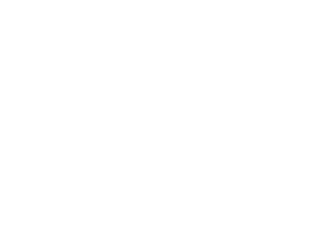
\includegraphics[width=\textwidth]{figures/theory/laminarFlow.pdf}
\caption{This shows the principal difference between laminar and turbulent flow.}
\label{fig:laminar_flow}
\end{figure}


\subsection{Stokes Drag and Stokes's law}
The drag force $F_D$ exerted by a fluid on a spherical particle for $Re << 1$ is found using the so called Stokes's law \cite{introfluid2}

\begin{equation}
F_D = 6\pi \mu R v
\end{equation}

where $v$ is the velocity of the sphere relative to the fluid, $\mu$ is the dynamic viscosity and $R$ is the radius of the sphere. The terminal velocity of the sphere is found by equating the gravitational force $F_G$ acting on the sphere with the drag force. $F_G$ is

\begin{equation}
F_G = \Delta \rho g\cdot \frac{4\pi R^3}{3}
\end{equation}

where $\Delta \rho$ is the difference in density and $g$ is the specific gravity. We find that the terminal velocity of a sinking (or floating) sphere is

\begin{equation}\label{eq:fallingSphere}
v_s = \frac{2}{9} \frac{\Delta \rho}{\mu} g R^2
\end{equation}

%\subsection{Shear}
%
%\subsection{P\'{e}clet Number}
%The p\'{}clet number describes the ratio of thermal noise to other stuff. I really don't know anything about the piclet number.


\section{Jeffrey Orbits}
\label{sec:jeffery}
The Jeffery orbits describe the orientational motion of an ellipsoidal particle in Stokes flow. The general equations of motion for any ellipsoid in shear flow were found by Jeffery\cite{Jeffery} who also solved these equations of motion for axisymmetric ($a_1 \ne a_2 = a_3$) ellipsoidal particles. Solutions for asymmetric particles were found numerically by Yarin \emph{et al.}~\cite{Yarin} who also rewrote the equations in a different but equivalent form. The equations of rotational motion for a triaxial particle in shear flow are in the form of Yarin \emph{et al.}

\begin{subequations}\label{eq:jeffrey}
\begin{align}
\frac{d\theta}{dt} 	&= (g_2 \sin \psi + g_3 \cos \psi ) \sin \theta, \\
\frac{d\phi}{dt} 	&= \tfrac{1}{2} + g_3\sin \psi - g_2 \cos \psi,\\
\frac{d\psi}{dt}	&= g_1 + (g_2\cos \psi - g_3\sin \psi) \cos \theta. \\
\end{align}
\end{subequations}

\noindent The functions  $g_i$ are defined as

\begin{subequations}
\begin{align}
g_1 &= \frac{a_2^2 - a_3^2}{2(a_2^2 + a_3^2)} 
		\left(-\tfrac{1}{2}(\cos^2 \theta + 1 )\sin 2\phi \sin 2\psi + \cos\theta \cos 2\phi \cos 2\psi \right), \\
g_2 &= \frac{a_3^2 - a_1^2}{2(a_1^2 + a_3^2)}
		\left( -\cos\theta \sin 2\phi \sin\psi  +  \cos 2\phi \cos\psi \right), \\
g_3 &= \frac{a_1^2 - a_2^2}{2(a_1^2 + a_2^2)}
		\left( \cos\theta \sin 2\phi \cos\psi + \cos 2\phi \sin\psi \right).
\end{align}
\end{subequations}

\noindent Here $(\phi, \theta, \psi)$ are the Euler angles seen in Figure \ref{fig:eulerangles}. 
%Note that Yarin uses $a_x, a_y, a_z$ in place of $a_1, a_2, a_3$.

Note that the eq. (\ref{eq:jeffrey}) uses the coordinate system from Yarin \emph{et al.}\cite{Yarin} which differ from the one used in this thesis, details are discussed in Johansson \cite{AntonThesis}. Numerical solutions for three different initial conditions for an asymmetric particle are shown in Figure \ref{fig:orbitparams}.

\begin{figure}[H]
\centering
\begin{subfigure}[b]{0.45\textwidth}
\includegraphics[width=\textwidth]{figures/theory/map.pdf}
\caption{A poincare map}\label{fig:orbitmap}
\end{subfigure}\hspace{1em}%
\begin{subfigure}[b]{0.5\textwidth}
\includegraphics[width=\textwidth]{figures/theory/orbit.pdf}
\caption{The time series for the components \\ of the unit vector.}\label{fig:orbitparams}
\end{subfigure}
\caption{A Poincare map and three different orbits for a simulated particle with $\lambda=7$ and $\epsilon=0.05$. The three orbits highlight the three different kinds of motion, the quasi-periodic sign changing orbit in blue, the quasi-periodic sign preserving orbit in red and the periodic orbit in green. We see that while $n_x$ and $n_y$ look qualitatively similar but differ in amplitude for the different orbits, $n_z$ shows three different types of behaviour}
\label{fig:orbittypes}
\end{figure}



Looking at Figure \ref{fig:orbitparams} we see that $n_x$ and $n_y$ are periodic, corresponding to periodic rotation around the $z$-axis. We refer to these rotations as flips. The period $\eta$ of $n_x$ and $n_y$ is for an axisymmetric particle \cite{Jeffery}

\begin{equation}\label{eq:flipRate}
\eta = 2\pi \left( \lambda + \frac{1}{\lambda} \right)\frac{1}{\kappa},
\end{equation}

\noindent where $\kappa$ is the shear rate. 

The time evolution of $\theta$ and $\psi$ for different initial conditions can be plotted in a Poincaré map, also known as a Surface-of-Section (S.O.S.)~\cite{poincare}. This plots the $\psi$ and $\theta$ coordinates each time $\phi = 0$. The successive points on the Poincaré map for each initial condition move and explore certain regions of the surface of section. This region is referred to as the \emph{orbit}. 

For a particle with an asymmetry $\epsilon$ in the range $\left[0.01-0.05\right]$ there are three classes of orbits, depending on the initial condition $\theta_0$.

\begin{enumerate}
\item \textbf{Periodic}: $\left|\theta_0\right| \approx 1$ in which there is little variation and the particle is largely periodic with fluctuations too small to measure.
\item \textbf{Quasi-periodic sign preserving}: For $\left|\theta_0\right|> \theta_b$ the amplitude of $\cos(\theta)$ changes noticeably but does not change sign. Here $\theta_b$ is a breaking point that changes for different $\epsilon$.
\item \textbf{Quasi-periodic sign changing}: For small $\left|\theta_0\right| < \theta_b$ the amplitude of $\cos(\theta)$ changes noticeably and changes sign. 
\end{enumerate}

Simulations of these three different types of orbits for a particle with $\lambda=7$ and $\epsilon=0.05$ are illustrated in Figure \ref{fig:orbittypes}. Figure \ref{fig:orbittypes} shows the orbits on the S.O.S. and Figure \ref{fig:orbitparams} shows the components of $\mathbf{n}$ as a function of time. We can see that while $n_x$ and $n_y$ are periodic, albeit with different amplitudes, the  behaviour of $n_z$ is significantly different for the different orbits. The $n_z \approx 1$  orbit shown in green is constant on the S.O.S and is simply periodic over time. The sign preserving quasi-periodic orbit in red is bent on the S.O.S. We can see in the time series that it is doubly periodic as it peaks with a fixed period but the amplitude of the peaks vary periodically themselves. The sign changing quasi-periodic orbit in blue also peaks periodically with varying peak amplitude but these also change sign, again with a fixed period.


For larger asymmetries $\epsilon > 0.05$ there are chaotic orbits that explore a larger region of the S.O.S. The simulations used do not have long enough time evolutions for the chaotic orbits to fill the regions in the way that quasi-periodic or periodic orbits fill the one dimensional regions that define their orbits. This results in the chaotic orbits appearing as a 'sea' of dots instead of filled lines. Chaotic orbits can been seen around the quasi-periodic sign changing orbits in Figure \ref{fig:orbitmap4}.

\begin{figure}[H]
\centering
\begin{subfigure}[3a]{0.40\textwidth}
\includegraphics[width=\textwidth]{figures/theory/7-1-1.pdf}
\caption{Poincare map for $\lambda = 7, \epsilon = 0$.}\label{fig:orbitmap1}
\end{subfigure}\hspace{1em}%
\begin{subfigure}[3b]{0.40\textwidth}
\includegraphics[width=\textwidth]{figures/theory/7-1o01-1.pdf}
\caption{Poincare map for $\lambda = 7, \epsilon = 0.01$.}\label{fig:orbitmap2}
\end{subfigure} \\
\begin{subfigure}[3a]{0.40\textwidth}
\includegraphics[width=\textwidth]{figures/theory/7-1o05-1.pdf}
\caption{Poincare map for $\lambda = 7, \epsilon = 0.05$.}\label{fig:orbitmap3}
\end{subfigure}\hspace{1em}%
	\begin{subfigure}[3b]{0.40\textwidth}
\includegraphics[width=\textwidth]{figures/theory/7-1o25-1.pdf}
\caption{Poincare map for $\lambda = 7, \epsilon = 0.25$.}\label{fig:orbitmap4}
\end{subfigure} 
\caption{Four Poincare maps for different $\epsilon$. Already at $\epsilon = 0.01$ there are noticeably quasi-periodic 
orbits around the centre at $\cos(\theta) \approx \psi \approx 0$ but it is also a significantly larger region for $\epsilon = 0.05$. For $\epsilon = 0.25$ we can see chaotic orbits surrounding the circular orbits in the centre that appear as a 'sea' of dots.} %q Note that some wavelike pattern can appear to exist in the figure \ref{fig:orbitmap2} and  \ref{fig:orbitmap2}, this is caused by aliasing/compression issues with printing several curved lines close together.}\label{fig:orbitmaps}
\end{figure}

\subsection{Winding number} \label{sec:winding}
The quasi-periodic orbits are also referred to as doubly-periodic~\cite{Yarin}. It is called doubly-periodic to emphasize the fact that the amplitude of the short period $\theta_2$ also varies periodically with period $\theta_1$. The ratio between the two periods is referred to as the winding number $\omega$ referring to the winding around a unit torus. The shorter period $\theta_2$ corresponds to rotations around the small cross section and the longer period $\theta_1$ corresponds to rotations around the large circumference of the torus. The winding number is defined as \cite{introchaos}

\begin{equation}
\omega_{def}  = \lim\limits_{n \rightarrow \infty} \frac{f^n(\xi) - \xi_0}{n}.
\end{equation}

where $\xi$ is the angle around the large circumference of the torus and $f^n(\xi)$ is the shift caused in $n$ rotations around the smaller axis. 
Applying this to our double-periodic orbits $\xi$ would be the angle with period $\theta_1$ and $n$ the number of flips with period $\theta_2$. 
Since we cannot measure $\xi$ I consider it more comprehensible to consider the inverse winding number: The number of flips necessary to 
complete one period of $\xi$. This can be measured as is shown in Figure \ref{fig:windingDef}. If we measure over several $\theta_1$ peaks the average winding number approximates the real one. We refer to the this inverse winding number as $\omega$ and it is given by

\begin{equation}\label{eq:winding}
\omega = \frac{\theta_1}{\theta_2}.
\end{equation}

\noindent The winding number of the quasi-periodic sign preserving orbit from Figure \ref{fig:orbittypes} and the way we approximate $\theta_1$ (and thereby $\omega$) is illustrated in Figure \ref{fig:windingDef}.

\begin{figure}[H]
\begin{center}
\includegraphics[width=0.7\textwidth]{figures/theory/WindingNrFixed2.pdf}
\end{center}
\caption{The quasi-periodic sign preserving orbit from Figure \ref{fig:orbitparams} over a longer time, highlighting the short period $\theta_2$ which is simply the period of $\phi$ and the longer period $\theta_1$. We find the inverse winding number as the ratio between the longer and shorter periods.}
\label{fig:windingDef}
\end{figure}

%This can also be thought of as the number of intersections on the surface of section before coming back to the initial condition, divided by the number of laps. A lap for a circular orbit is a rotation around the center whereas for a flat orbit it is moving along length of the orbit. asdasd, see figure MAKE A FIGURE. 
The winding number is the same for any point along a quasi-periodic orbit on a Poincaré map but it is different for different orbits as well as for different asymmetries. The winding numbers for orbits along $\psi=0$ for $\epsilon=\{0.01, 0.05, 0.10\}$ can be seen in Figure \ref{fig:windingdifferent}. The difference in winding number between the different $\epsilon$ for the sign changing orbits are almost a factor 2. This means that if we can measure the winding number for a sign changing orbit it allows us to approximate the asymmetry of the particle even though the variation in $n_z$ are identical. Without looking at the winding number we cannot determine if a particle with an orbit close to $n_z = 0$ and small variations in amplitude is close to symmetric or not.
 
\begin{figure}[H]
\begin{center}
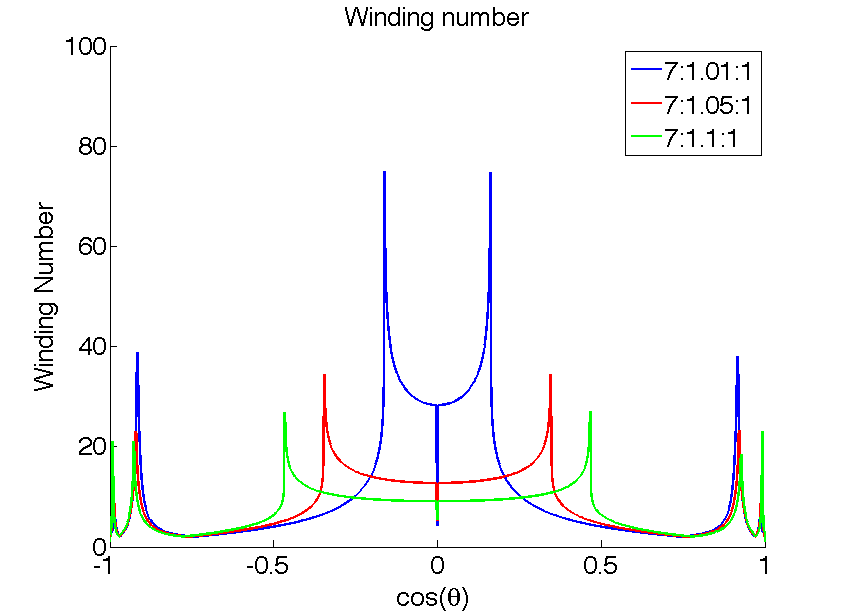
\includegraphics[width=0.7\textwidth]{figures/theory/WindingTrend.png}
\end{center}
\caption{The winding number for $\psi_0 = 0$ and $\lambda = 7$ as a function of $\cos(\theta_0)$ for three different asymmetries, $\epsilon = 0.01$, $\epsilon = 0.05$ and $\epsilon = 0.10$. The sharp edge that occurs at different points for the different asymmetries, but centred around zero, is where the sign changing orbits end and sign preserving orbits begin, denoted by $\theta_b$. We see that a lower asymmetry leads to a sharper difference between the sign changing and the sign preserving orbits and that higher asymmetry in general leads to lower winding numbers on average.}
\label{fig:windingdifferent}
\end{figure}

% Not quite sure how far in depth I should go here
\section{Kalman filter}
% Should I even have this section?

\chapter{Method}

\section{Experimental Setup}
\label{sec:exp_setup}
The orientational motion of $\mu$m sized particles suspended in a liquid was investigated by pumping the liquid through a microfluidic channel using a syringe pump. The channel is placed on a moveable stage on top of a microscope. A particle is tracked by moving the stage to match the center of mass velocity of the particle in the channel and thus keep the particle stationary in the field of view of the microscope. Connected to the microscope is a CCD camera recording the images and these movies are saved on a computer. 

When the tracked particle gets within \unit[1]{cm} of the inlets on the channel the flow is reversed. In order to reduce sudden impact of the pressure difference the reversals are incremental. At the start of a reversal the infusion/withdrawal rate is reduced by 50\% for 10 seconds, then stopped completely for 10 seconds. After this the flow is reverted at 50\% of the normal flow rate for another 10 seconds before resuming at full speed. 

We refer to the data of a particle along one length of the channel a \textbf{stretch} and a series of stretches for a single particle a \textbf{measurement}. A sketch of the experimental setup can be seen in figure \ref{fig:setupsketch}, and a photograph of the actual setup in figure \ref{fig:setuppicture}. 

Between measurements, optical tweezers constructed by A. Laas were used to change the orientation of the particle. For details on optical tweezers function see the introductory guide from Stanford \cite{OpticalTweezer} or Laas thesis \cite{alexanderThesis}. 


\begin{figure}[H]
\centering
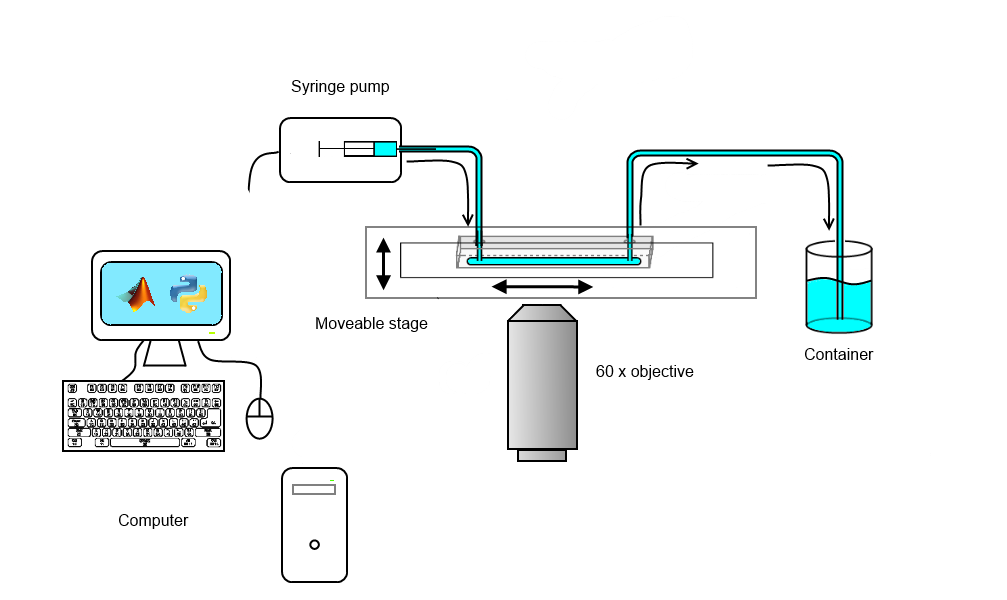
\includegraphics[width=0.8\textwidth]{figures/method/setupsketch.png}
\caption{Sketch of the set up. The computer controlled stage moves over the microscope. The pump reverses when the tracked particle gets close to the inlets of the channel.}\label{fig:setupsketch}
\end{figure}

% Have both this zoomed out and the zoomed in view I think
\begin{figure}[H]
\centering
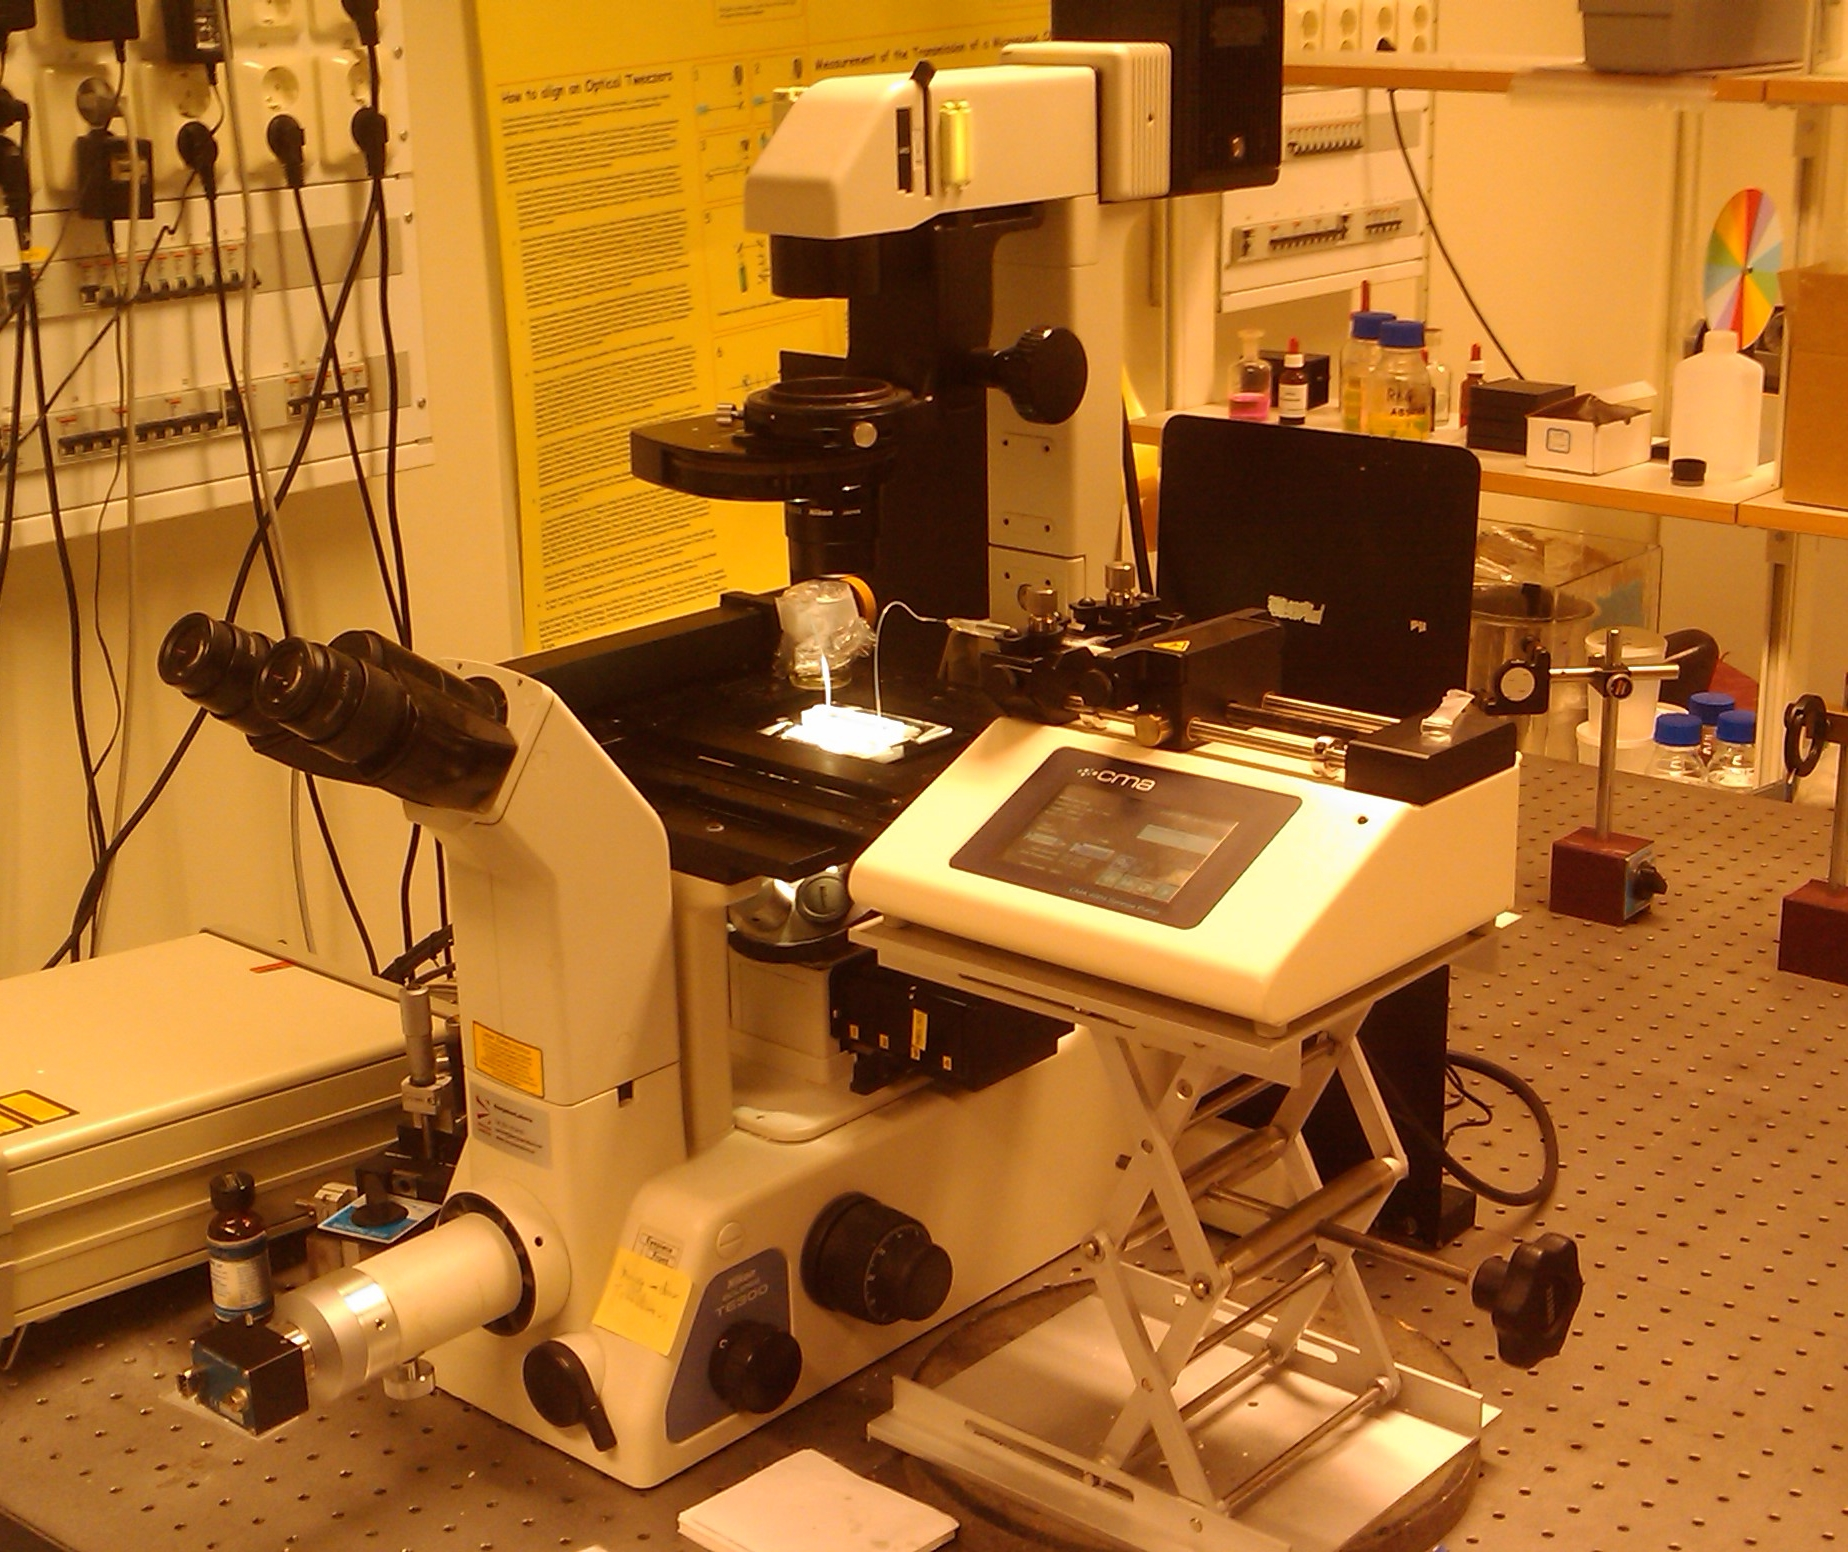
\includegraphics[width=0.8\textwidth]{figures/method/ExperimentalOverview.jpg}
\caption{Overview of the set up. The microscope to the left and the syringe pump to the right. In the center is the channel and the outlet container is seen behind it. The CCD camera is mounted on the left side of the microscope and cannot be seen in this picture.}\label{fig:setuppicture}
\end{figure}


The microfluidic channel is \unit[40]{mm} long, \unit[2.5]{mm} wide and approximately \unit[150]{$\mu$m} deep. The channel is made from Polydimethylsiloxane (PDMS) and plasma bonded to a microscope slide. A more detailed description of the process can be found from the Center for Computer Integrated Systems for Microscopy and Manipulation~\cite{PDMS}. This material and procedure is chosen so that a channel that gets filled with dirt or breaks can cheaply and easily be replaced. PDMS is also non-reactive and highly transparent. A sketch of the channel can be seen in figure \ref{fig:channelsketch}, and a photograph of an actual channel in figure \ref{fig:channelpicture}. 

\begin{figure}[H]
\centering
\begin{subfigure}[b]{0.45\textwidth}
\includegraphics[width=0.9\textwidth]{figures/method/channelDetail.pdf}
\caption{Sketch of the channel}\label{fig:channelsketch}
\end{subfigure}
\begin{subfigure}[b]{0.45\textwidth}
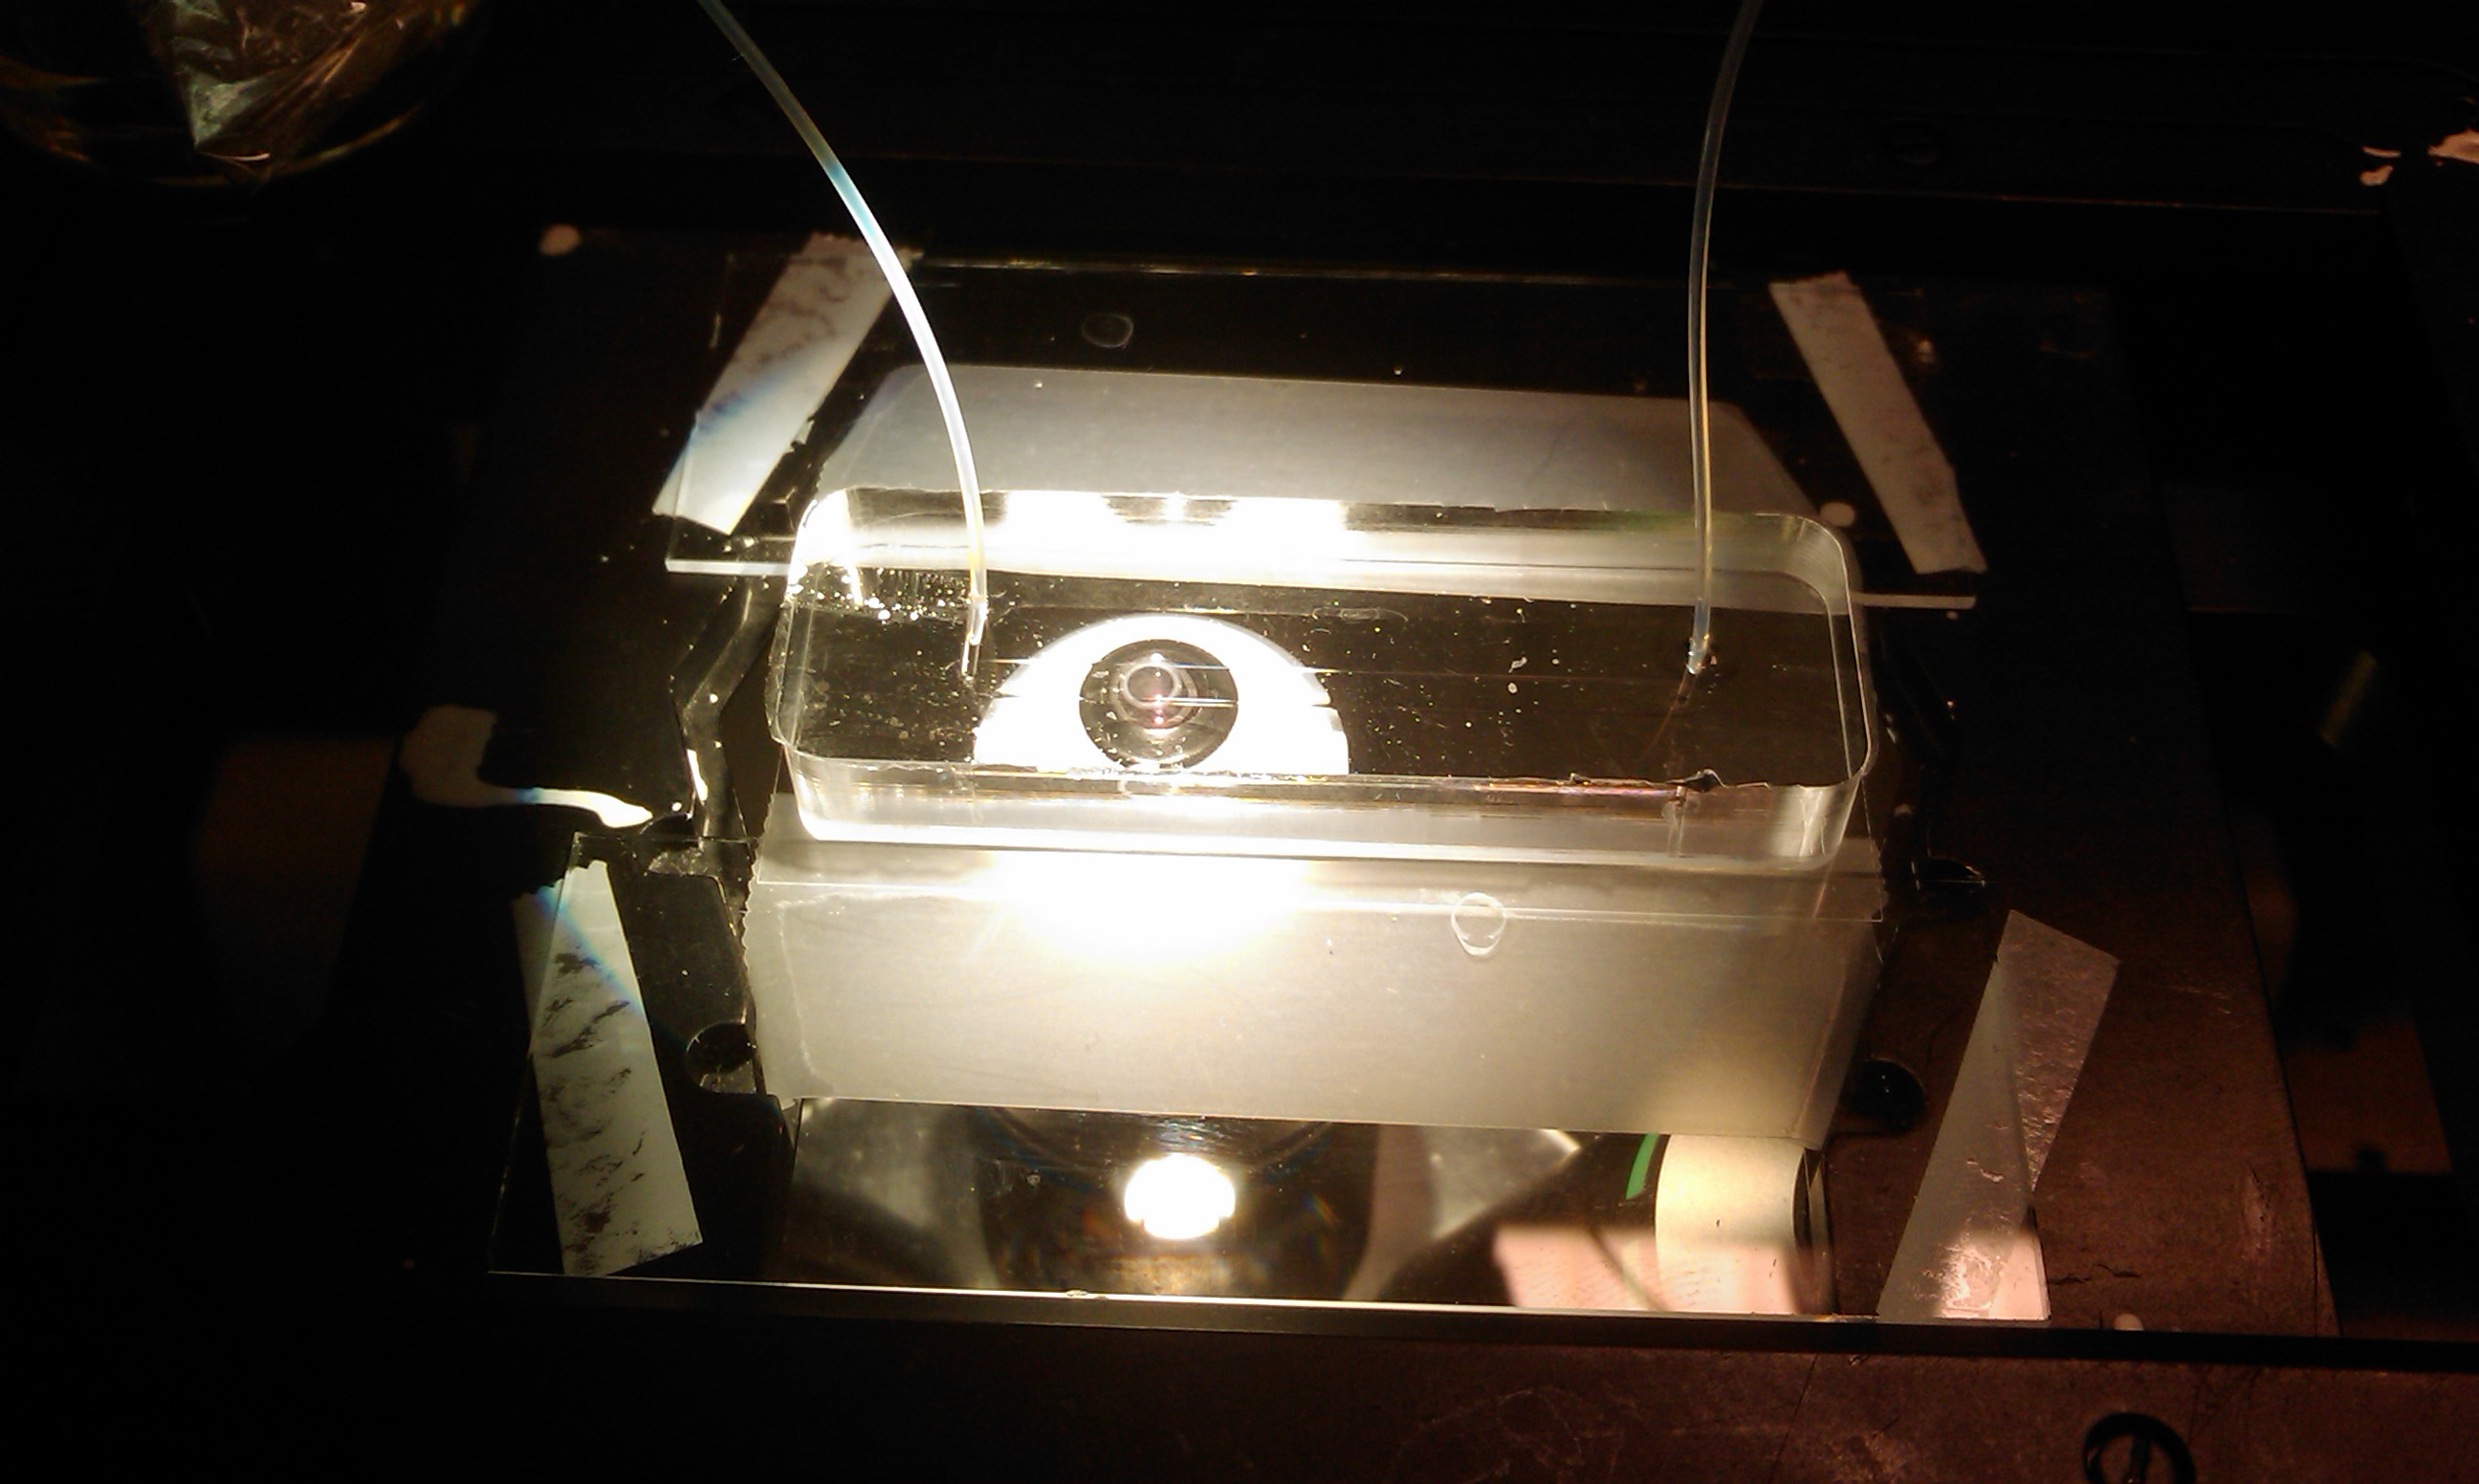
\includegraphics[width=0.9\textwidth]{figures/method/ChannelZoomed.jpg}
\caption{Picture of the channel}\label{fig:channelpicture}
\end{subfigure}
\caption{A sketch of the channel as well as a picture of the channel as it is set up during a measurement. The channel is only \unit[150]{$\mu$m} deep, but the PDMS surrounding it is around 15 mm to try and prevent the channel from expanding and contracting too much.}
\label{fig:channel}
\end{figure}

% rewrite
In order to find the maximum flow speed of the channel we need to know the flow profile. Using the software employed by Johansson \cite{AntonThesis} we obtain the flow profile that can be seen in figure \ref{fig:flowprofile}. Integrating 
the flow profile over the entire surface will give us an effective flow area, essentially how large the channel 'actually' is. 
Using the flow profile from figure \ref{fig:flowprofile} we find that the effective flow area is $\unit[0.14]{mm^2}$. With a pump rate of \unit[7.5]{$\mu$l/minute} we get a maximum velocity of \unit[0.90]{mm/s} for the liquid.

% PIcture of the channel meassurements here 


% Picture of channel flow profile
\begin{figure}[H]
\begin{center}
\includegraphics[width=0.7\textwidth]{figures/method/flowprofile.pdf}
\end{center}
\caption{The theoretical estimation of the flow profile. Image generated with software from Johansson \cite{AntonThesis}, used with permission.}
\label{fig:flowprofile}
\end{figure}

\noindent We need to confirm that the flow is has no inertial effects. We can calculate the maximum Reynolds number using eq \ref{eq:reynolds}, the \unit[3]{$\mu$m} length rods, and our maximum flow speed.

\begin{equation}
\operatorname{Re_p} = \frac{U L \rho}{\mu} 
\leq \frac{9.0\cdot 10^{-4} \cdot 3 \cdot 10^{-3} 2.5 }{24 \cdot 10^{-3}} 
\approx	 	2.78  \cdot 10^{-6} \ll 1
\end{equation}

This should satisfy the conditions of validity for the Jeffrey equations. 

To track the particles the channel is put in a moveable stage on a confocal microscope. The entire setup can be seen in figure \ref{fig:setuppicture}



\subsection{List of equipment}
 The equipment used during the experiment is as follows
\begin{itemize}
\item Leica DFC350 FX digital camera 
\item Nikon Eclipse TE 300 microscope
\item Nikon 60x water immersion objective
\item Märzhäuser Wetzlar 'LStep-eco' step engine
\item CMA 4004 syringe pump
\item Ytterbium fiber laser  % What laser?
\end{itemize}

%
%\subsection{Density matching}
%\begin{equation}
%\rho_{a} = 	\frac {m_{a}}{V_{a}} =
%				\frac{V_{b}\rho_{b} + V_{mix}\rho_{mix}}{V_b + V_{mix}} 
%\end{equation}
%So if we want to find $V_{mix}$ we get
%\begin{equation}
%V_{mix} = \frac{ V_{b}(\rho_{b} - \rho_{a})}{\rho_{a} - \rho_{mix}} 
%\end{equation}
%
	


% This should not be a chapter but a section of the experimental setup. Maybe a section of 
% that should be improvements and I can include the Automated tracking can be part of that
% I should also ask Dag if it's reasonable to include a section of attempted improvements, as
% a guideline to anyone who tris to replicate the experiment both about what can be done (for inspiration)
% but then as a caution that while you may try this it did not work for us

TODO:
READ UP ON THE EFFICIENCY OF THE CANNY EDGE DETECTION
TAKE AN IMAGE OF THE STATIC NOISE REDUCTION (DOES IT ACTUALLY WORK?!)
GET AN IMAGE OF BEFORE AND AFTER SMOOTHING, PREFERABLY INCLUDE A CANNY EDGE DETECTION OF BOTH 
WRITE ABOUT THE TIME IT TAKES TO DO VARIOUS STUFFS (IS THIS NEEDED?)
GET MORE SOURCES IN THE THEORY SECTION
IN PARTICULAR:
Looking up reynolds number sources, "creeping motion" might be a relevant term
Add our measured visc and add it to citations, maybe add Dag how to cite that?


JEFFREY ORBIT STUFF:
Make a picture illustrating the various angles
Have a picture of some jeffrey orbits

EXPERIMENTAL SETUP STUFF:
Include the distribution of lengths, either meassured or from nippon


\section{Particle tracking}


\subsection{Noise Reduction}
The first step in tracking a particle is to correctly identify it in the image given. To do this we want to eliminate as much noise from the image as we can. The first type of noise we will eliminate is static noise, this is noise present in every image and results from dirt or scratches on the lens of the camera or microscope. 
The easiest solution to such noise would of course be to clean the instruments, but despite numerous attempts of carefully cleaning every surface a noticeable of static noise would always remain. 

This means one must use algorithmic noise reduction methods to remove this noise. The method employed is a simple averaging that takes N pictures at different positions in the channel to generate an average image where any particular features of the channel would disappear and only the static noise remain. This can be seen in figure STATIC NOISE REDUCTION IMAGE,


\subsection{Canny Edge Detection}
The Canny Edge invented by John Canny in his 2011 paper the canny of cane detection is generally considered the most advanced and best performing edge detection of the simple filter functions. 
Without going in to the finer details, given an image matrix $\mathbf{I}$ where each value corresponds to the light intensity $i_{x,y}$of that pixel at index $x,y$ the Canny edge detector will try to find the cohesive pixels $E = \{e_1, e_2... e_n\}$ where there is a noticeable change in intensity. In other words, what we call an "edge" an image. 

This is accomplished in two steps. First a Sobel Filter edge image is computed by looking at the change in intensity at every pixel from 3 possible directions and averaging these. 

S = MATHEMATICS OF SOBEL

We then consider a Then, a pixel 

$p_{x,y} \in E \text{if} S(x,y) > T_{high}$

where $T_{high}$ is a predetermined threshold value. 

Secondly we recursively check all pixels neighbouring an edge

MATH?

 if they are higher than some threshold value $T_low$. if they are, they are also considered part of the edge. This is repeated until no more pixels are added. An image illustrating this process can be seen in figure FIG. The benefit of the Canny edge detection over the simpler Sobel is that it is much easier to detect cohesive objects that vary in intensity without getting a lot of other noise in the image. The only real drawback of the Canny Edge detection is the computation time, and thus the implementation from the Open Computer Vision (OCV) was used, as this is a heavily optimized routine written in C++ with real time uses in mind. Thanks to this the computing for the Canny Edge of a 260x260 Image takes about X ms and thus is of little importance in the overall time per frame.

After noise reduction the Canny Edge Detection is used to find the most significant edges in the image. 

\subsection{Contour detection and selection}

Once an edge image has been generated, the OCV package has another useful function, \texttt{Contours} which returns a list of every contiguous group of edge pixels. If we have chosen the threshold values to the edge detection correctly, this should include the particle or a good approximation of it. 

In order to find the correct contour, a few techniques are used to find the correct contour.

First particles whose total size is less than some minimum value, $ n_{min}$ or larger than some maximum value $n_{max}$ are ignored. Then the position $pP_i$ of each contour $C_i={p_1,p_2...p_n}$ is calculated as the average pixel position

\[
P_i = \sum_{j}^n p_j/n
\]
This position is compared to the expected position of the Kalman filter, which the very first frame is the middle position. 

Finally a 'thinness value' is calculated according to eq \ref{eq:thinness}

\begin{equation}\label{eq:thinness}
w_{thin}\left(\frac{ n}{d_{max}^2}\right)^2
\end{equation}. 
where $w_{thin}$ is a weighting constant, $n$ is the number of pixels in the contour and $d_{max}$ is the longest distance between two pixels in the 
where I am not really sure I should do this now that I have so few particles, but I do it none the less!

\subsection{Stabilizing the tracking}
Once a state estimation has been made, we want to adjust the speed of the step engine to, as best as possible, match that of the particle. This is done by looking both the position and velocity of the particle and going through the conditional statements shown in figure CONDITIONAL CORRECTION VECTOR. 

The goal is to limit the amount of corrections made, as changing the velocity is rather time intensive as discussed in section \ref{sec:time considerations}, as well as keeping the particle stable. There is also no point in trying to completely eliminate movement
% % About how to choose the correction vector and communicate with the step engine

\subsection{Time Considerations}\label{sec:time considerations}
A higher FPS will allow the particle detection to be better, improve the position saving and allow the particle tracking to be more stable as well. So maximizing the FPS, ie reducing the computational time of each task, is a clear goal for a good automated tracking. A list of the different tasks and their average execution times can be seen in table \ref{tab:benchmarks}

\begin{table}[H]
 \begin{tabular}{l | c | c } 
 Task  			&  Average time & Std deviation \\
 Capture screen & 1000 			& 200 \\
 Find edges 	& 200			& 20 \\
 \end{tabular}
 \caption{}
 \label{tab:benchmarks}
\end{table}

We can clearly see that FPS is limited primarily by three routines: The screen capture routine, the change velocity routine and finally the save position routine. The first and last are unavoidable and must be done every frame by definition if we are interested in knowing the particles position as well as possible. This means we simply want to use the velocity correction as little as possible. Since the time constraint is in the communication with the step engine, there is not any optimization to be done here, at least not within the scope is this thesis. 


\section{Kalman Filter}
	When the particle is at constant motion in the channel the equations of motion give us
	\begin{equation}
	\left[
	\begin{array}{c}
	  x_n	 \\
	 	  v_{x,n} \\ 
	  y_n	 \\
	  v_{y,n} 
	\end{array} 
	\right]
	 =
	 \begin{bmatrix}
	  x_{n-1} & + v_{x,n-1} \\
	  v_{x,n-1}       & ...		 \\
	  y_{n-1} &+v_{y,n-1}  \\
	  v_{y,n-1}       &		\\
	 \end{bmatrix}
	+
	\left[
	\begin{array}{c}
	0 \\
	c_{xn} \\
	0 \\
	c_{yn}
	\end{array}
	\right]
	%	x_n \right] = \left[ x_{n-1}+ v_{n+1} \right]\\
	%	v_{xn}
		y_n
		v_{yn}
	\end{equation}
	
	We can rewrite this in matrix form as
	
	\begin{equation}
	\left[
	 \begin{array}{c}
	 x_{n} \\
	 v_{x,n}\\
	 y_{n}\\
	 v_{y,n}
	 \end{array}
	 \right]
	 =
	 \begin{bmatrix}
	  1 & 	\Delta t & 	0 & 	0 \\
	  0 & 	1 & 	0 & 		0 \\
	  0 & 	0 & 	1 & \Delta t  \\
	  0 & 	0 & 	0 & 		1 \\
	 \end{bmatrix}
	 \cdot
	 \left[
	 \begin{array}{c}
	 x_{n-1} \\
	 v_{x,n-1}\\
	 y_{n-1}\\
	 v_{y,n-1}
	 \end{array}
	\right]
	 +
	 \begin{bmatrix}
	   0 & 	0 & 	0 & 	0 \\
	   0 & 	1 &		0 & 	0 \\
	   0 & 	0 & 	0 &    	0 \\
	   0 & 	0 & 	0 & 	1 \\
	  \end{bmatrix}
	  \cdot
	  \begin{array}{c}
	  0 \\
	  c_{x,n-1} \\
	  0 \\
	  c_{y,n-1}
	  \end{array}
	\end{equation}
	
	Now if we want to transform this to the measured data we have to simply multiply by a constant pixel-to-meter constant, which has been meassured to be around $1/940=1.06\cdot 10^{-3}$
	
	\begin{equation}
	Q = 
	 \begin{bmatrix}
	  0 & 	0 & 	0 & 	0 \\
	   0 & 	1 &		0 & 	0 \\
	   0 & 	0 & 	0 &    	0 \\
	   0 & 	0 & 	0 & 	1 \\
	  \end{bmatrix}
	\end{equation}
	
	Which we can easily re-write as a Kalman filter 
	\begin{equation}
	\hat{\mathbf{x}}_{n} = \mathbf{A}_n\mathbf{x_{n-1}} + \mathbf{B}_n \mathbf{u}_n + \mathbf{w}_n
	\end{equation}
	\begin{equation}
	\hat{\mathbf{P}}_n = \mathbf{F}_n \mathbf{P}_{n-1} \mathbf{F}^{T}_{n} + \mathbf{Q}_n
	\end{equation}
	with 
	\begin{eqnarray}
	\mathbf{x}_n &= 
	\left[
	x_n 
	v_{x,n} 
	y_n 
	v_{y,n}
	\right]^T \\
	\mathbf{A} &= 
	\begin{bmatrix}
	  1 & 	\Delta t & 	0 & 	0 \\
	  0 & 	1 & 	0 & 		0 \\
	  0 & 	0 & 	1 & \Delta t  \\
	  0 & 	0 & 	0 & 		1 \\
	\end{bmatrix} \\
	\mathbf{B}_n &= 
	 \begin{bmatrix}
	   0 & 	0 & 	0 & 	0 \\
	   0 & 	1 &		0 & 	0 \\
	   0 & 	0 & 	0 &    	0 \\
	   0 & 	0 & 	0 & 	1 \\
	  \end{bmatrix}
	\\
	\mathbf{u}_n &=
	\left[
	  \begin{array}{c}
	  0 \\
	  c_{x,n-1} \\
	  0 \\
	  c_{y,n-1}
	  \end{array}
	  \right] 
	\end{eqnarray}
	
	and we add the update part as
	\begin{eqnarray}
	&\mathbf{K}_n = \hat{\mathbf{P}}_n \mathbf{H}^T_n(\mathbf{H}_n \hat{\mathbf{P}}_n \mathbf{H}^T_n	) \\
	&\mathbf{x_n} = \hat{\mathbf{x}}_n + \mathbf{K}_n(\mathbf{y} - \mathbf{H}_n\hat{\mathbf{x}}_n) \\
	&\mathbf{P}   = (\mathbf{I} - \mathbf{K}_n\mathbf{H}_n)\hat{\mathbf{P}}_n
	\end{eqnarray}
	
	
	
	
	


\chapter{Results}
The aim of these measurements is to show that the particles follow the Jeffery orbits and to show that they exhibit quasi-periodic or periodic motion for different initial conditions. In order to show that there are no significant disturbance we examine the reversal. If it reverts perfectly there has been no noise or inertial effects.

During the work of this thesis a large number of movies of particles have been recorded with gradual improvements to the setup primarily in terms of density matching, particle density (the number of particles per liquid volume)and  bubble elimination. In this section we present the data from two different particles. These were the only particles where there were good reversals for several stretches for both quasi periodic and periodic orbits. One referred to as particle A, the other as particle B. Particle A is approximately \unit[24]{$\mu m$} long so it has an aspection ratio $\lambda \approx 8$, particle B is approximately \unit[20.5]{$\mu m$} long so it has an aspection ratio $\lambda \approx 7$. The measurements in this section were done together with Alexander Laas.

We started each measurement at an approximate depth $D$ and at position $p_0 = (x_0, z_0)$ in the channel relative to the inlet on the right, closer to the pump. We have assumed that the shear is entirely in the $y$ direction when doing 	our theoretical analysis. This means the flow profile has to be almost entirely flat in the $z$-direction which it only is if the particle is close to the centre. Variations do occur but when are less than \unit[10]{$\mu$m} as is seen in figure \ref{fig:particleAsink}.

\newpage
% LOLOLOLOLOLOL
\chapter{Discussion}

% % STUFF I SHOULD CITE % %
%http://ncds.technion.ac.il/userfiles/publications/jfm97ygr_ellipsoid.pdf
\appendix
\chapter{Raw data}

%\section{$\mathbf{\lambda}$ of about 6}
%These are the particles with a $\lambda = 6 \pm 0.5$
%\subsection{Particle 1}

\begin{figure}[H]
\centering
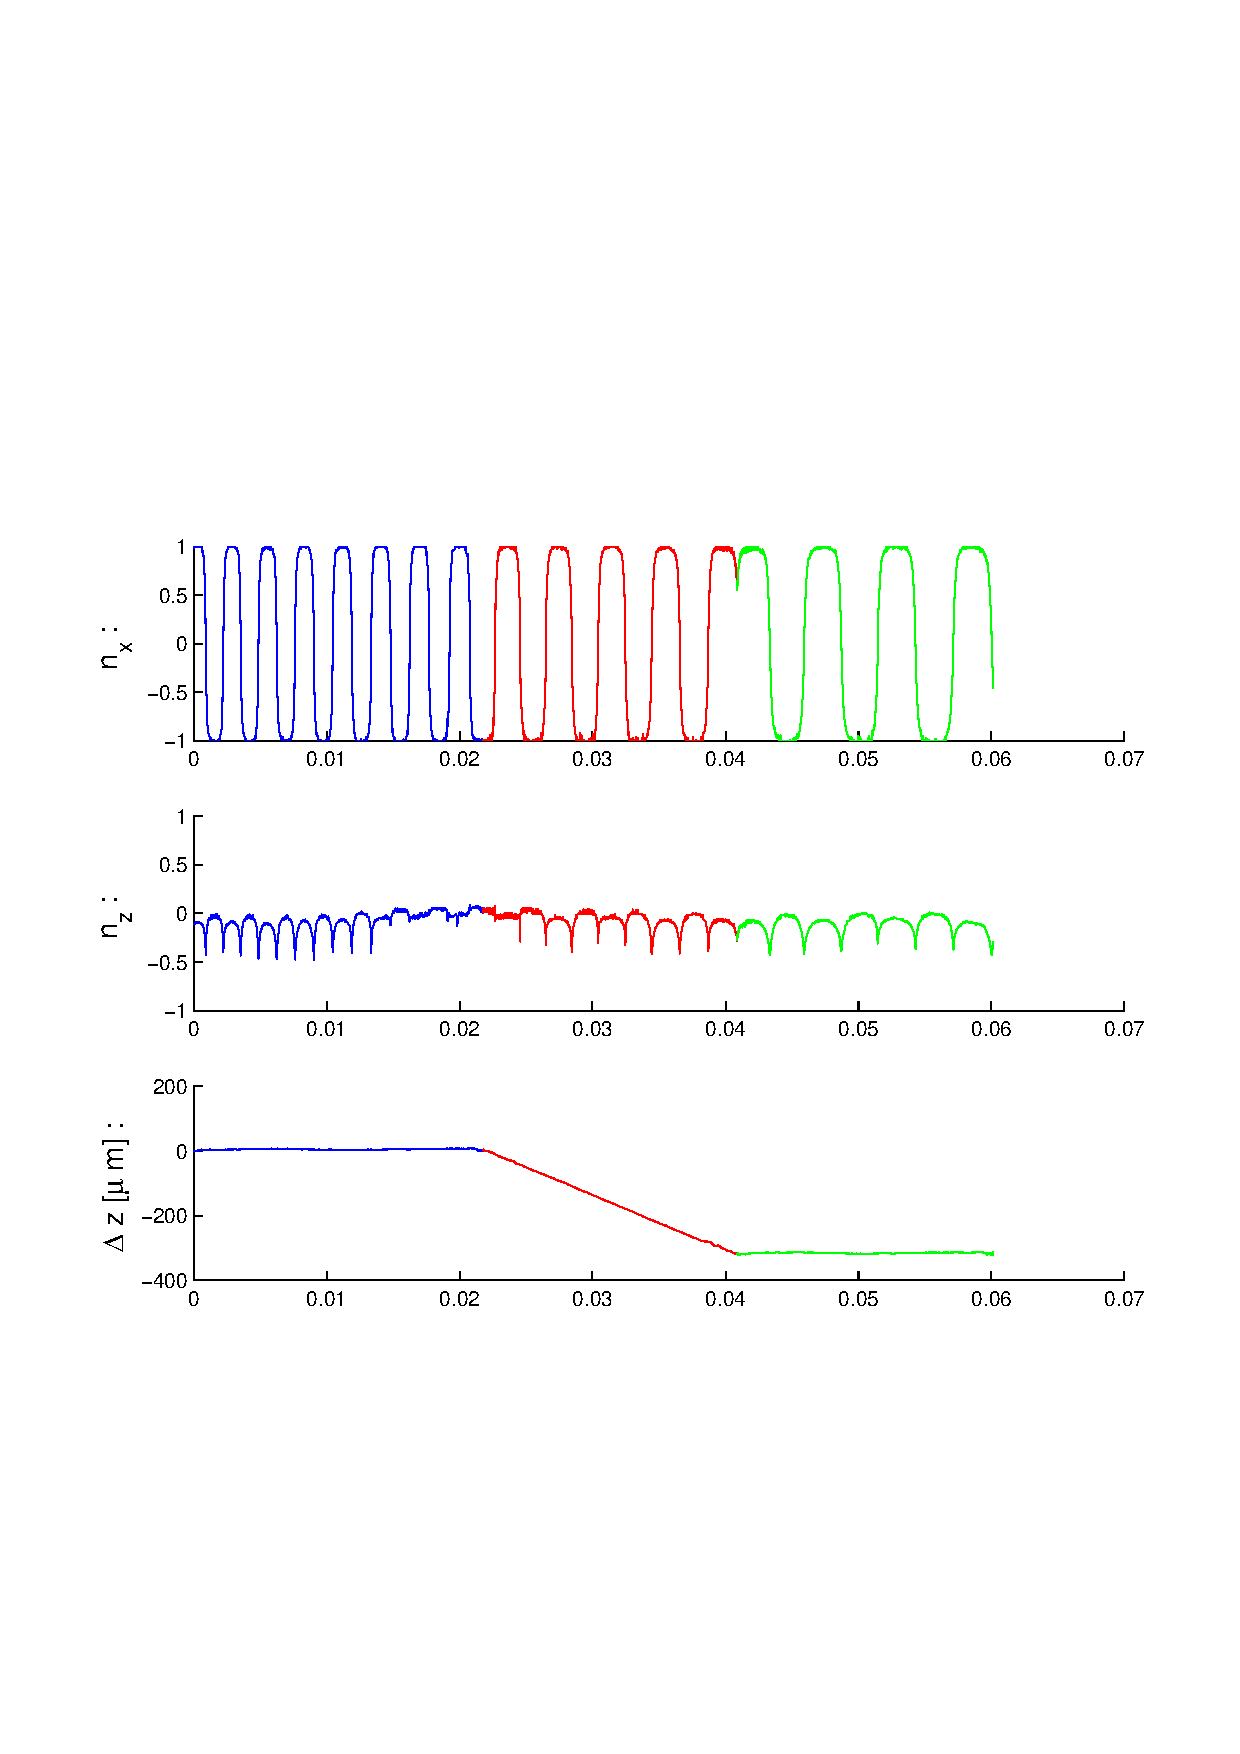
\includegraphics[width=0.8\textwidth]{Images/Particle 1/Particle1.pdf}
\caption{Particle 1: $ \lambda: 6.1591$Depth: 160 out of $200 \mu $ m}
\end{figure}

\begin{figure}[H]

\centering

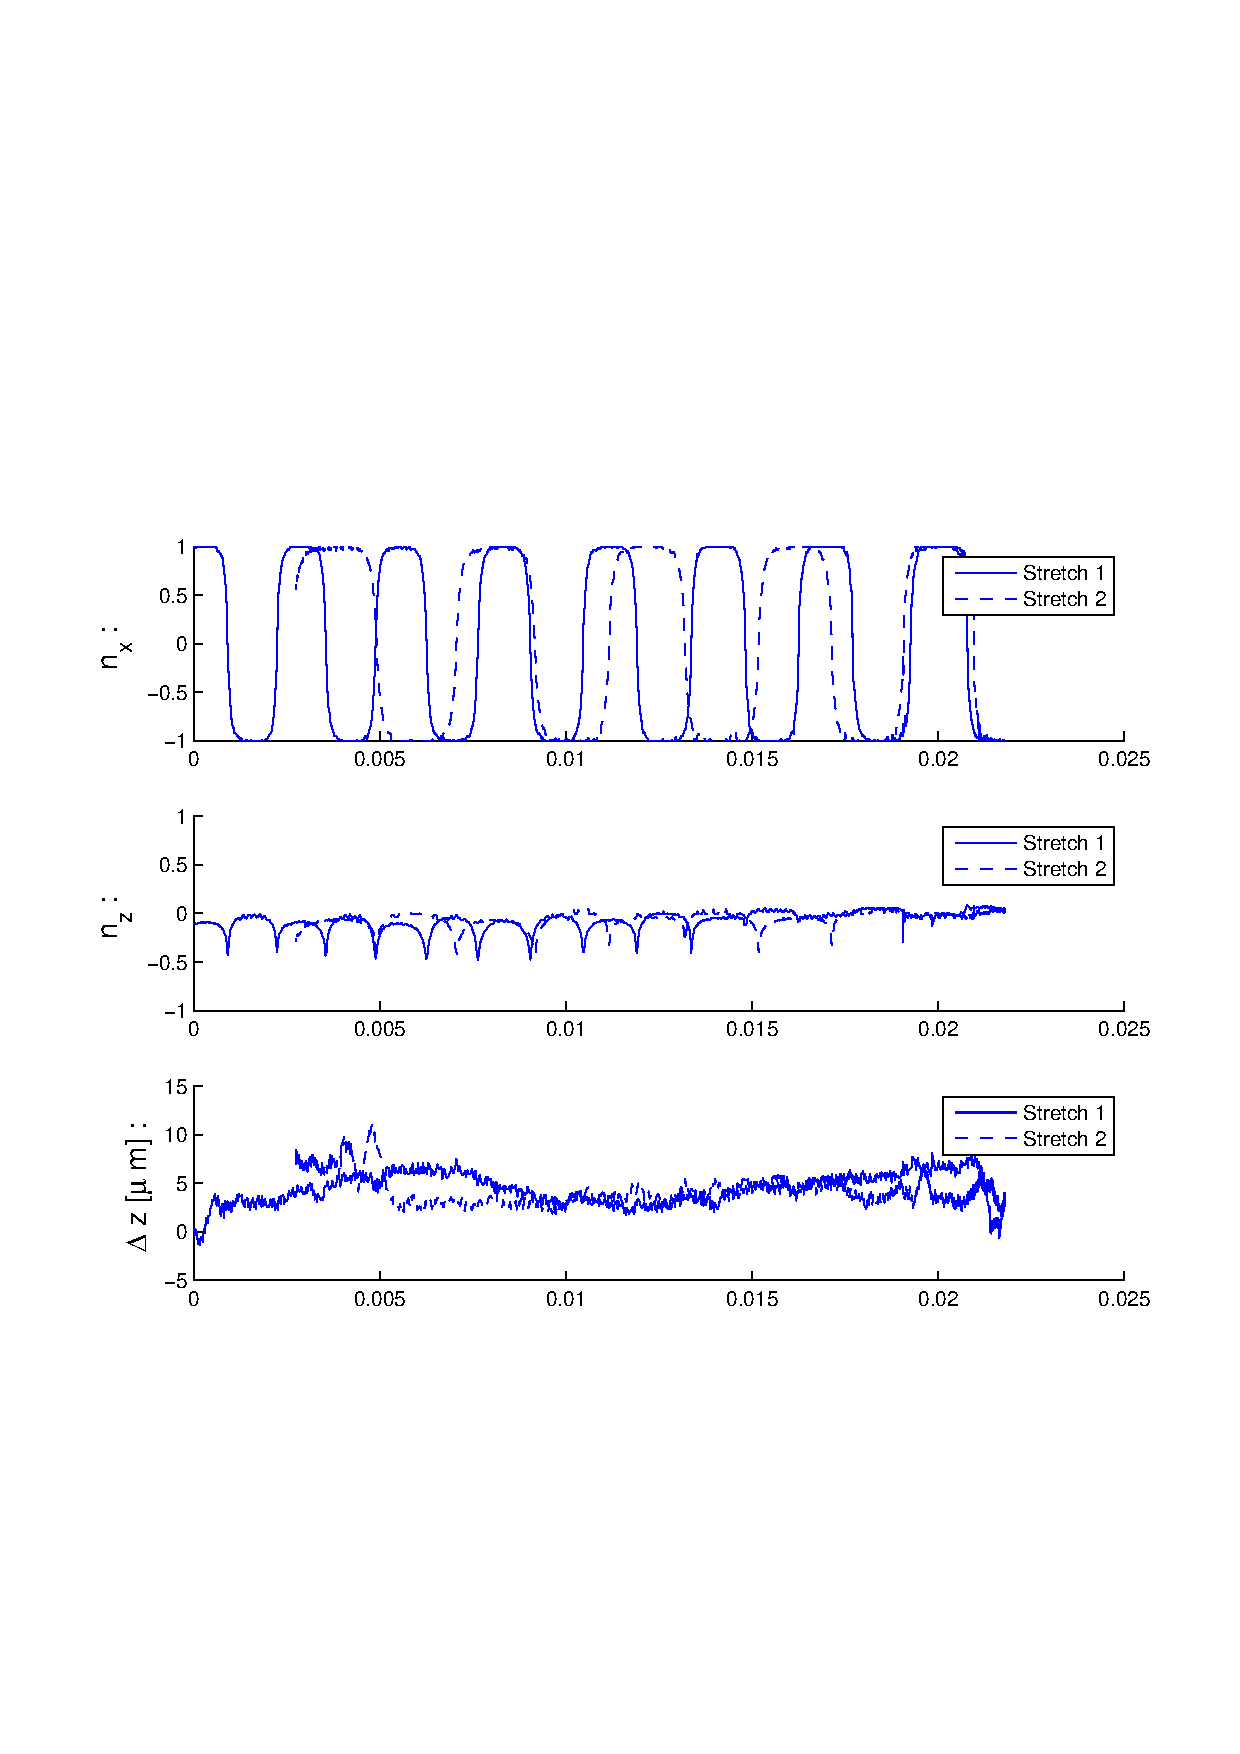
\includegraphics[width=0.8\textwidth]{Images/Particle 1/Stretch1.pdf}

\end{figure}

\begin{figure}[H]

\centering

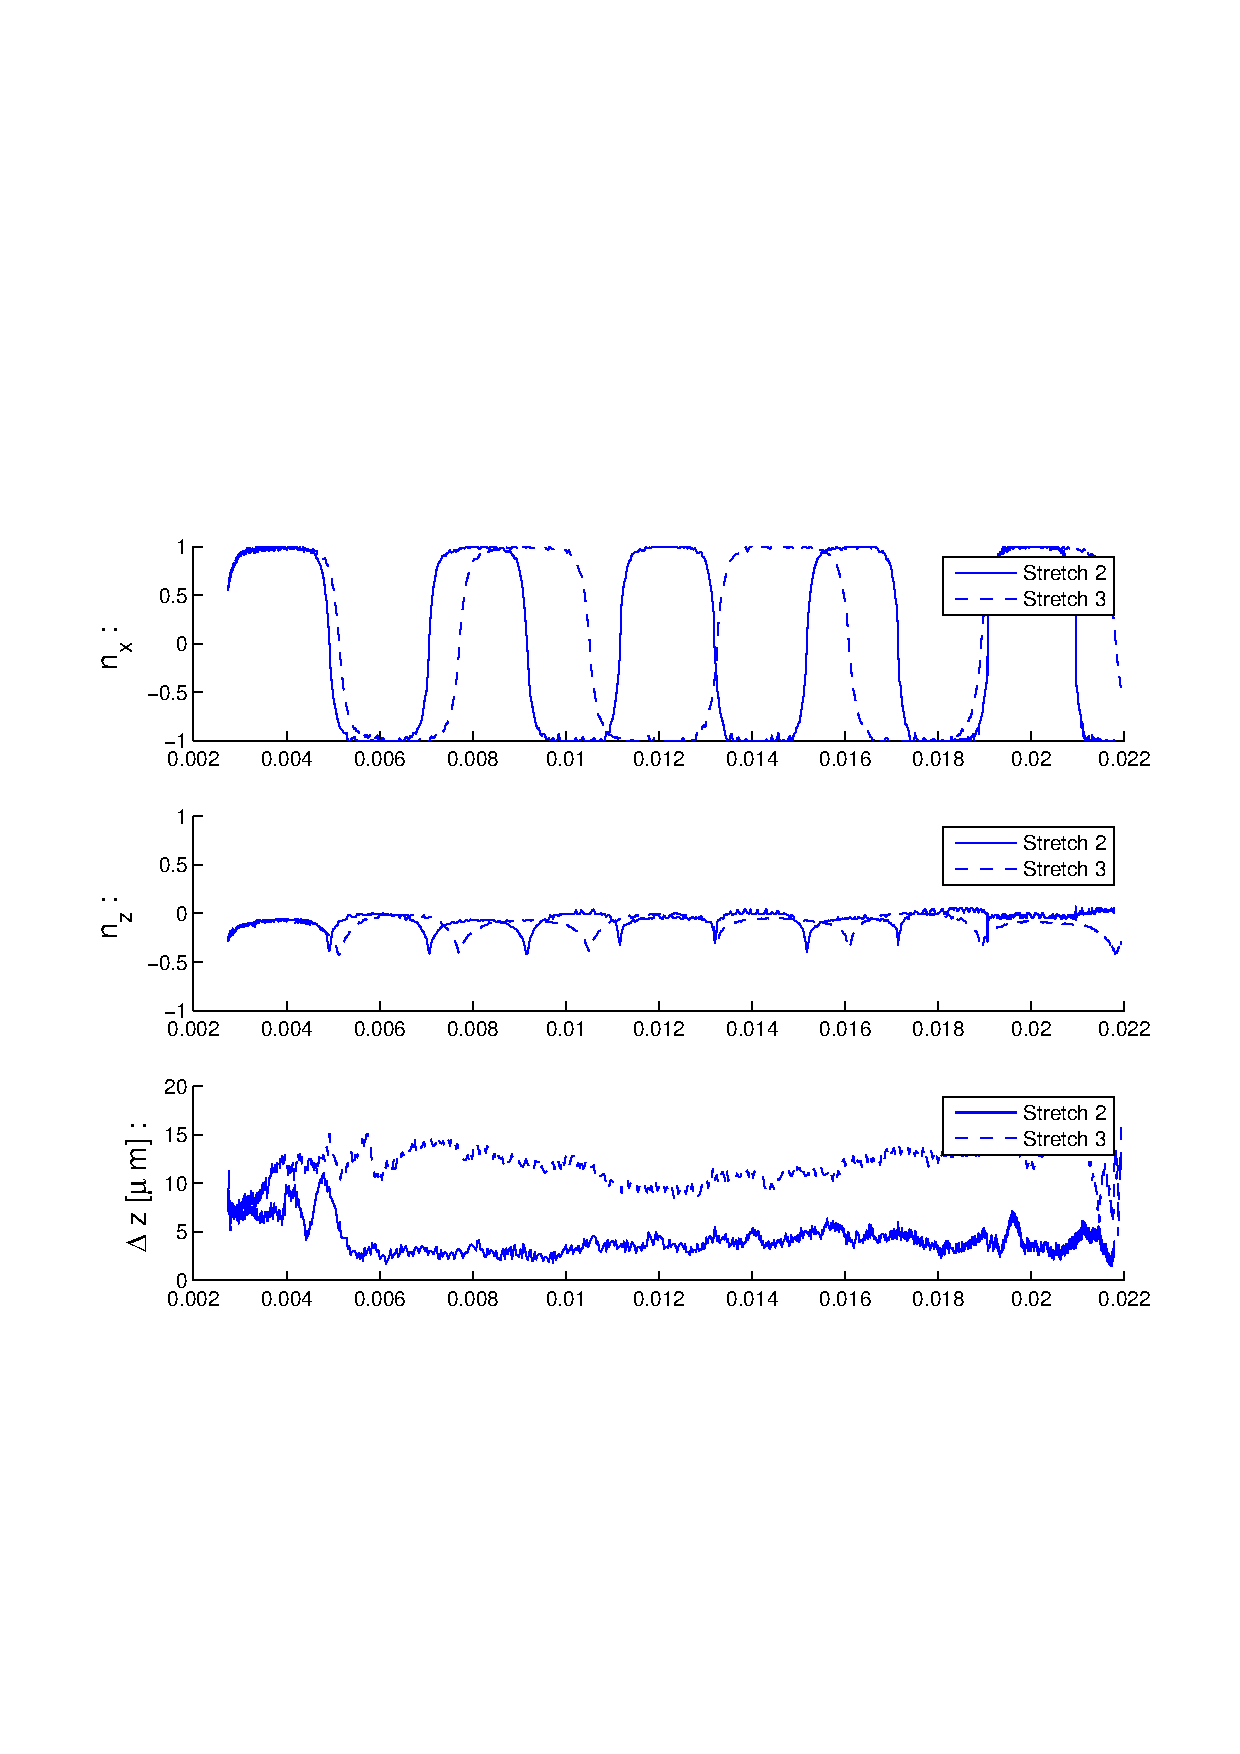
\includegraphics[width=0.8\textwidth]{Images/Particle 1/Stretch2.pdf}

\end{figure}

\subsection{Particle 4}

\begin{figure}[H]
\centering
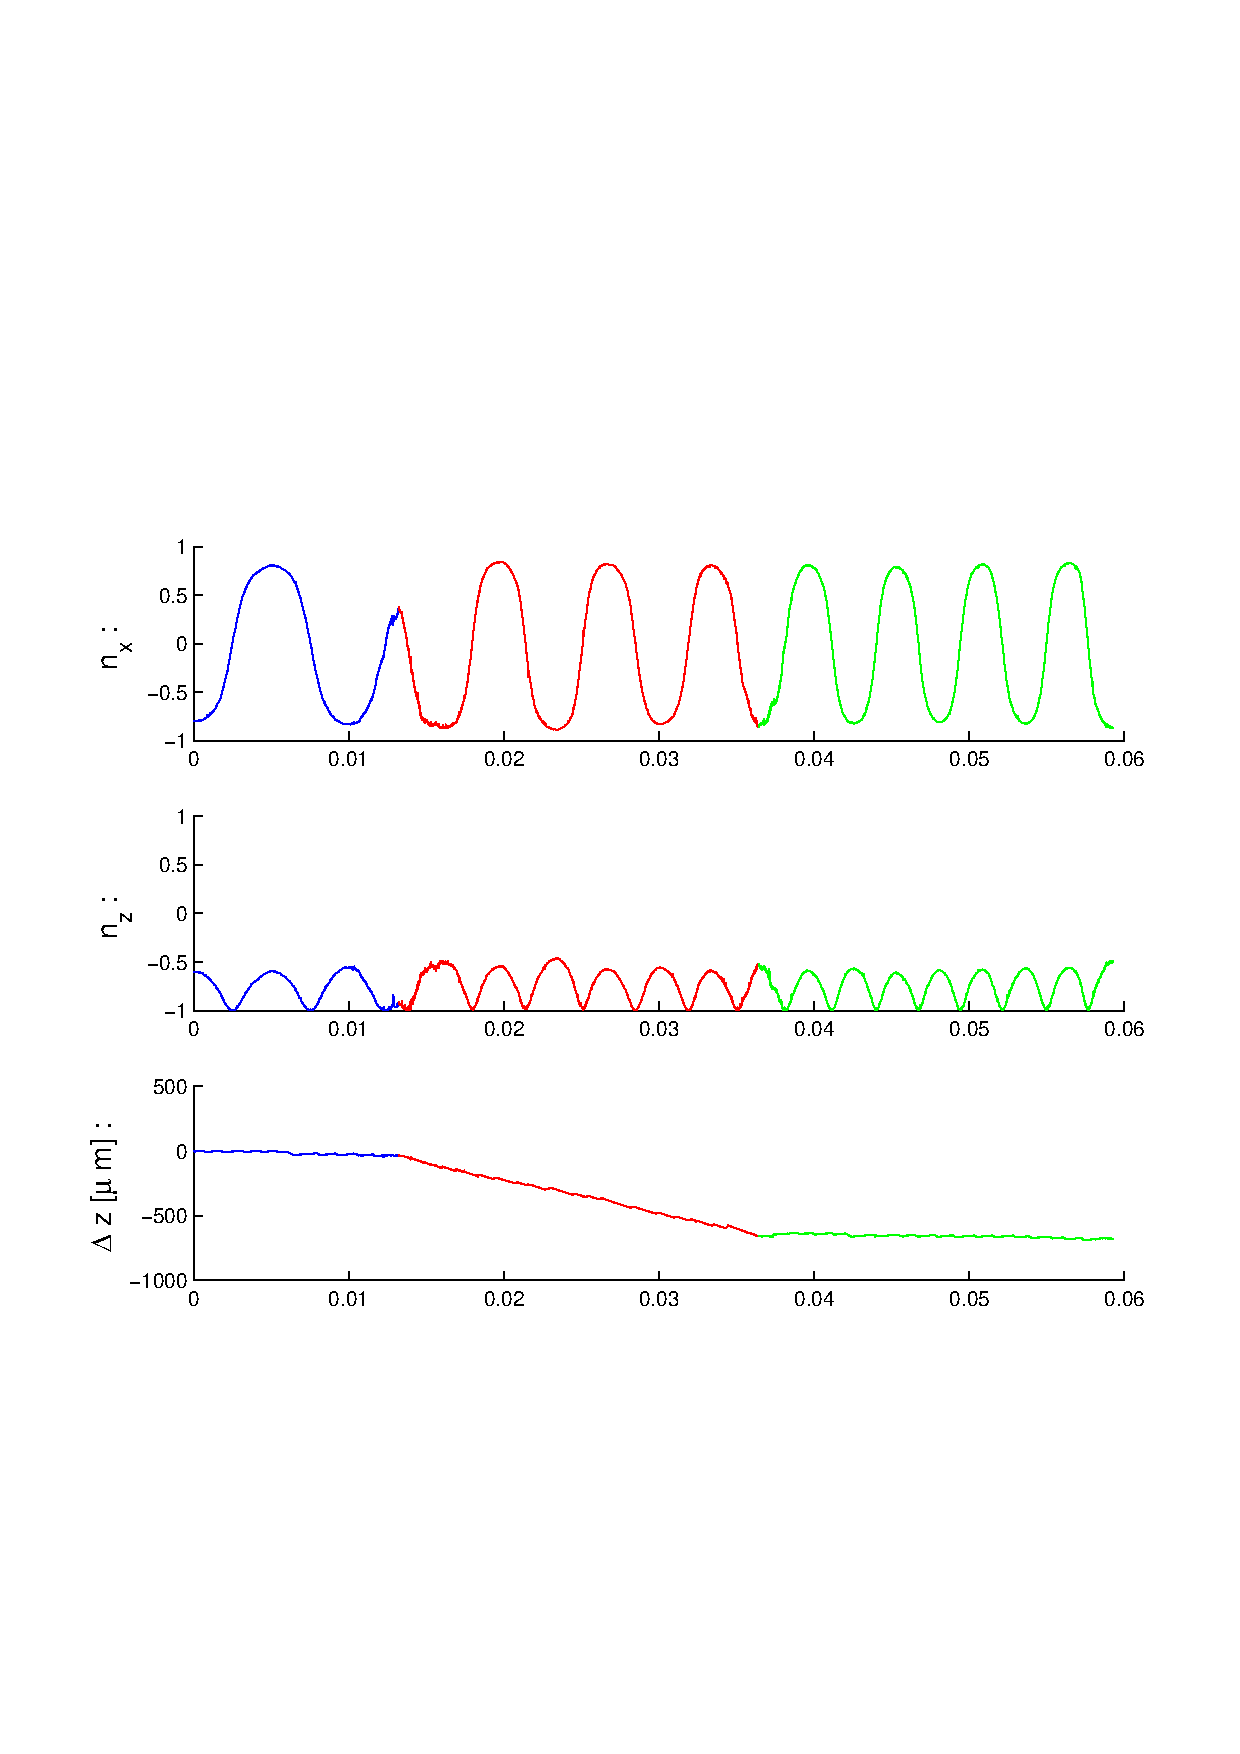
\includegraphics[width=0.8\textwidth]{Images/Particle 4/Particle4.pdf}
\caption{Particle 4: At around 10 minutes, pretty big "jump" in channel flow. $ \lambda: 12.7745$Depth: 140 out of $200 \mu $ m}
\end{figure}

\begin{figure}[H]
\centering
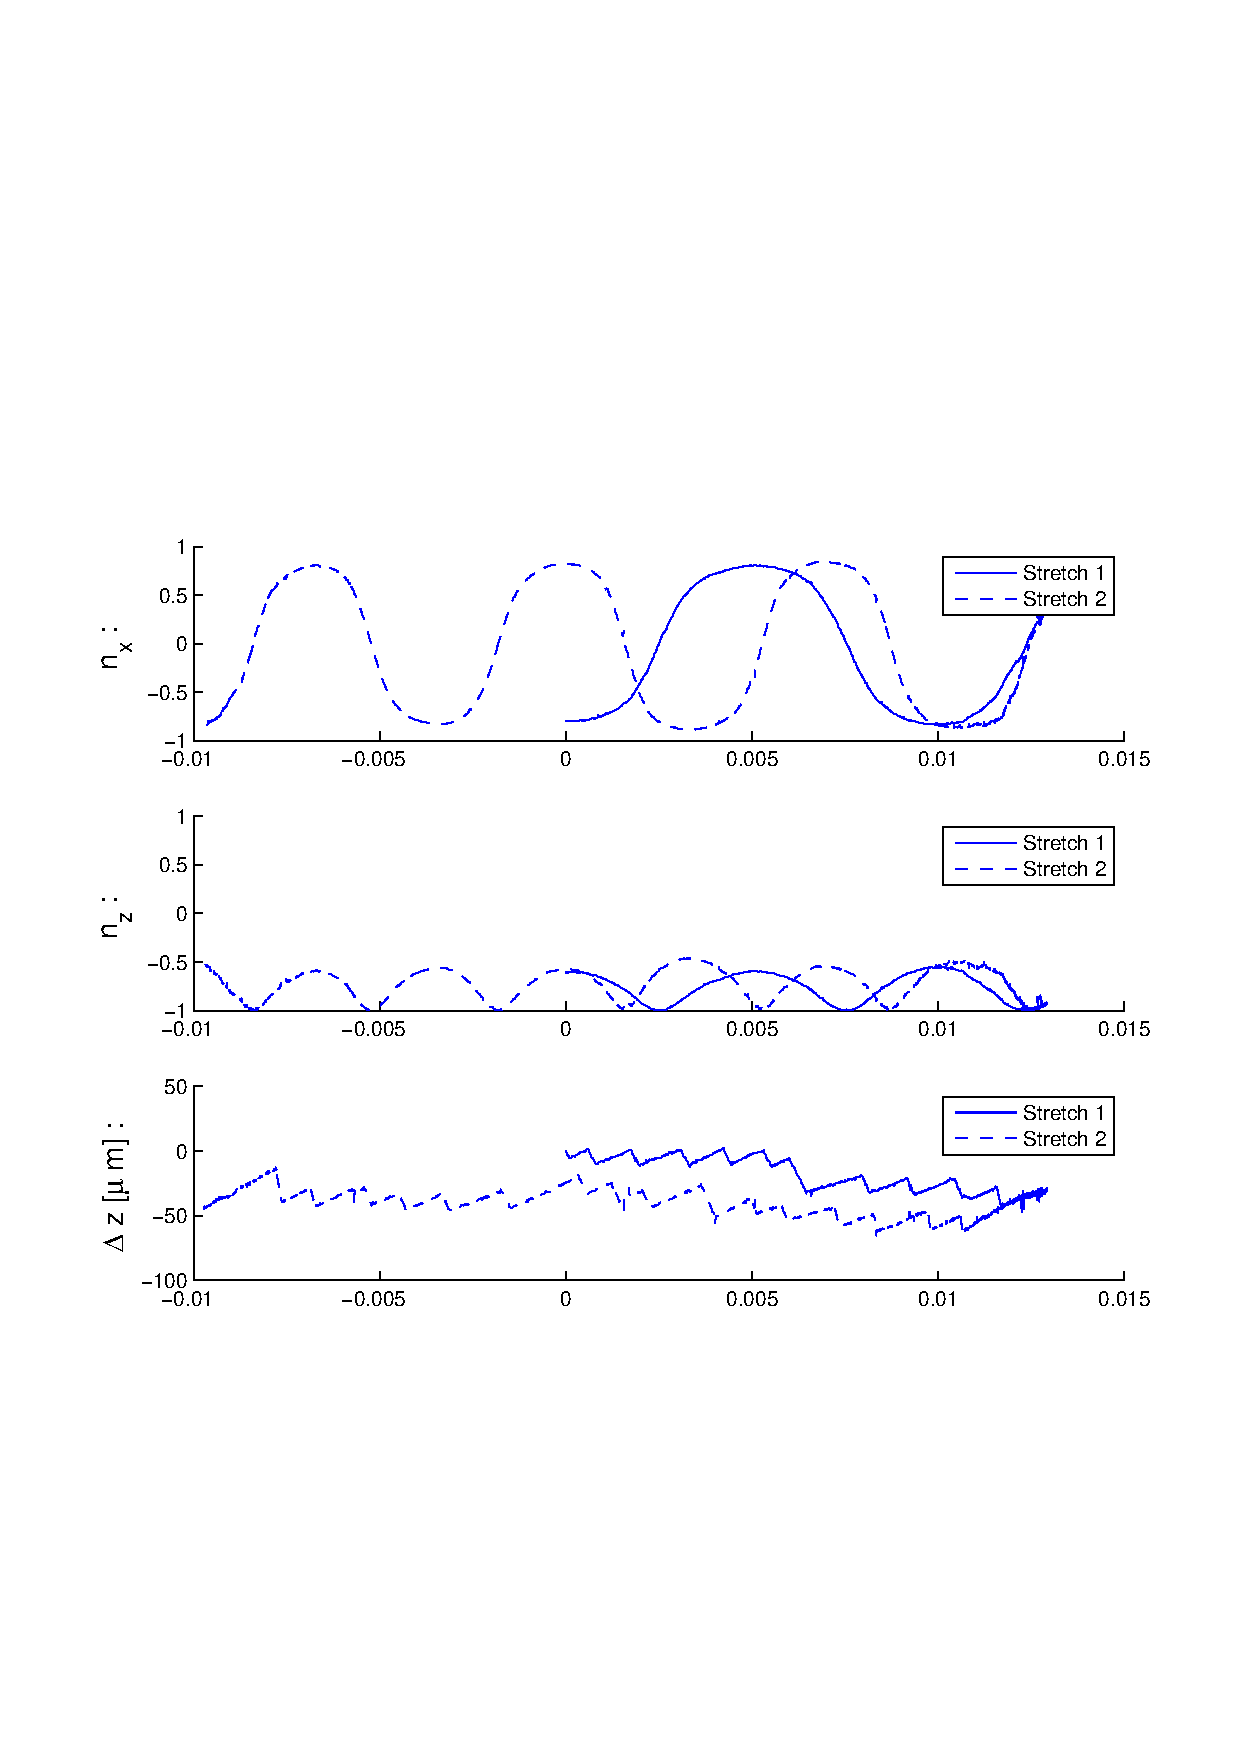
\includegraphics[width=0.8\textwidth]{Images/Particle 4/Stretch1.pdf}
\end{figure}


\begin{figure}[H]
\centering
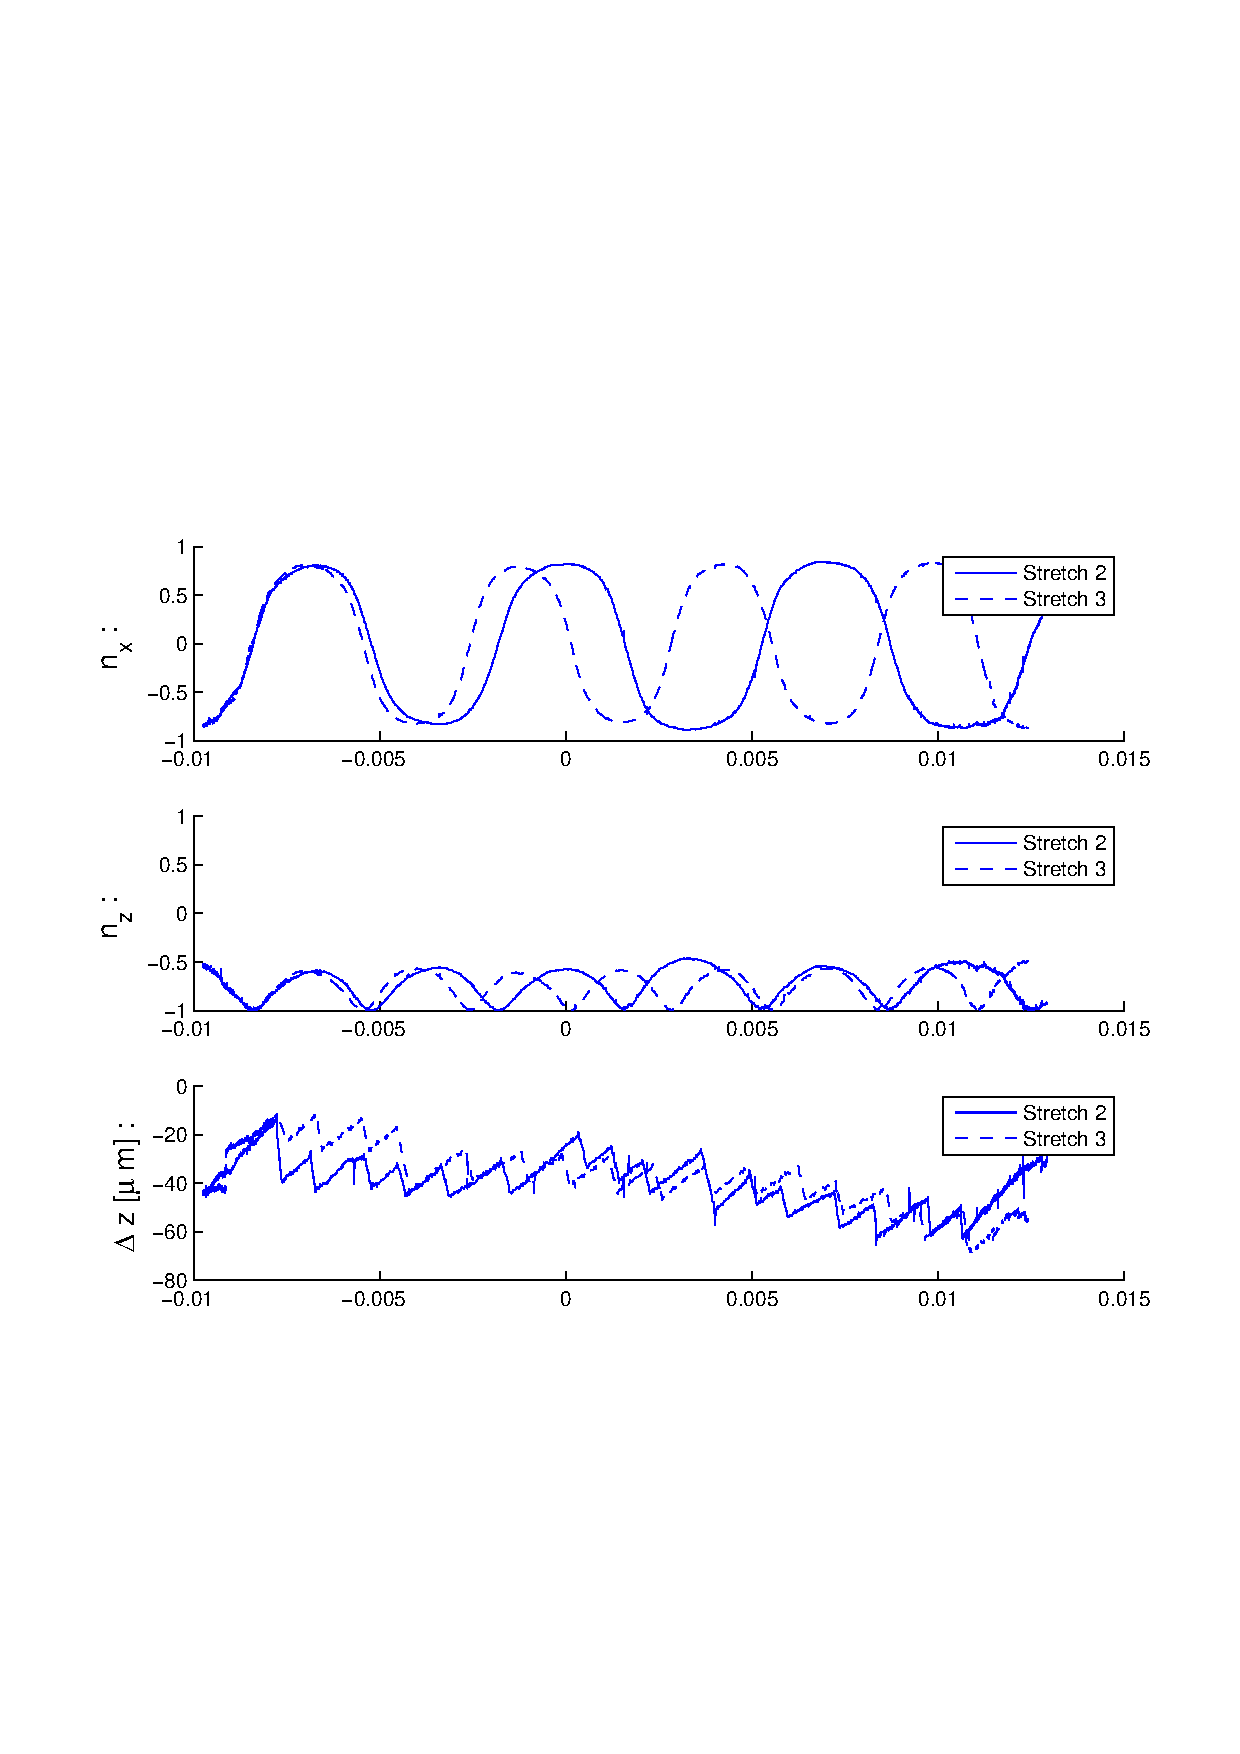
\includegraphics[width=0.8\textwidth]{Images/Particle 4/Stretch2.pdf}
\end{figure}


\subsection{Particle 11}

\begin{figure}[H]
\centering
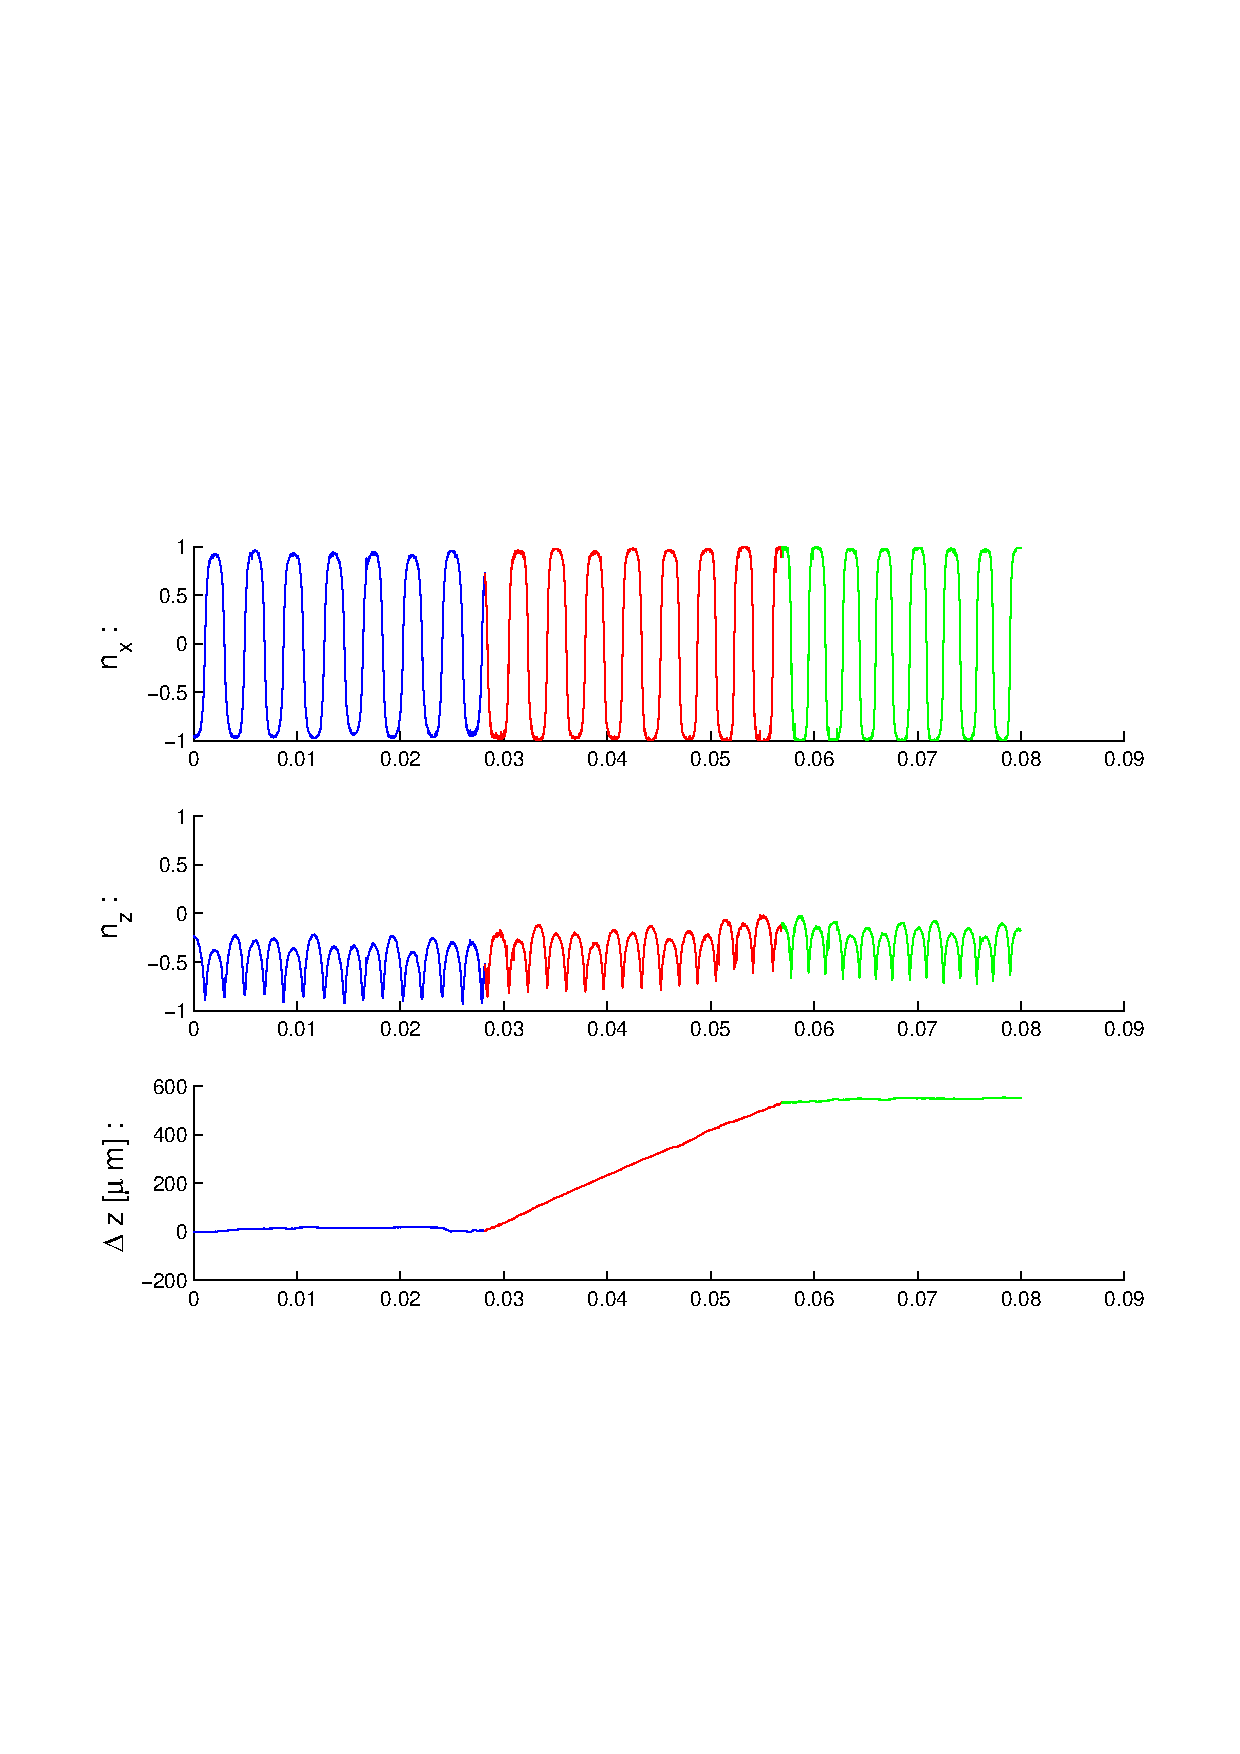
\includegraphics[width=0.8\textwidth]{Images/Particle 11/Particle11.pdf}
\caption{Particle 11: At around 7:03, possible interaction with dirt in channel. $ \lambda: 5.9638$Depth: 180 out of $200 \mu $ m}
\end{figure}

\begin{figure}[H]
\centering
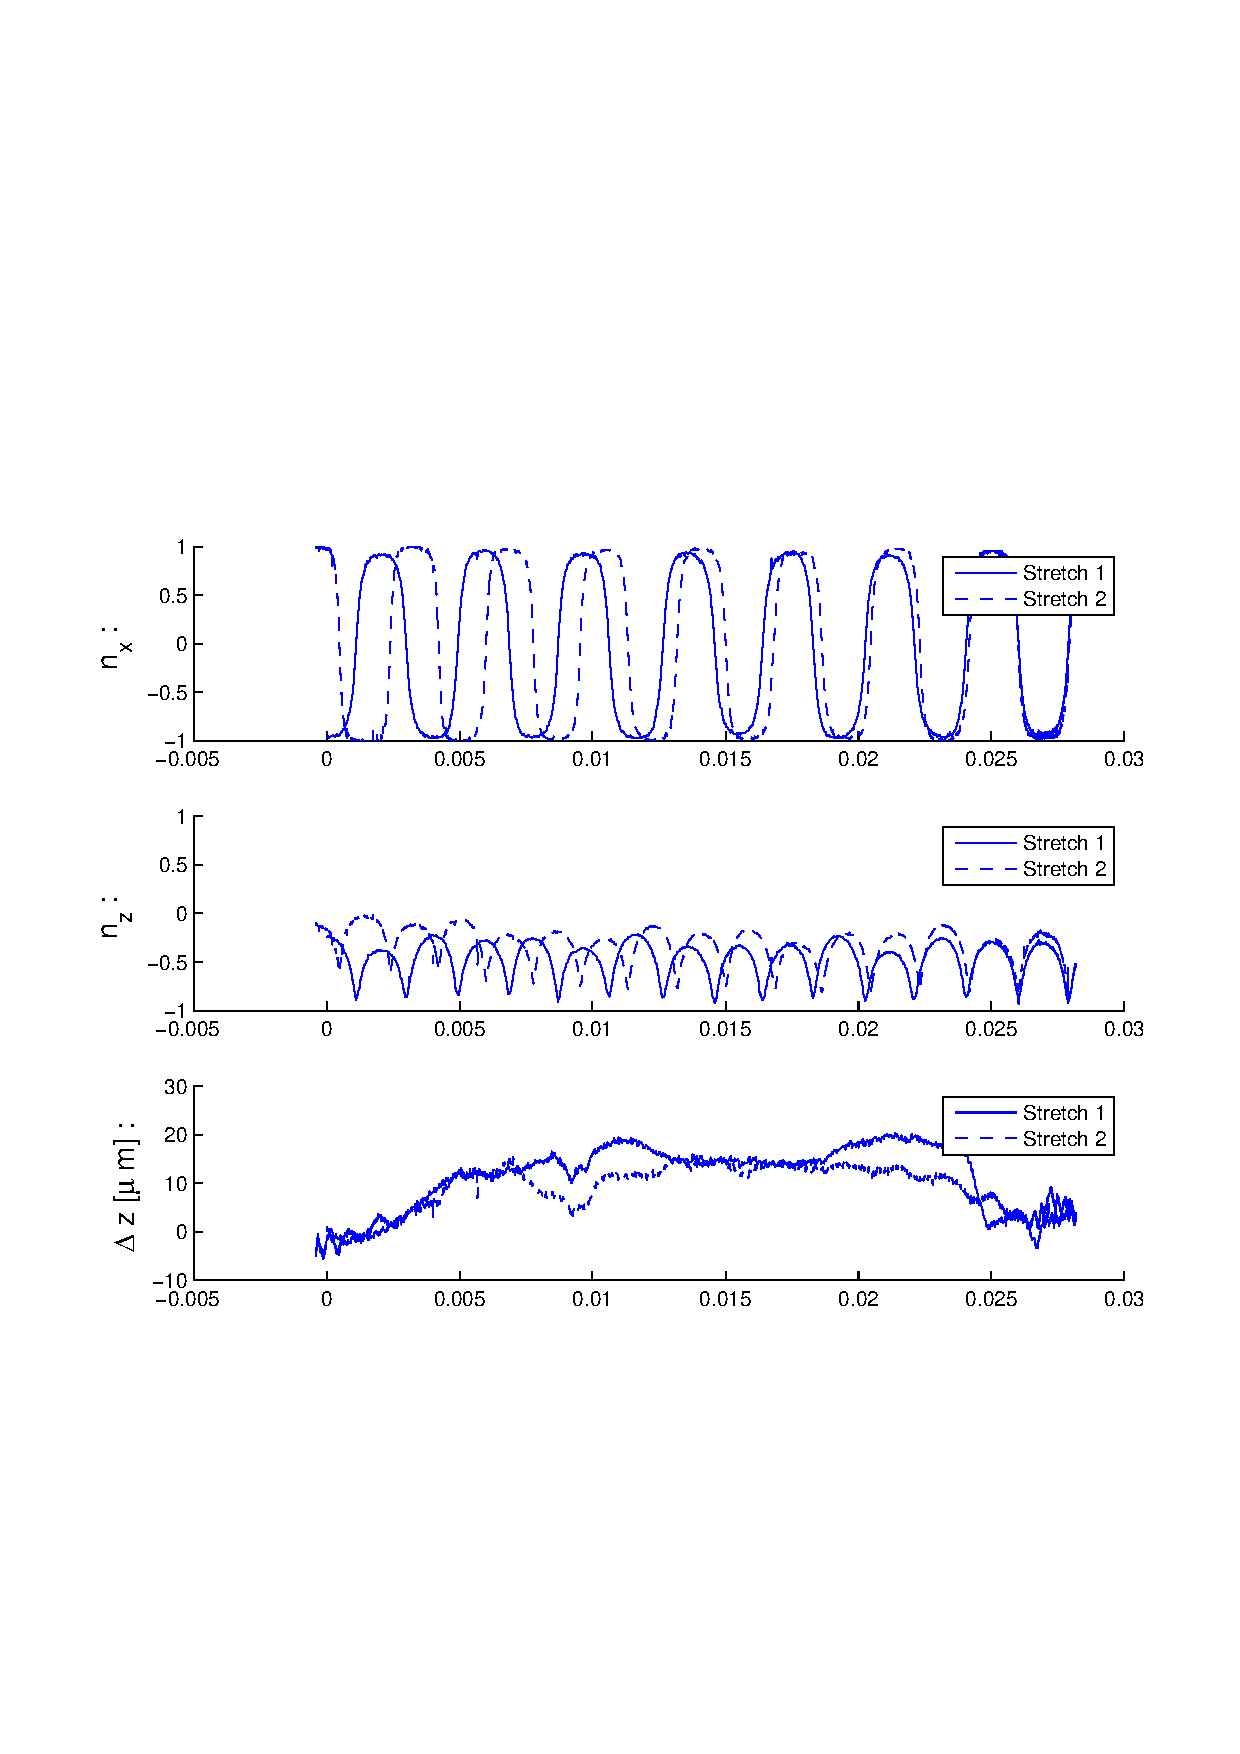
\includegraphics[width=0.8\textwidth]{Images/Particle 11/Stretch1.pdf}
\end{figure}

\begin{figure}[H]
\centering
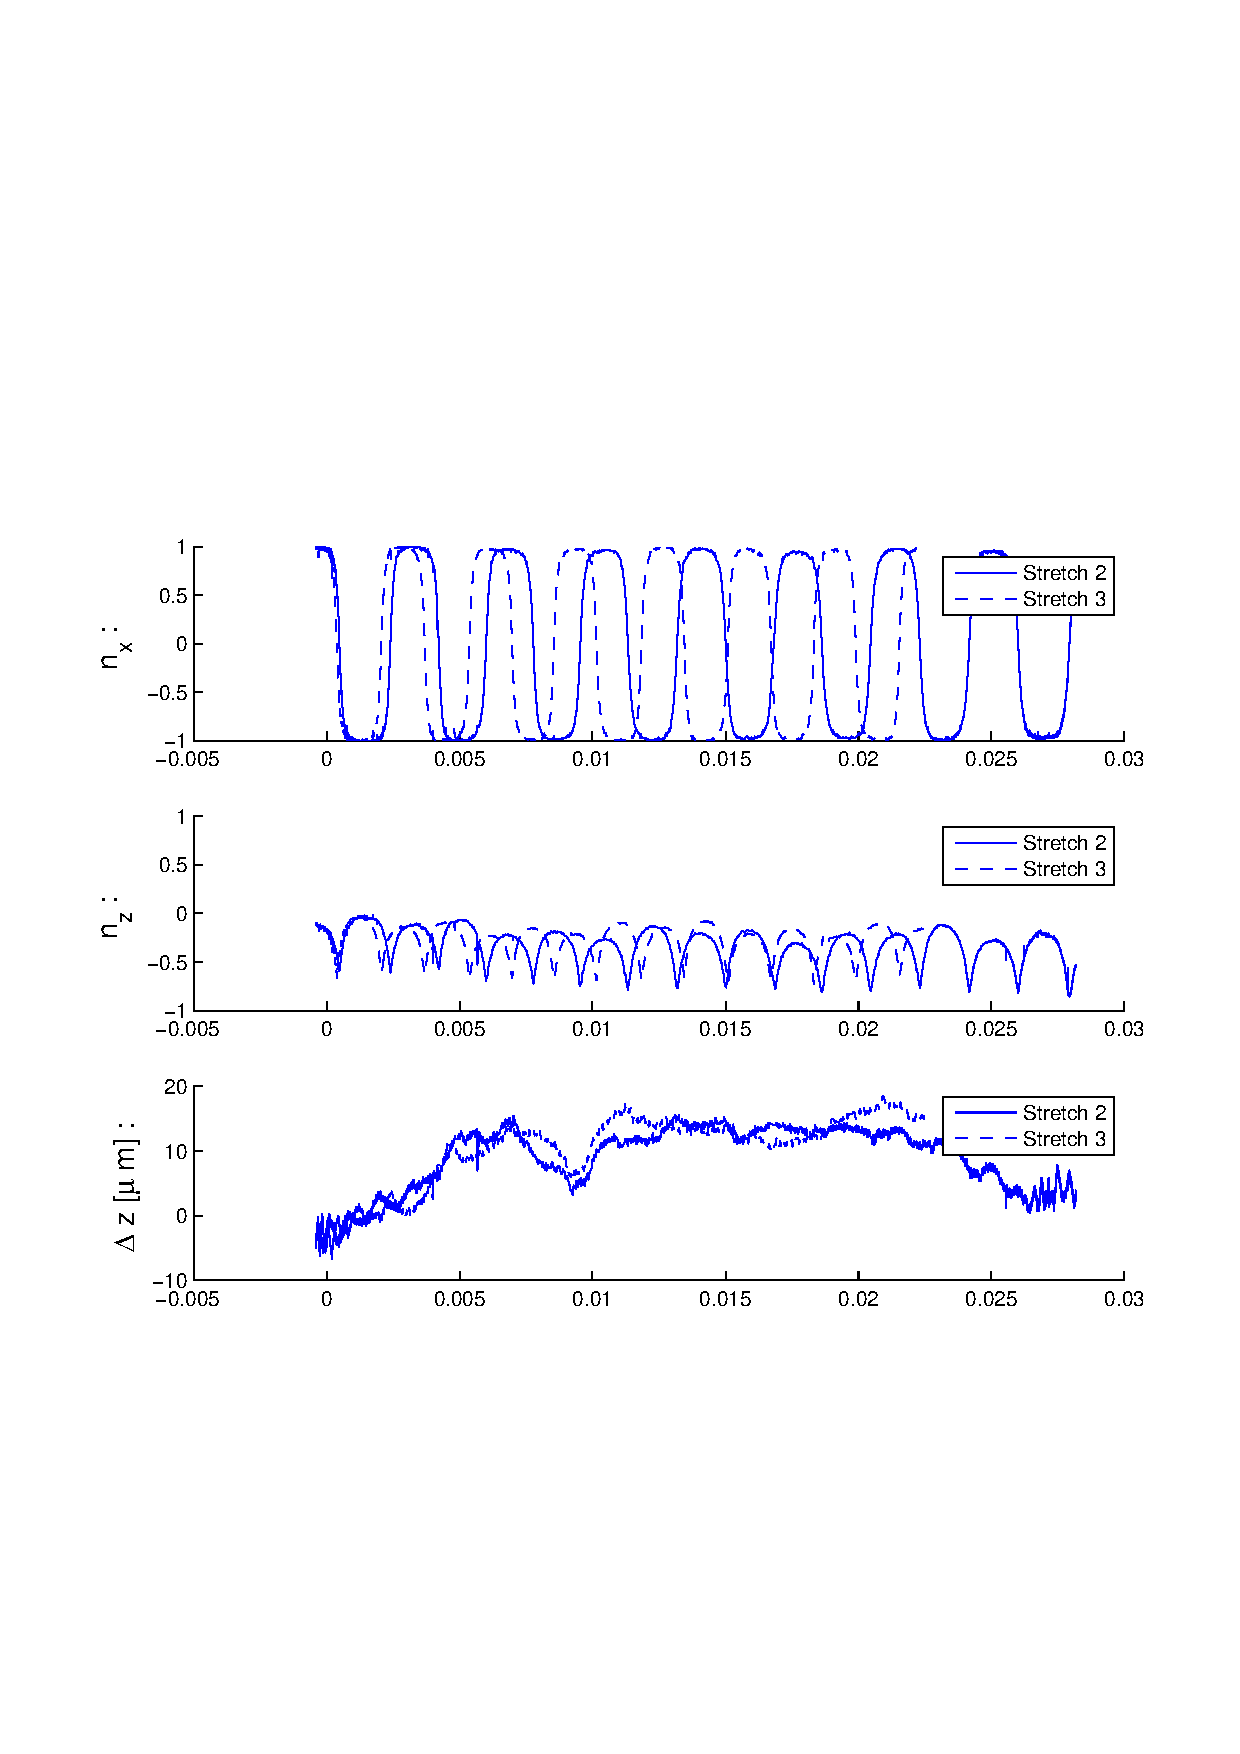
\includegraphics[width=0.8\textwidth]{Images/Particle 11/Stretch2.pdf}
\end{figure}


\subsection{Particle 13}
\begin{figure}[H]
\centering
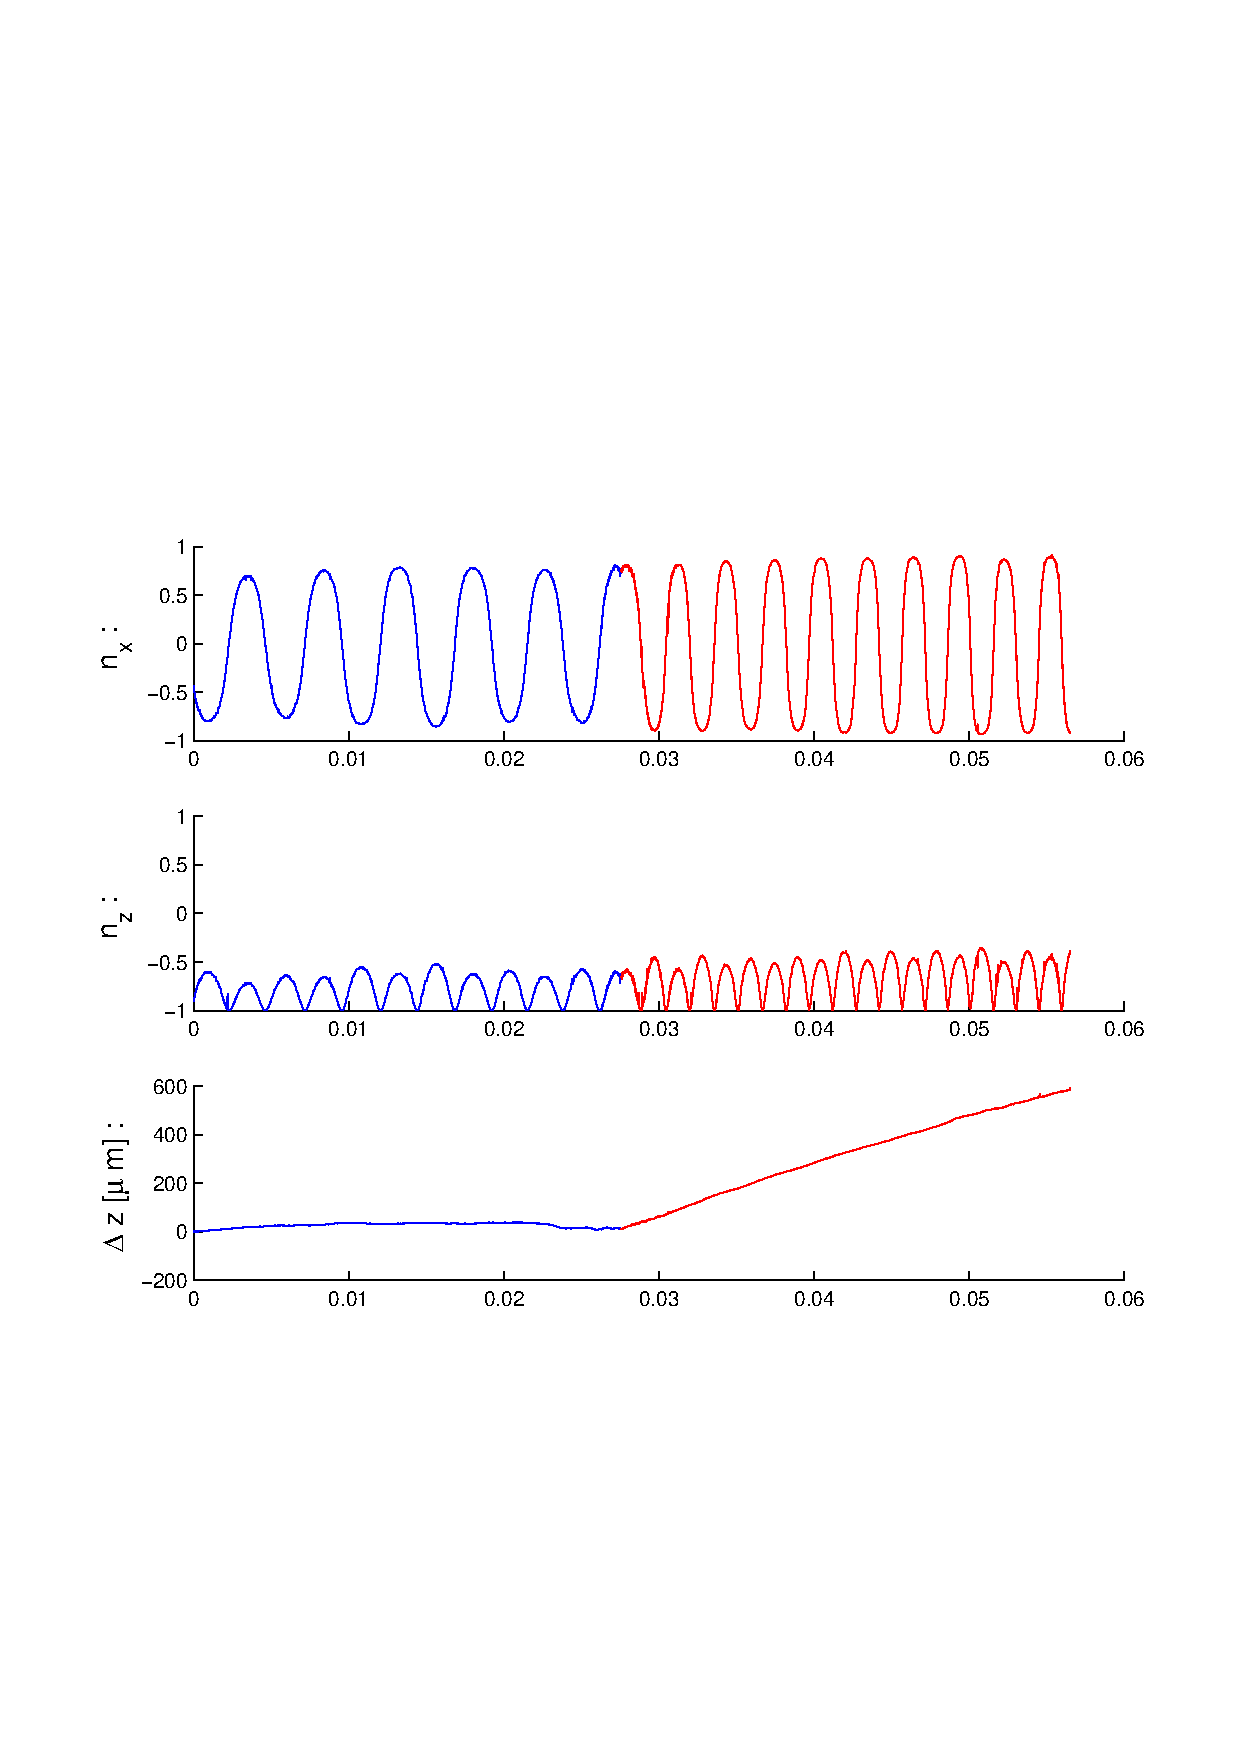
\includegraphics[width=0.8\textwidth]{Images/Particle 13/Particle13.pdf}
\caption{Particle 13: At around 4:15 there is a big jump in the flow at reversal. $ \lambda: 5.5457$Depth: 140 out of $200 \mu $ m}
\end{figure}

\begin{figure}[H]
\centering
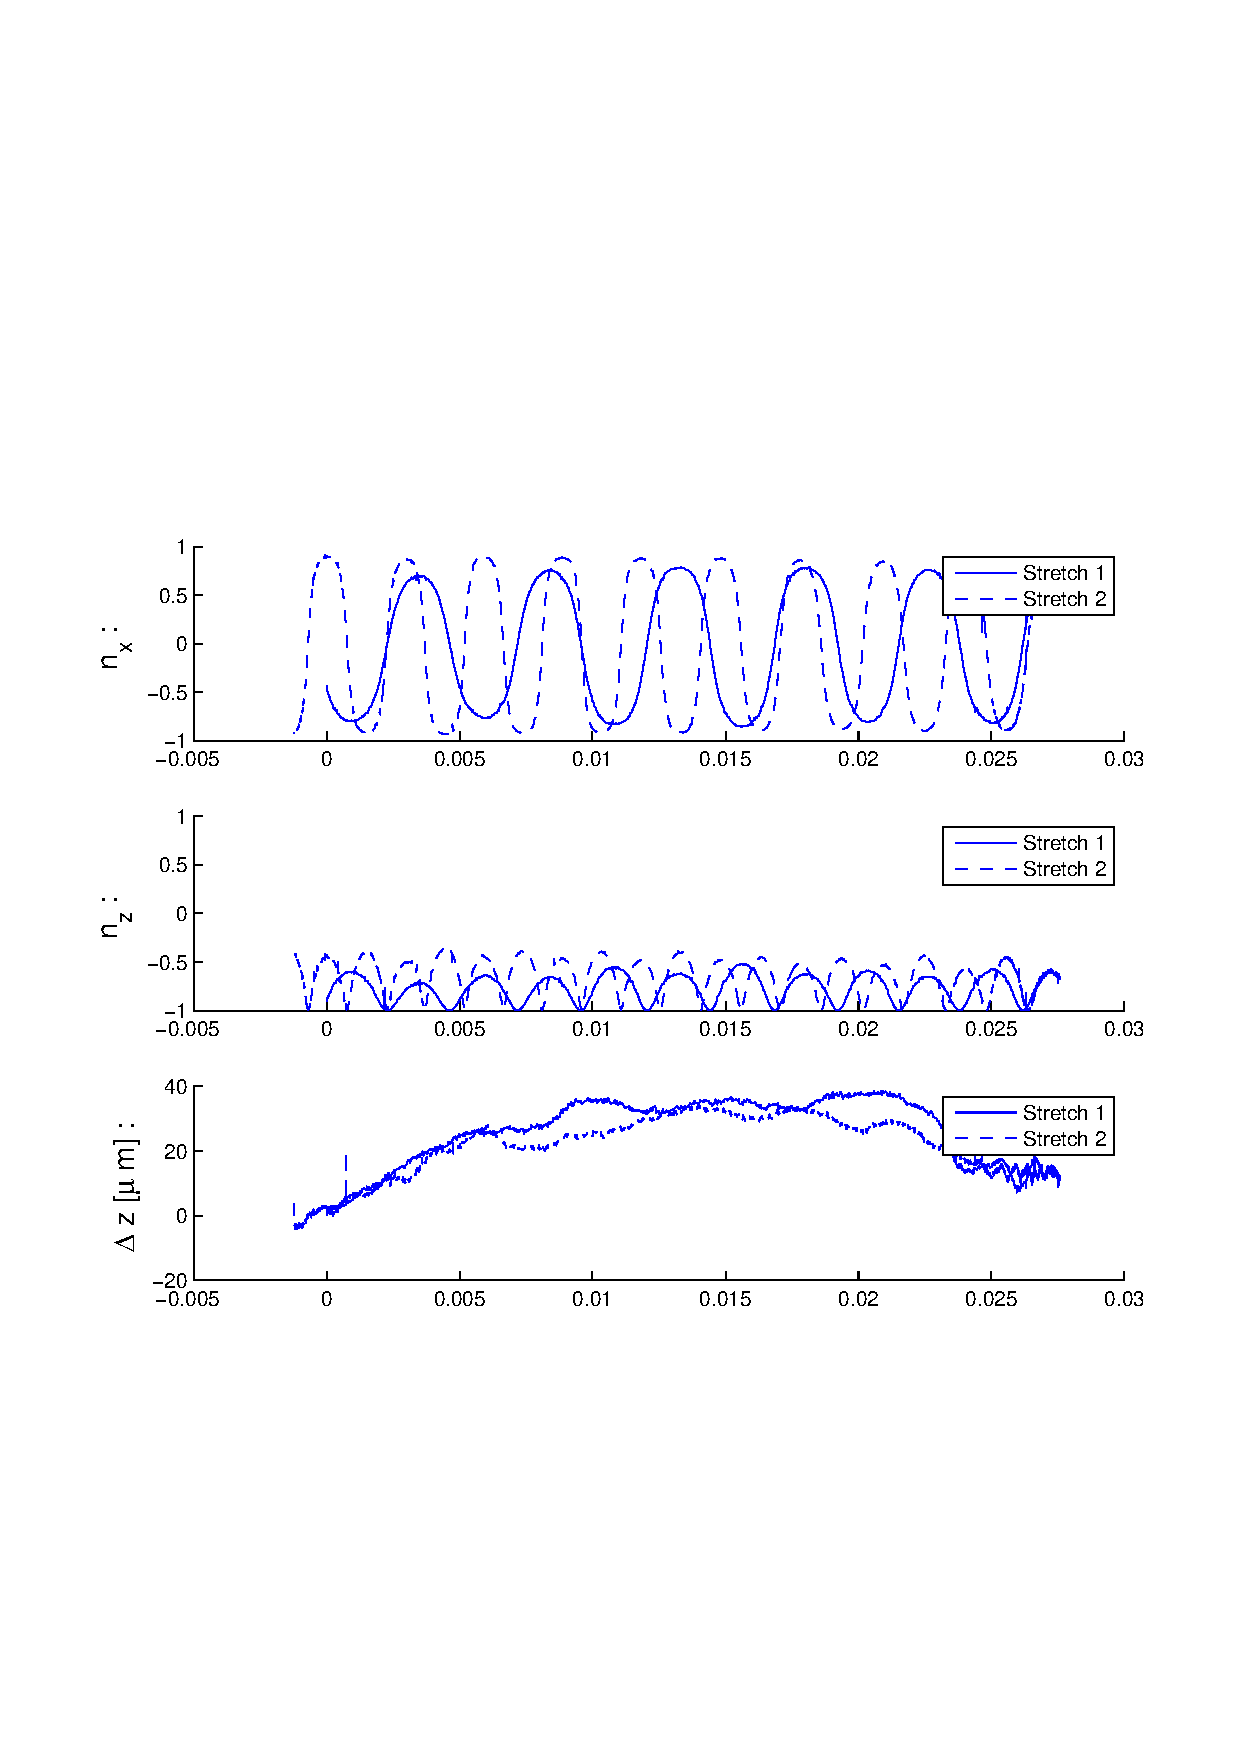
\includegraphics[width=0.8\textwidth]{Images/Particle 13/Stretch1.pdf}
\end{figure}


\subsection{Particle 16}
\begin{figure}[H]
\centering
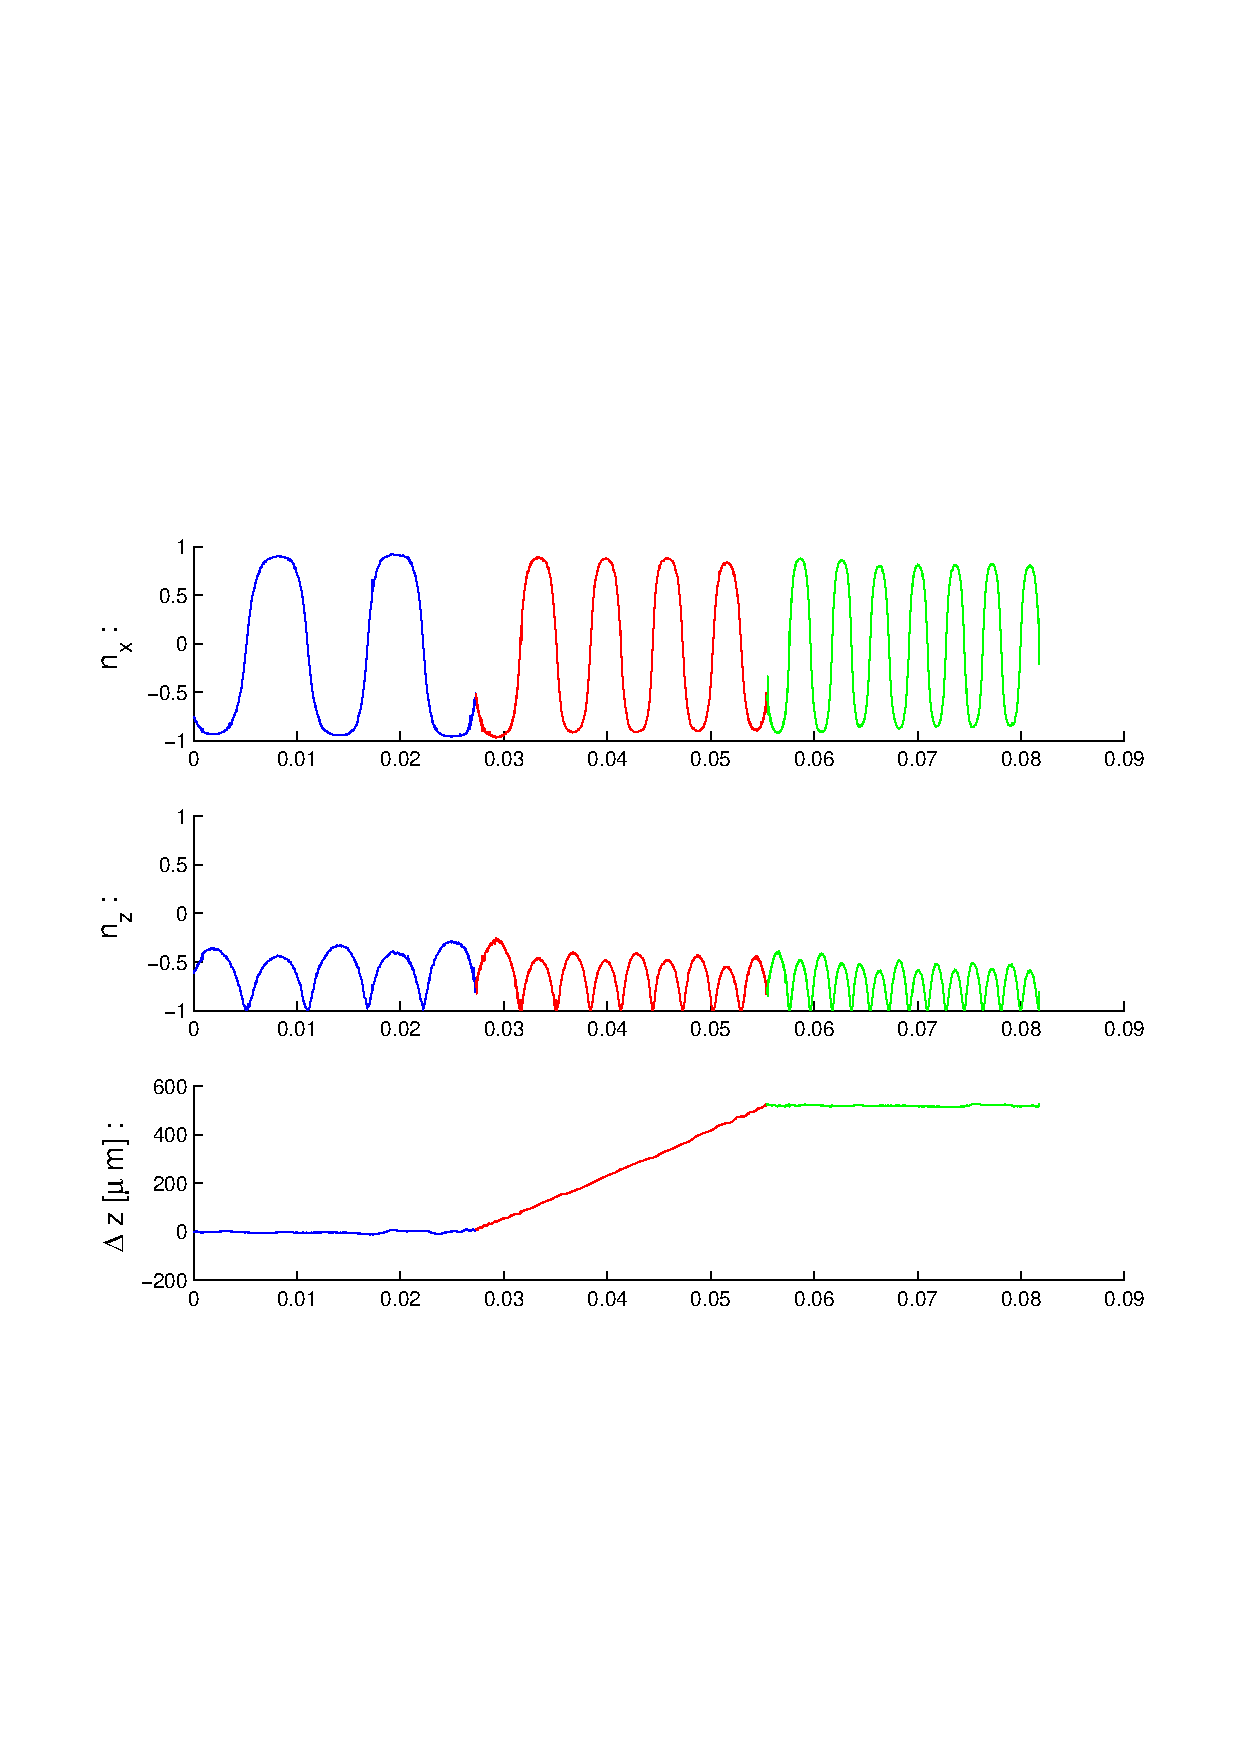
\includegraphics[width=0.8\textwidth]{Images/Particle 16/Particle16.pdf}
\caption{Particle 16: $ \lambda: 6.2917$Depth: 120 out of $200 \mu $ m}
\end{figure}

\begin{figure}[H]

\centering

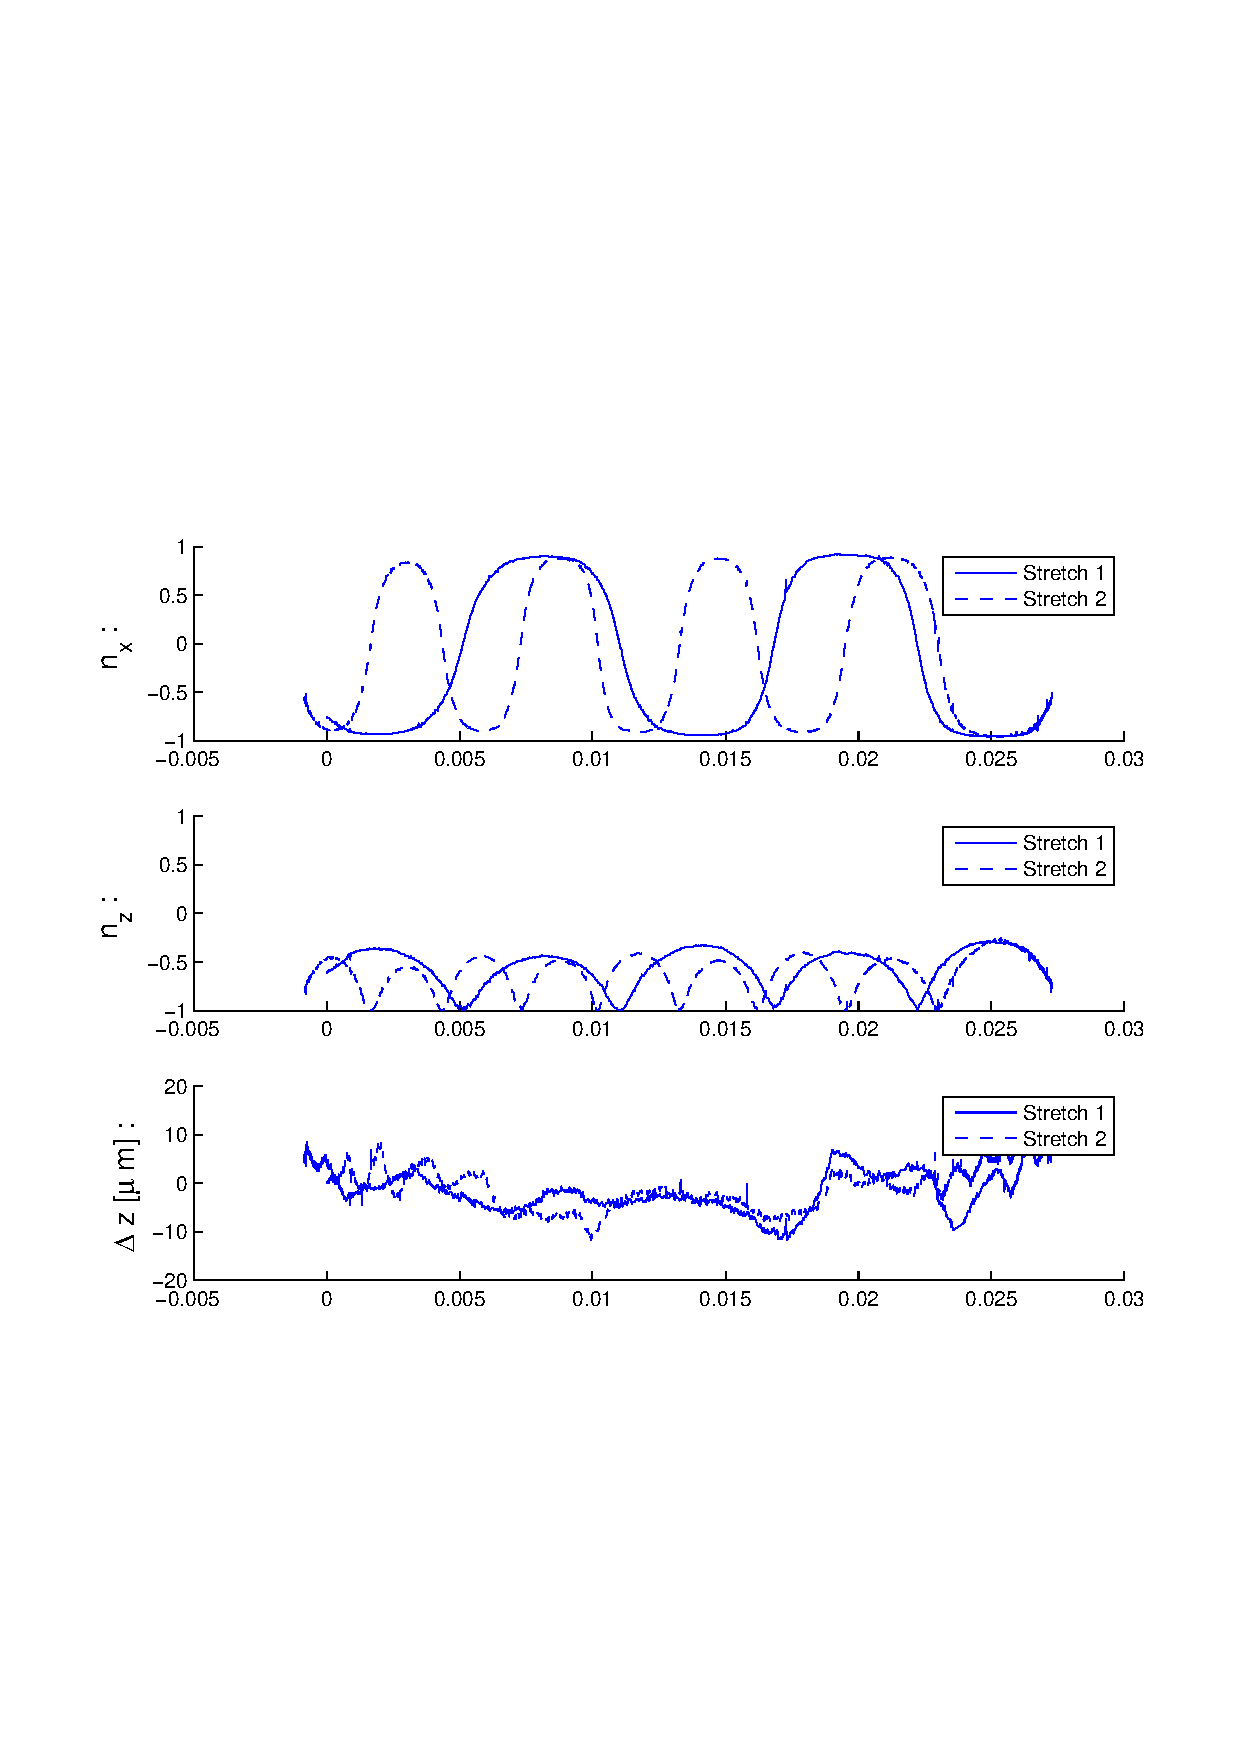
\includegraphics[width=0.8\textwidth]{Images/Particle 16/Stretch1.pdf}

\end{figure}

\begin{figure}[H]

\centering

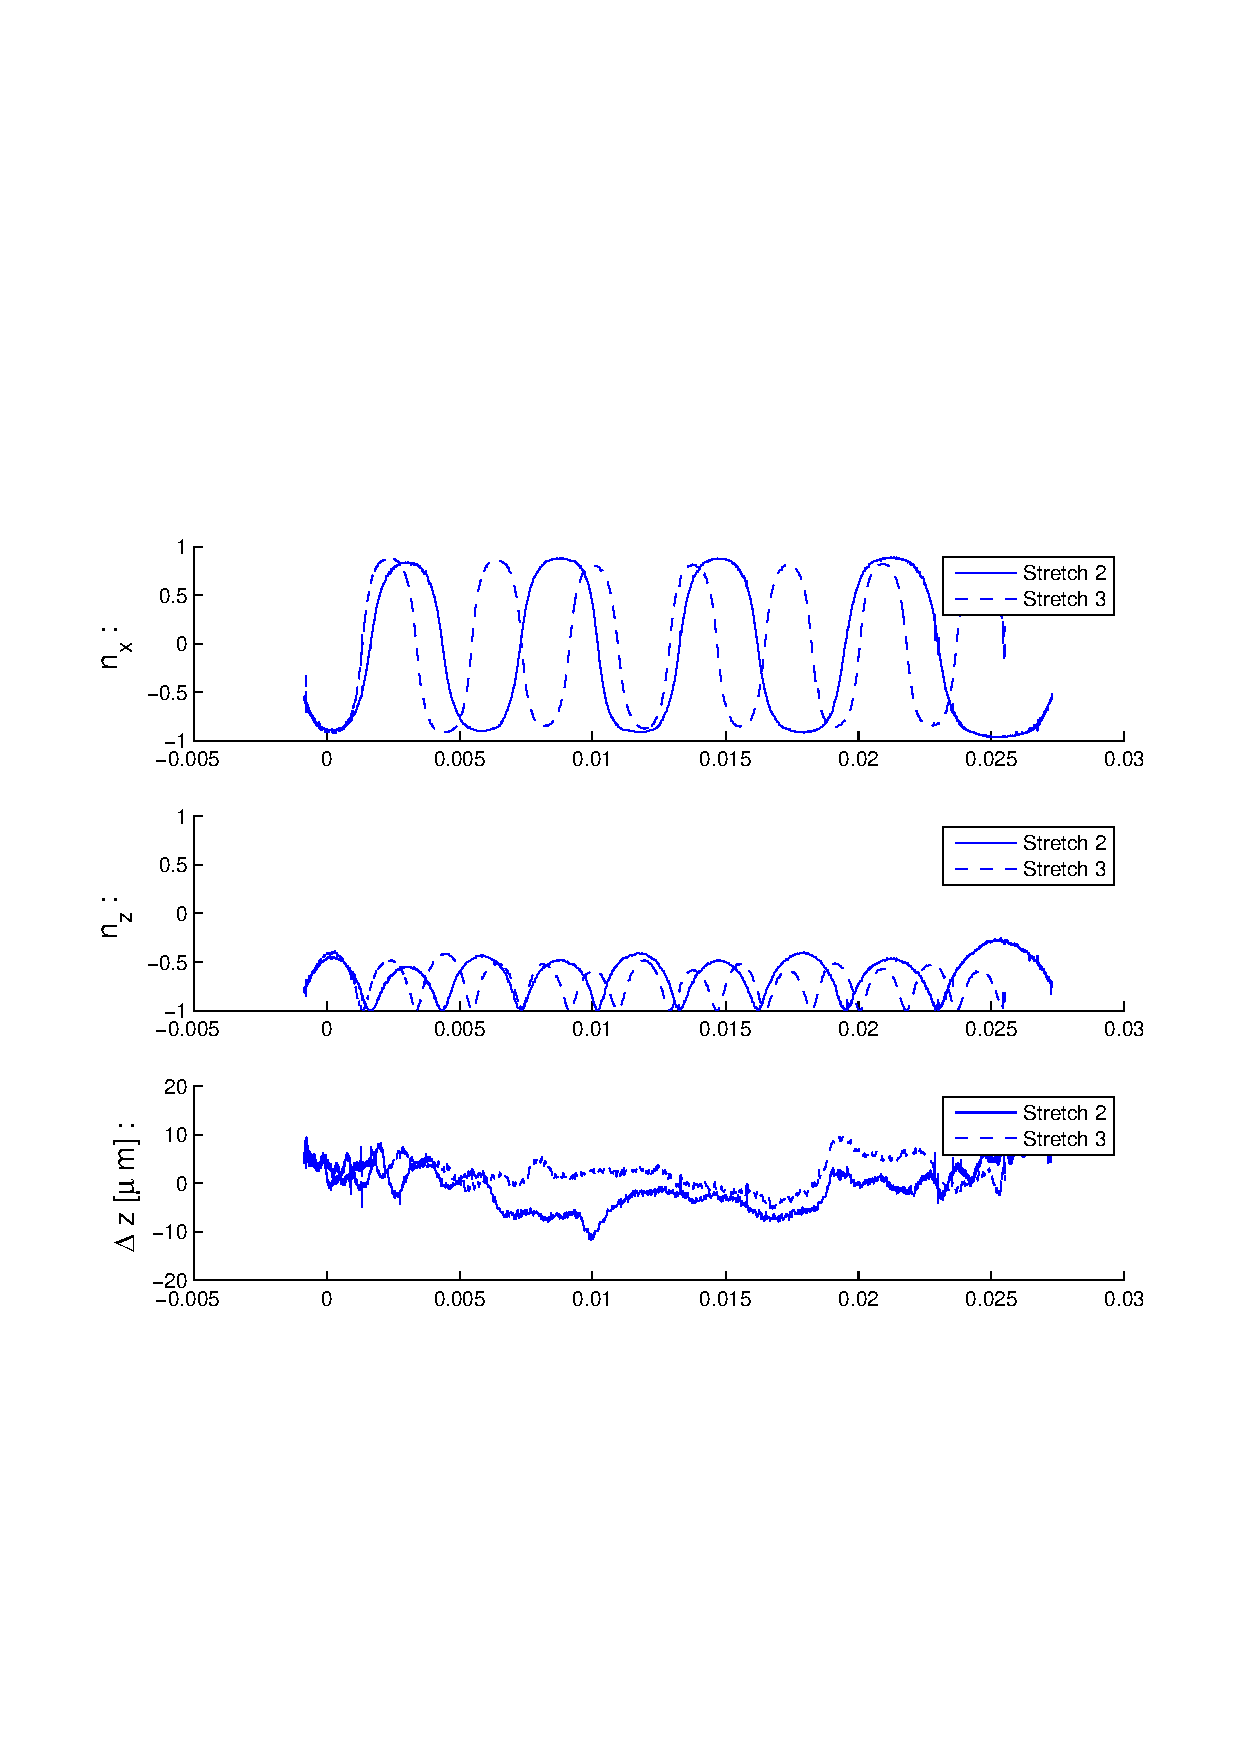
\includegraphics[width=0.8\textwidth]{Images/Particle 16/Stretch2.pdf}

\end{figure}



\subsection{Particle 22}

\begin{figure}[H]


\centering
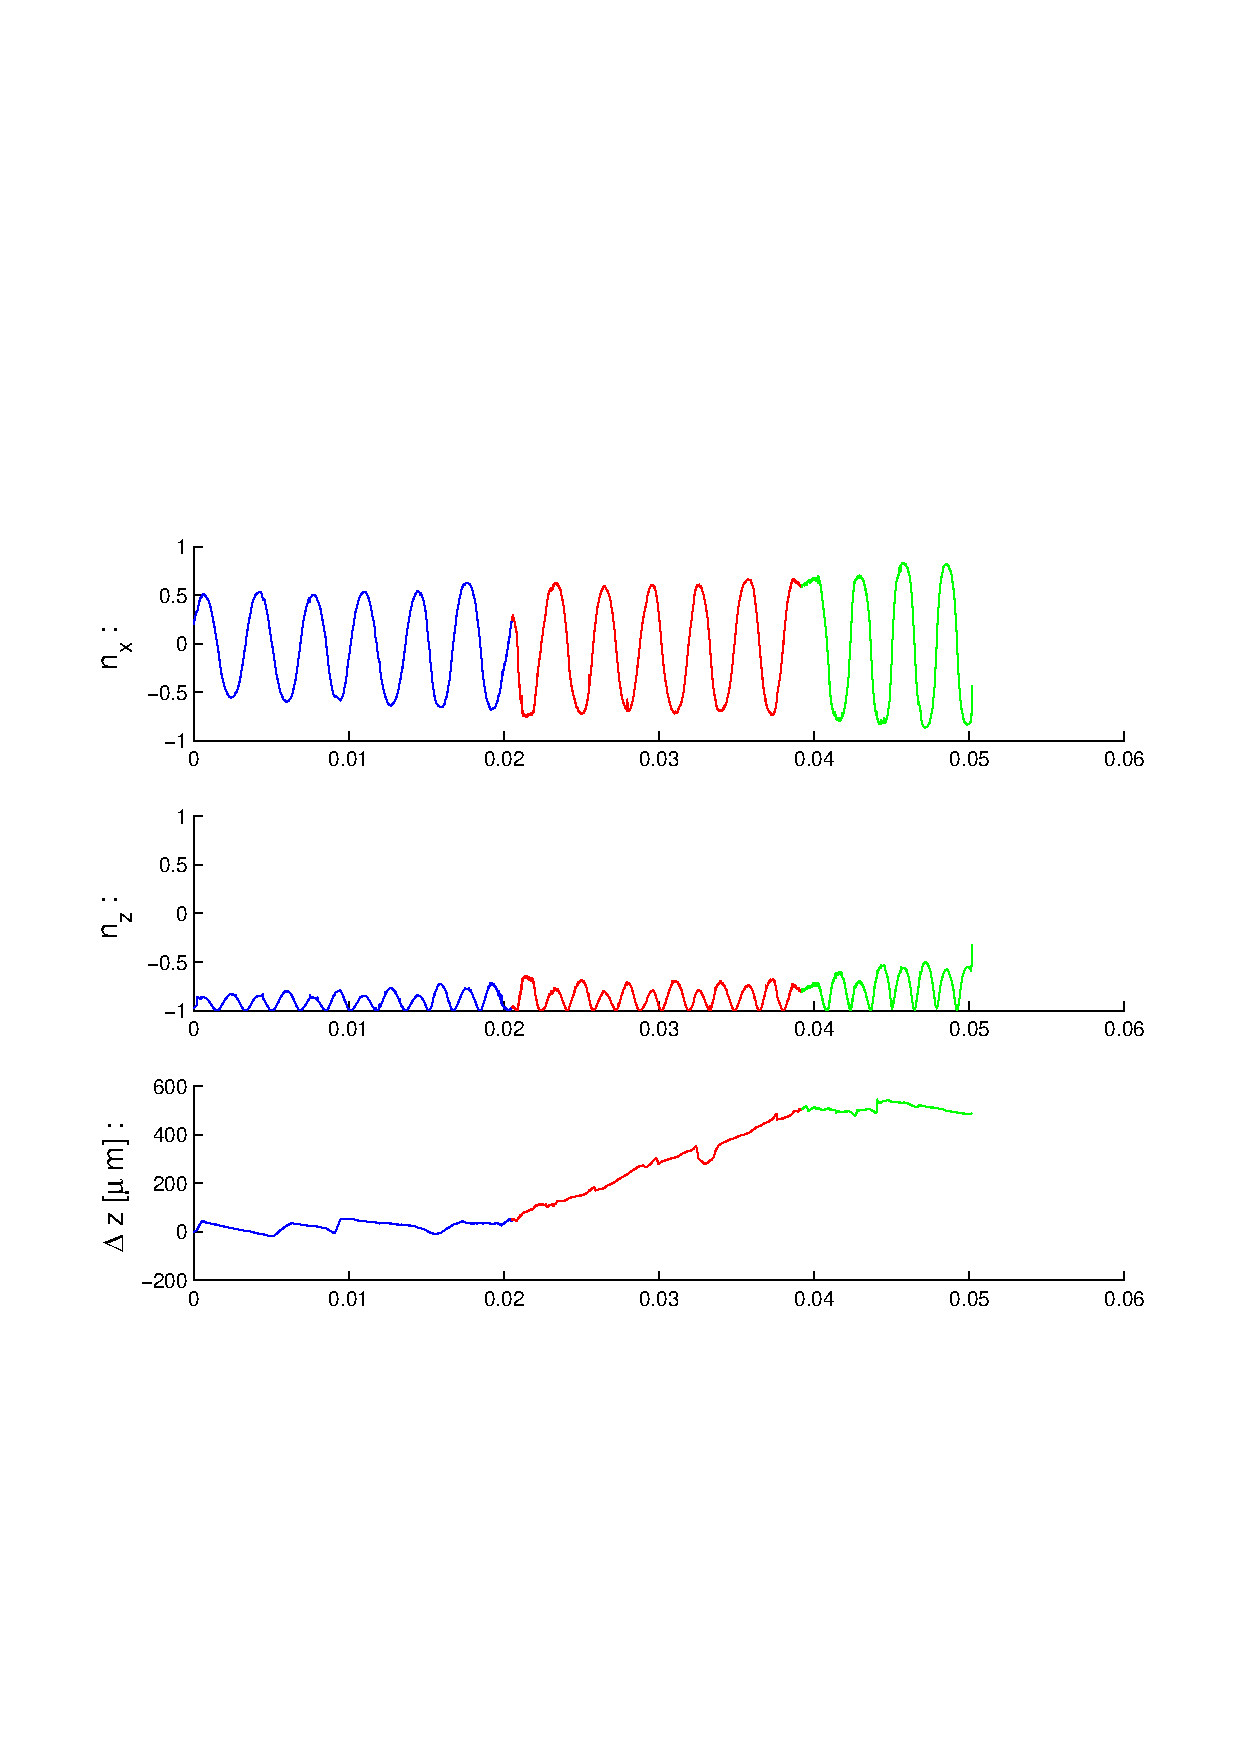
\includegraphics[width=0.8\textwidth]{Images/Particle 22/Particle22.pdf}
\caption{Particle 22: $ \lambda: 11.6767$Depth: 160 out of $200 \mu $ m}

\end{figure}

\begin{figure}[H]

\centering

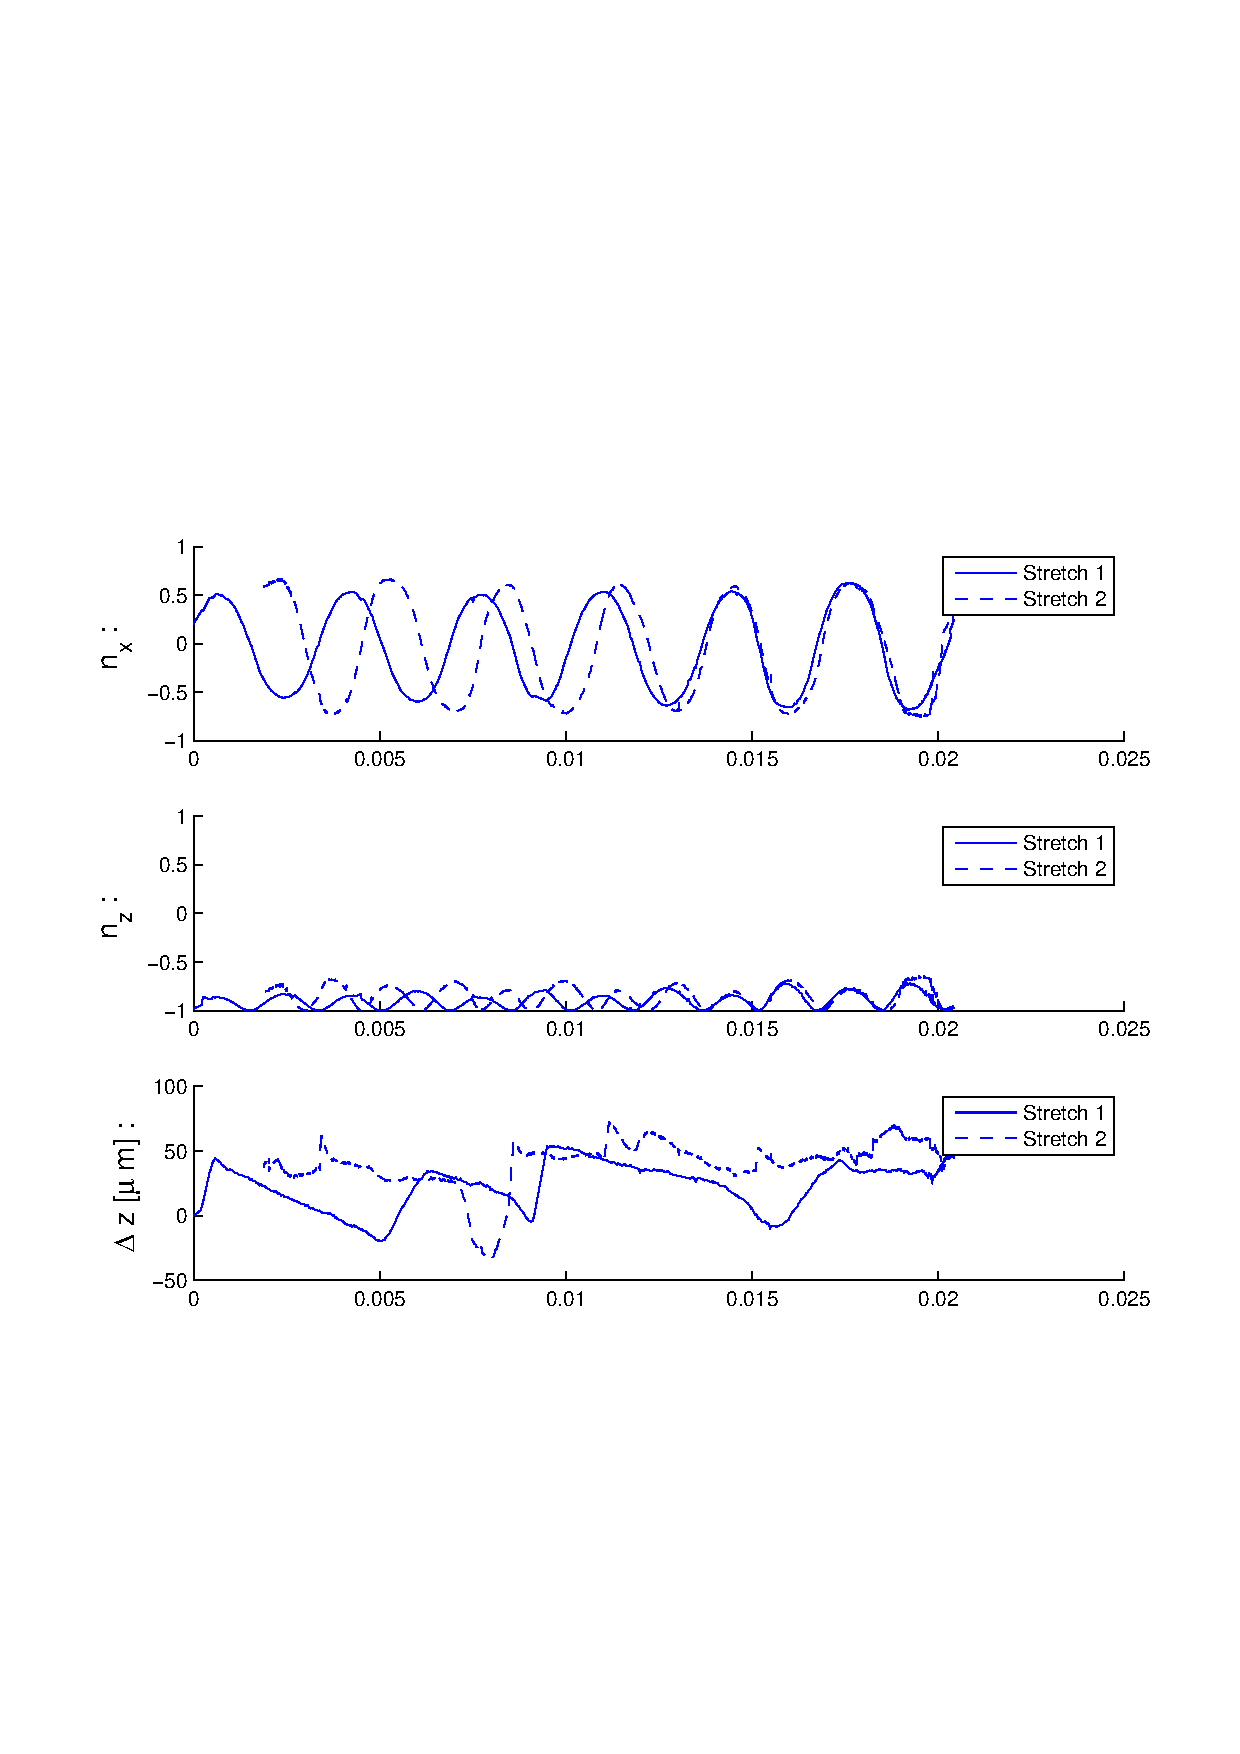
\includegraphics[width=0.8\textwidth]{Images/Particle 22/Stretch1.pdf}

\end{figure}

\begin{figure}[H]

\centering

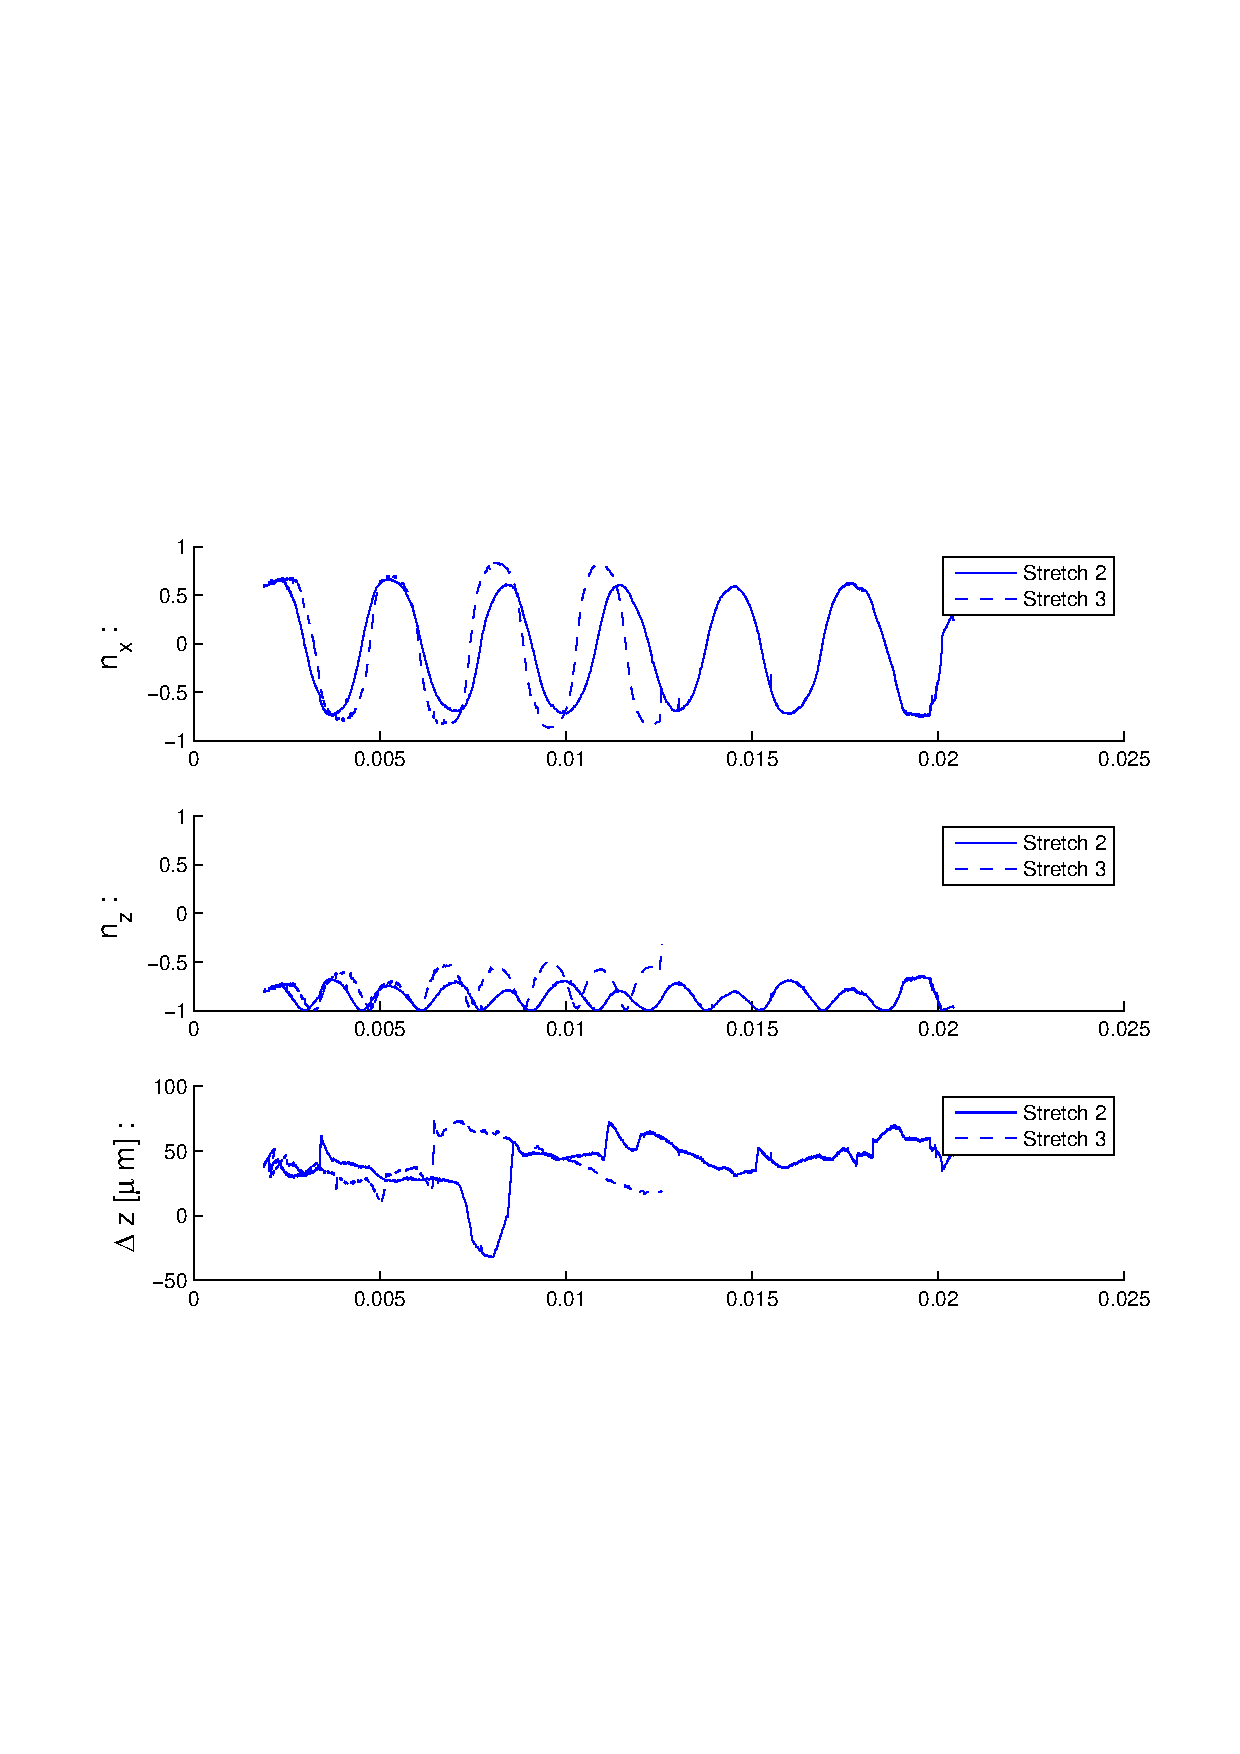
\includegraphics[width=0.8\textwidth]{Images/Particle 22/Stretch2.pdf}

\end{figure}

\subsection{Particle 23}

\begin{figure}[H]
\centering
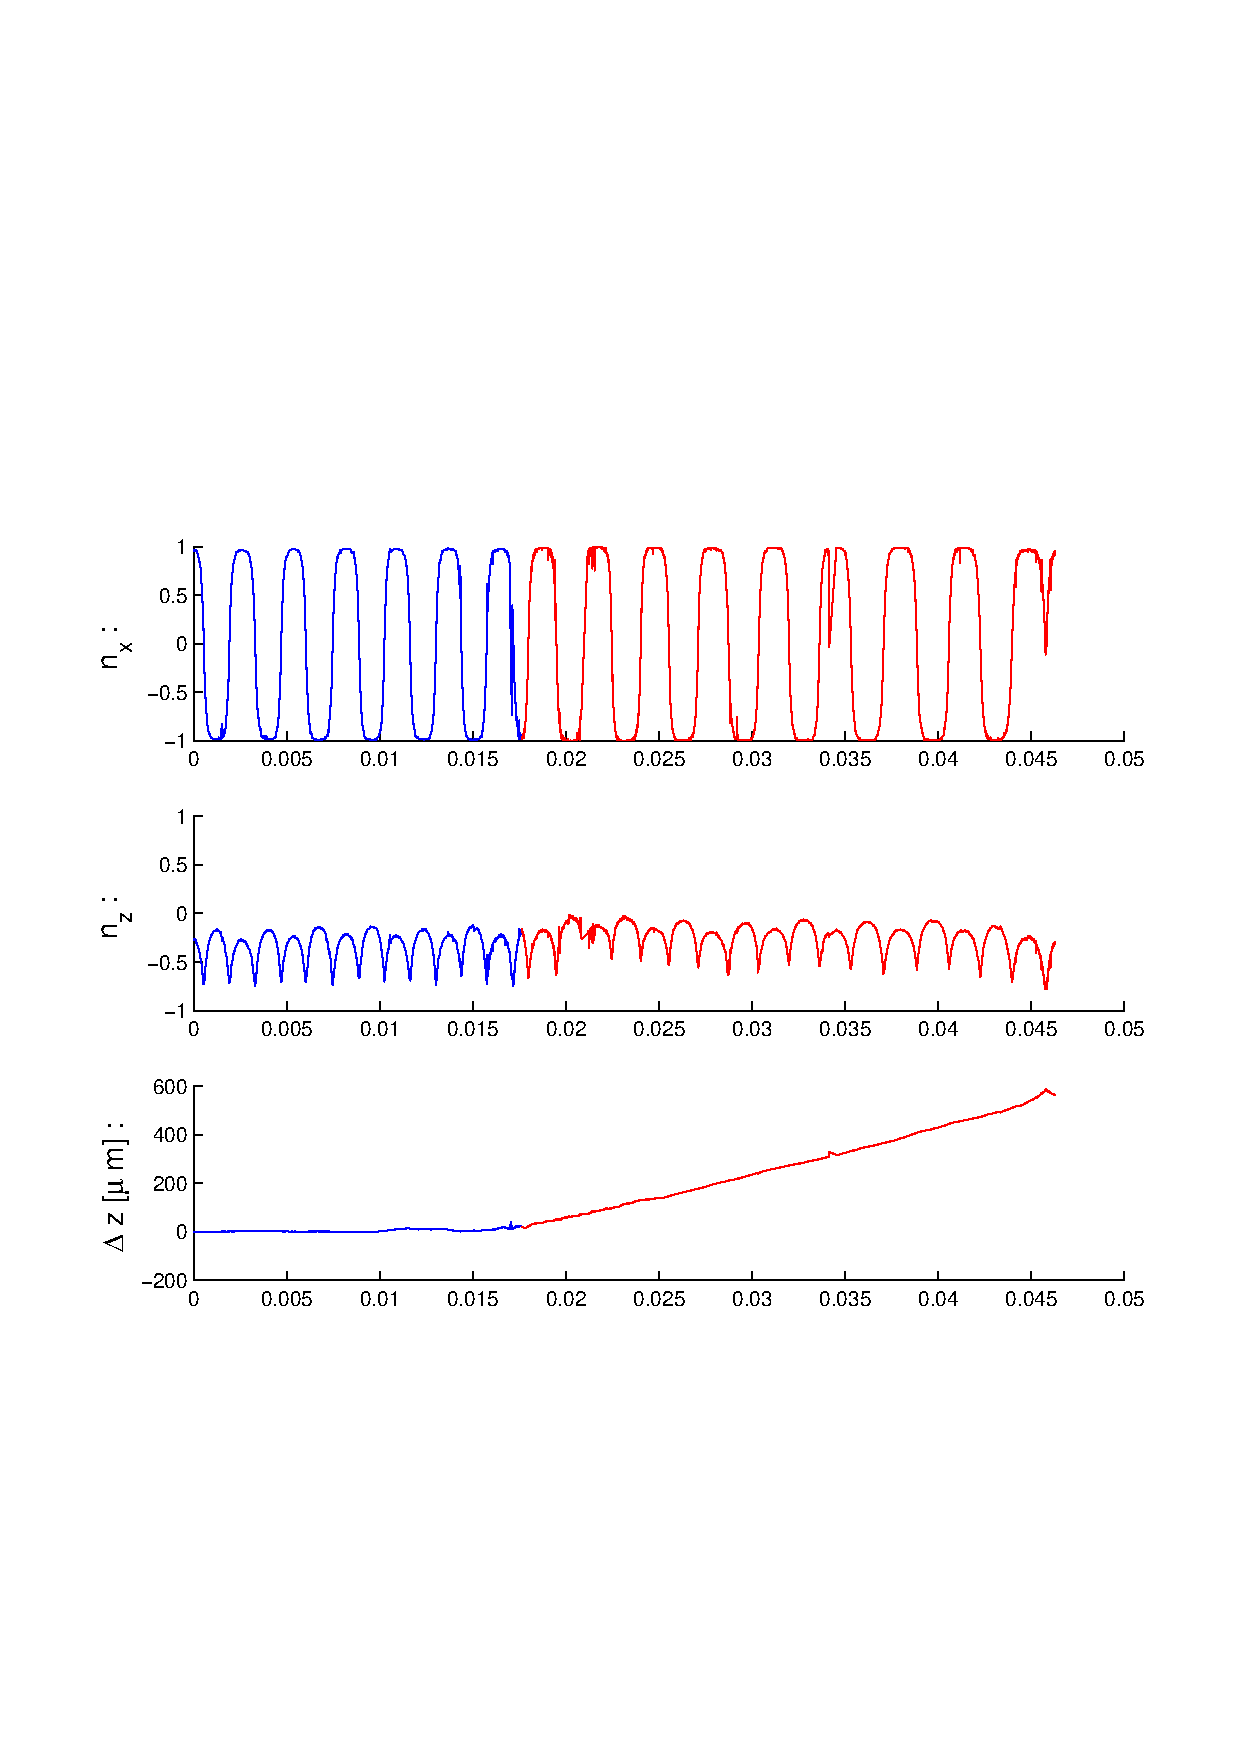
\includegraphics[width=0.8\textwidth]{Images/Particle 23/Particle23.pdf}
\caption{Particle 23: $ \lambda: 5.6106$Depth: 80 out of $200 \mu $ m}
\end{figure}

\begin{figure}[H]
\centering
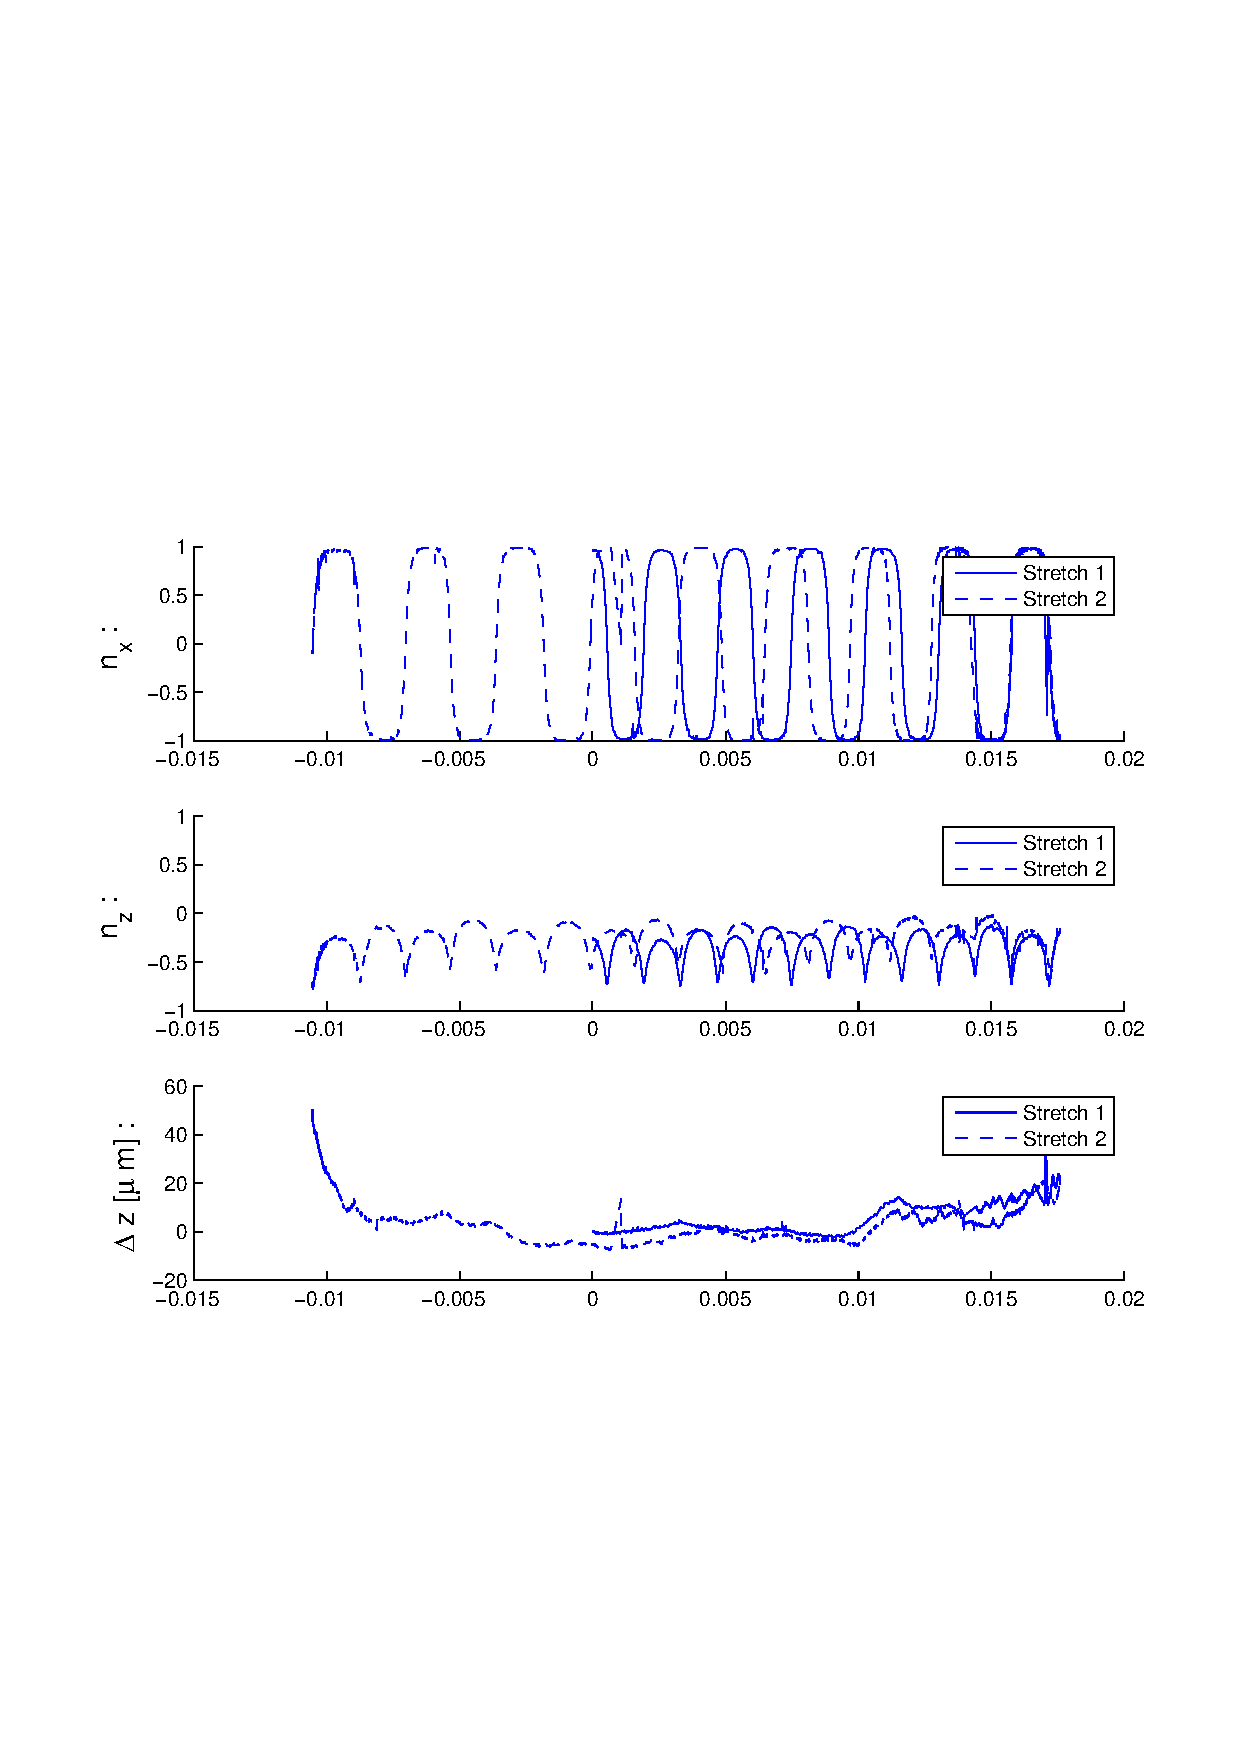
\includegraphics[width=0.8\textwidth]{Images/Particle 23/Stretch1.pdf}
\end{figure}




%
%\section{$\mathbf{\lambda}$ of about 6}
%These are the particles with a $\lambda = 7 \pm 0.5$
%\subsection{Particle 2}

\begin{figure}[ H]

\caption{Particle 2: $ \lambda: 13.9227$Depth: 30 out of $200 \mu $ m}

\centering

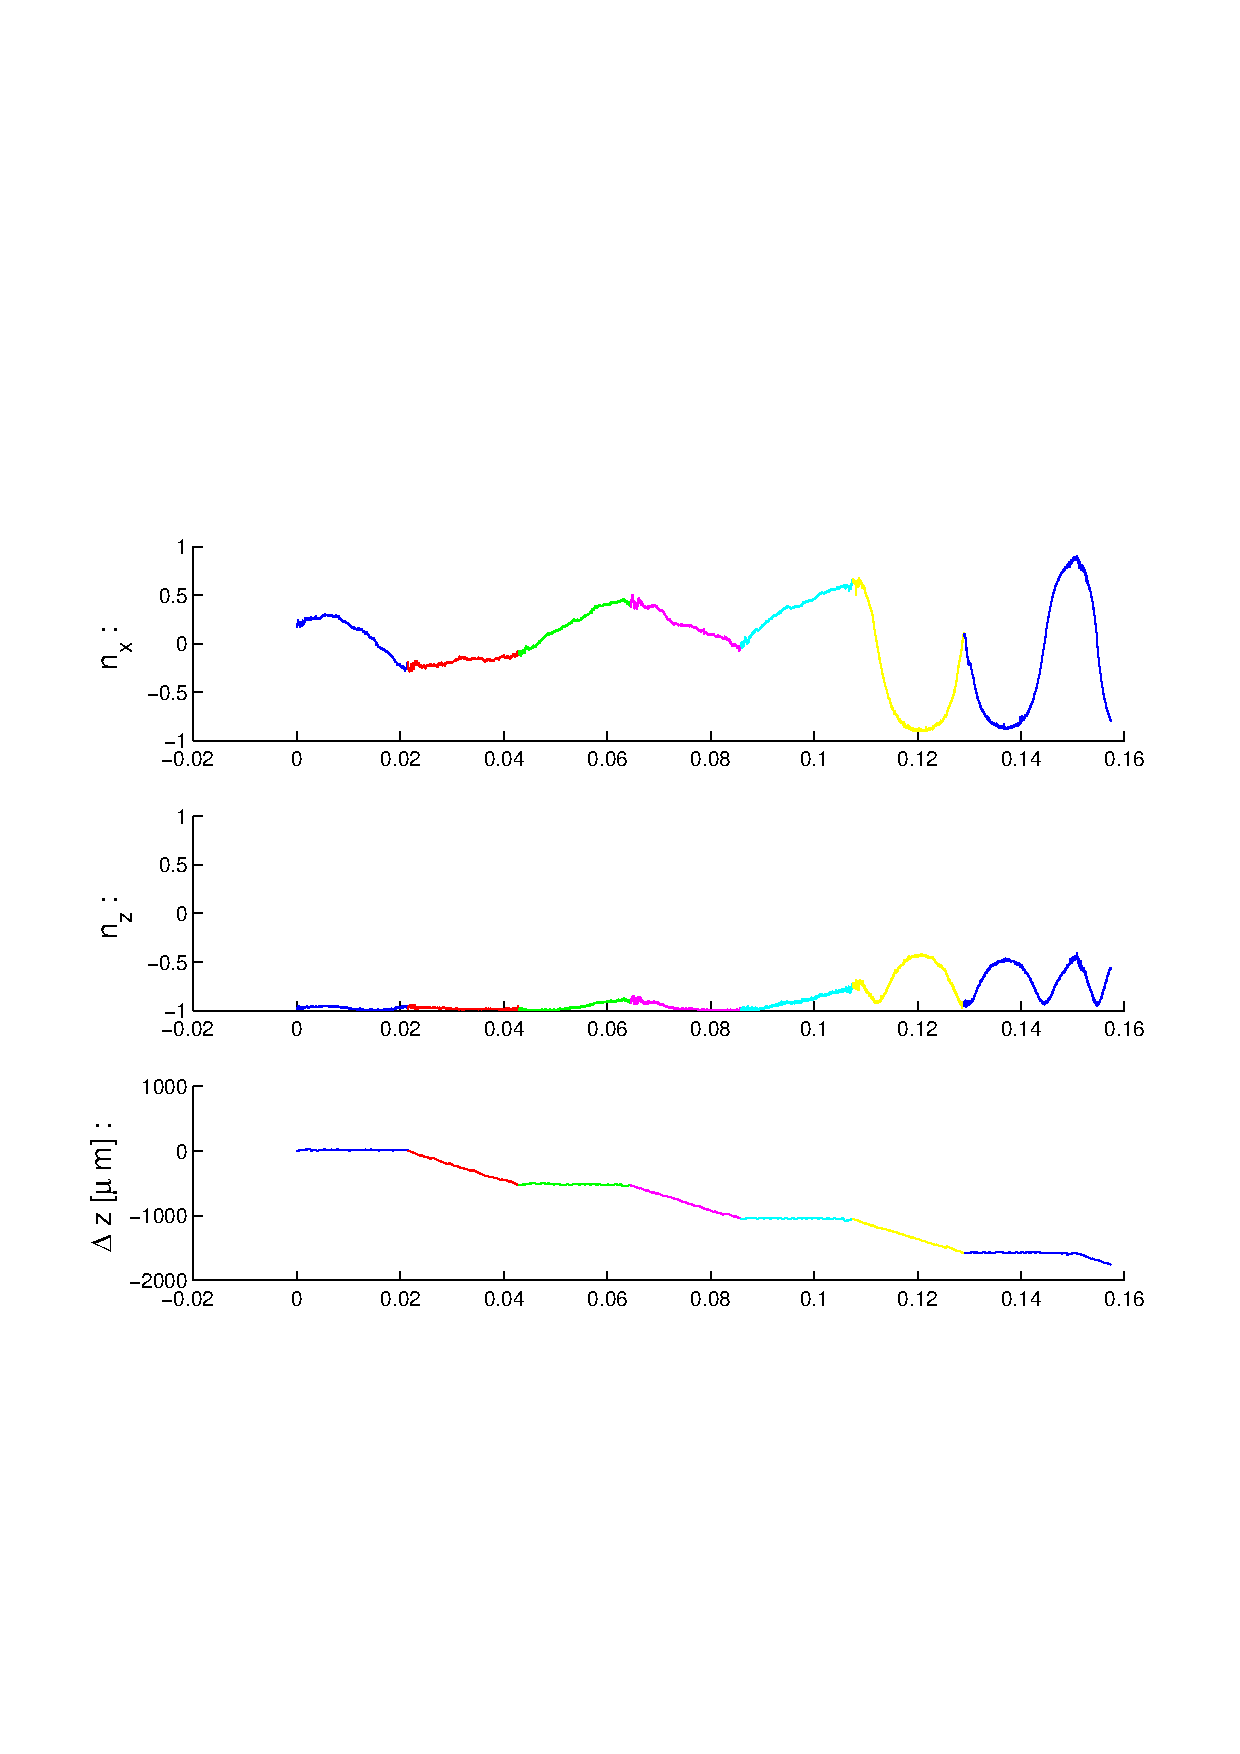
\includegraphics[width=0.8\textwidth]{Images/Particle 2/Particle2.pdf}

\end{figure}

\begin{figure}[ H]

\centering

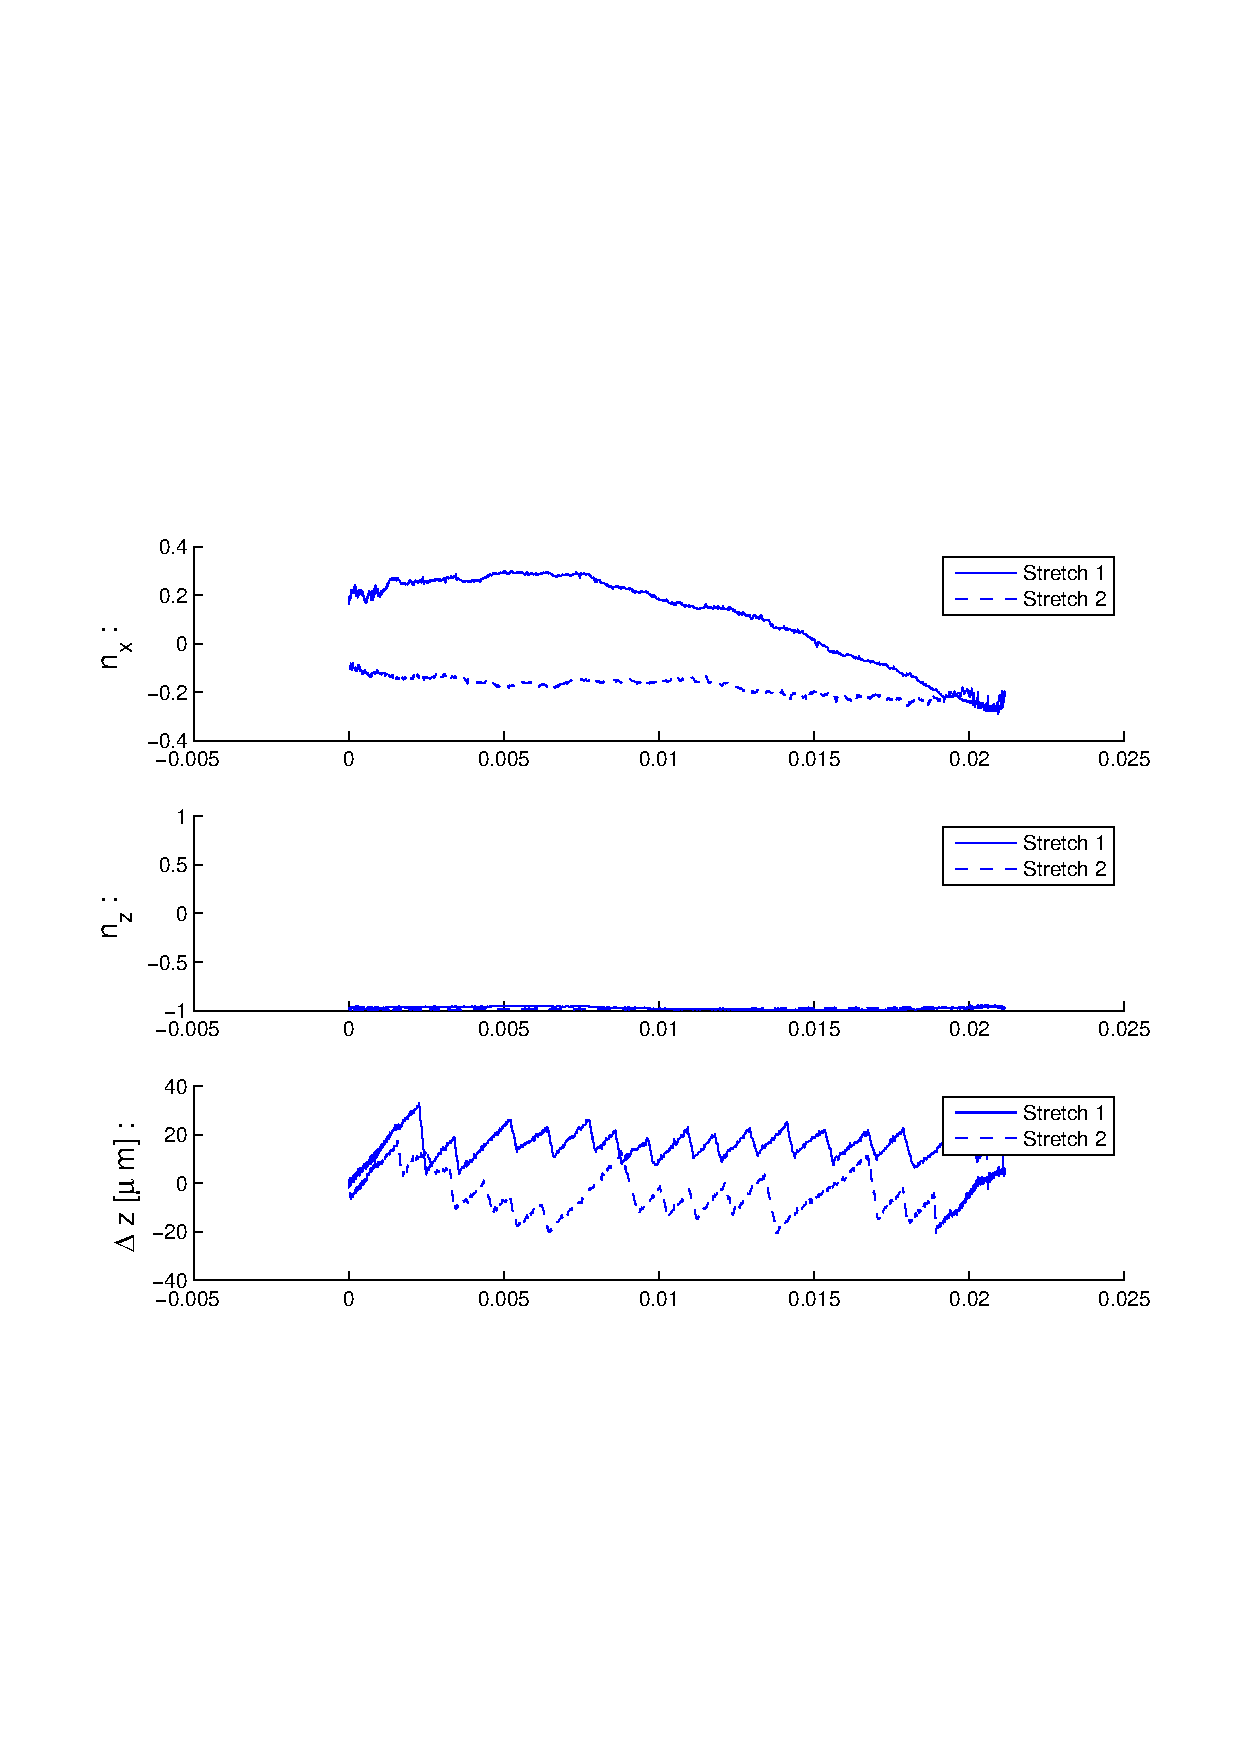
\includegraphics[width=0.8\textwidth]{Images/Particle 2/Stretch1.pdf}

\end{figure}

\begin{figure}[ H]

\centering

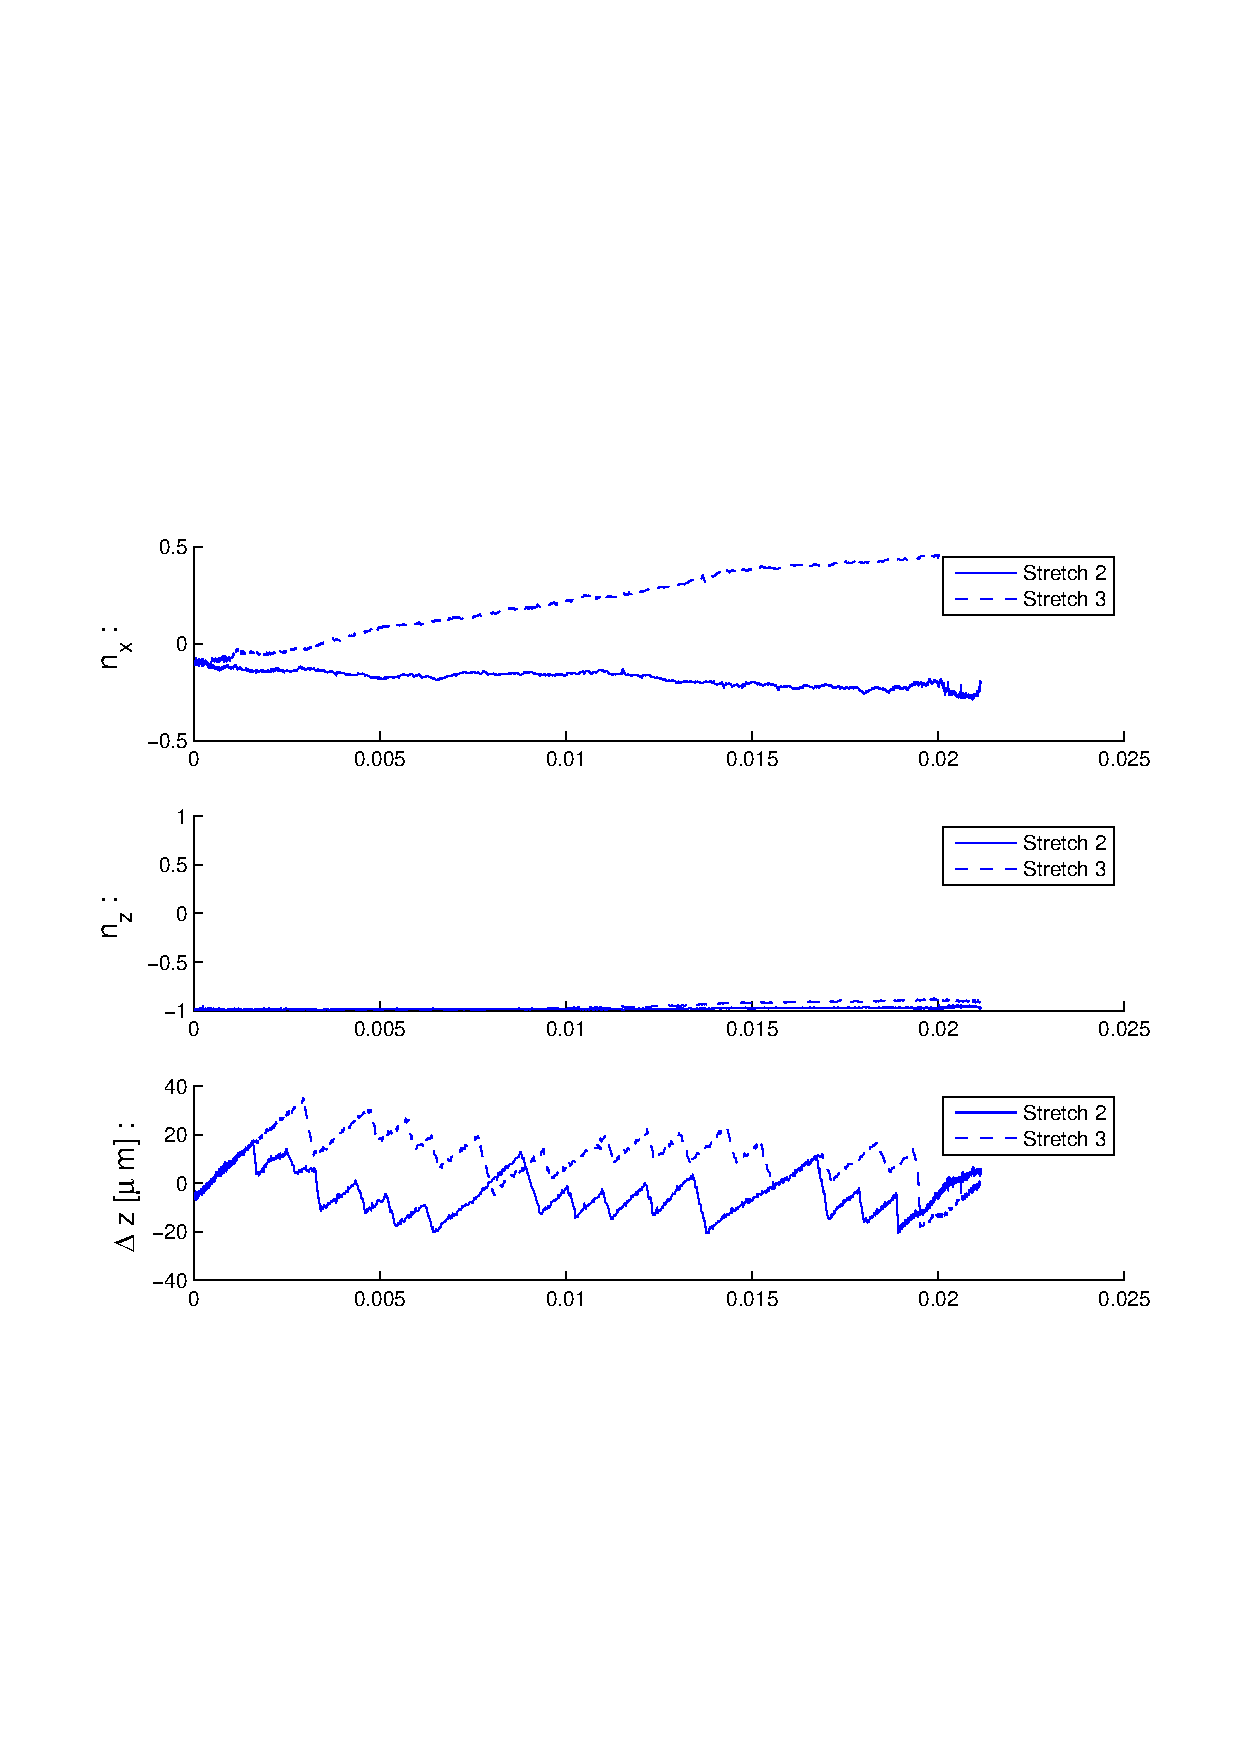
\includegraphics[width=0.8\textwidth]{Images/Particle 2/Stretch2.pdf}

\end{figure}

\begin{figure}[ H]

\centering

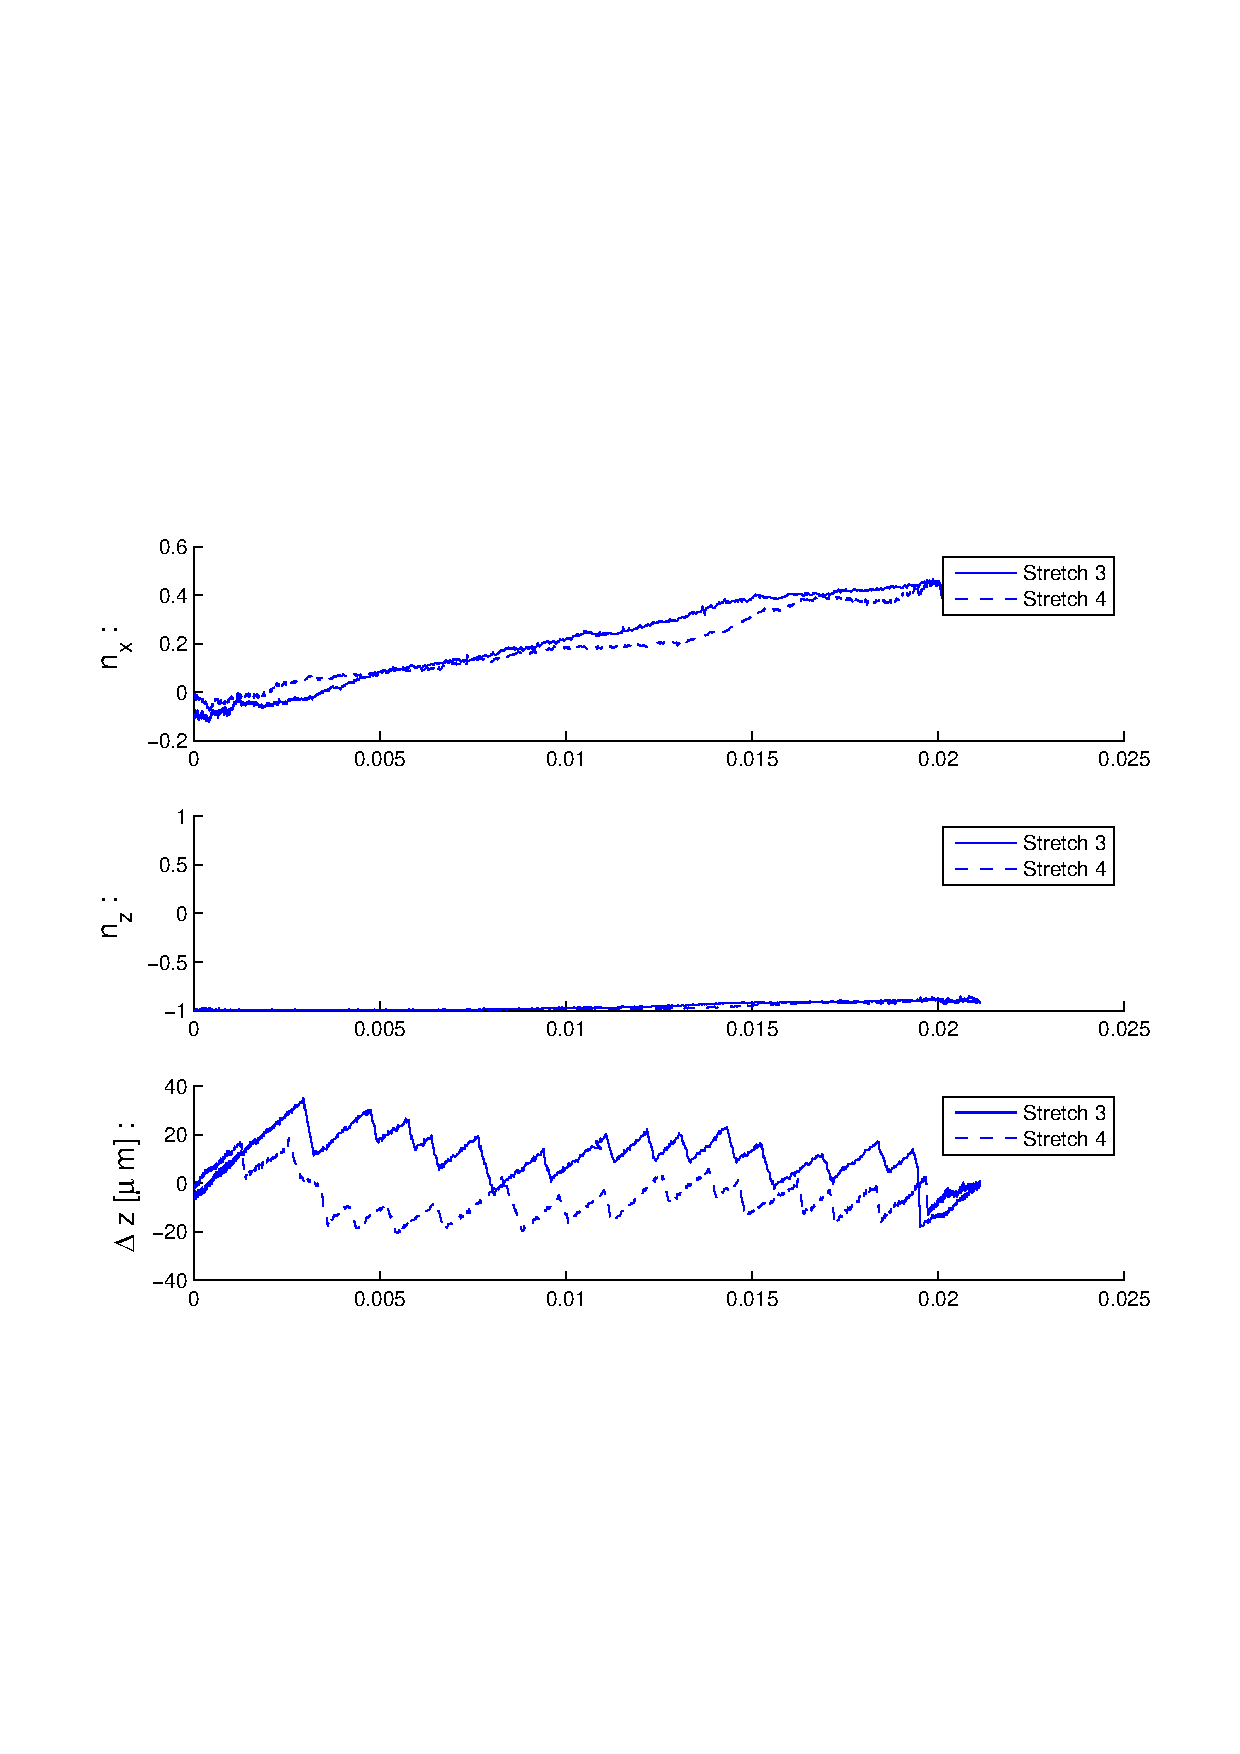
\includegraphics[width=0.8\textwidth]{Images/Particle 2/Stretch3.pdf}

\end{figure}

\begin{figure}[ H]

\centering

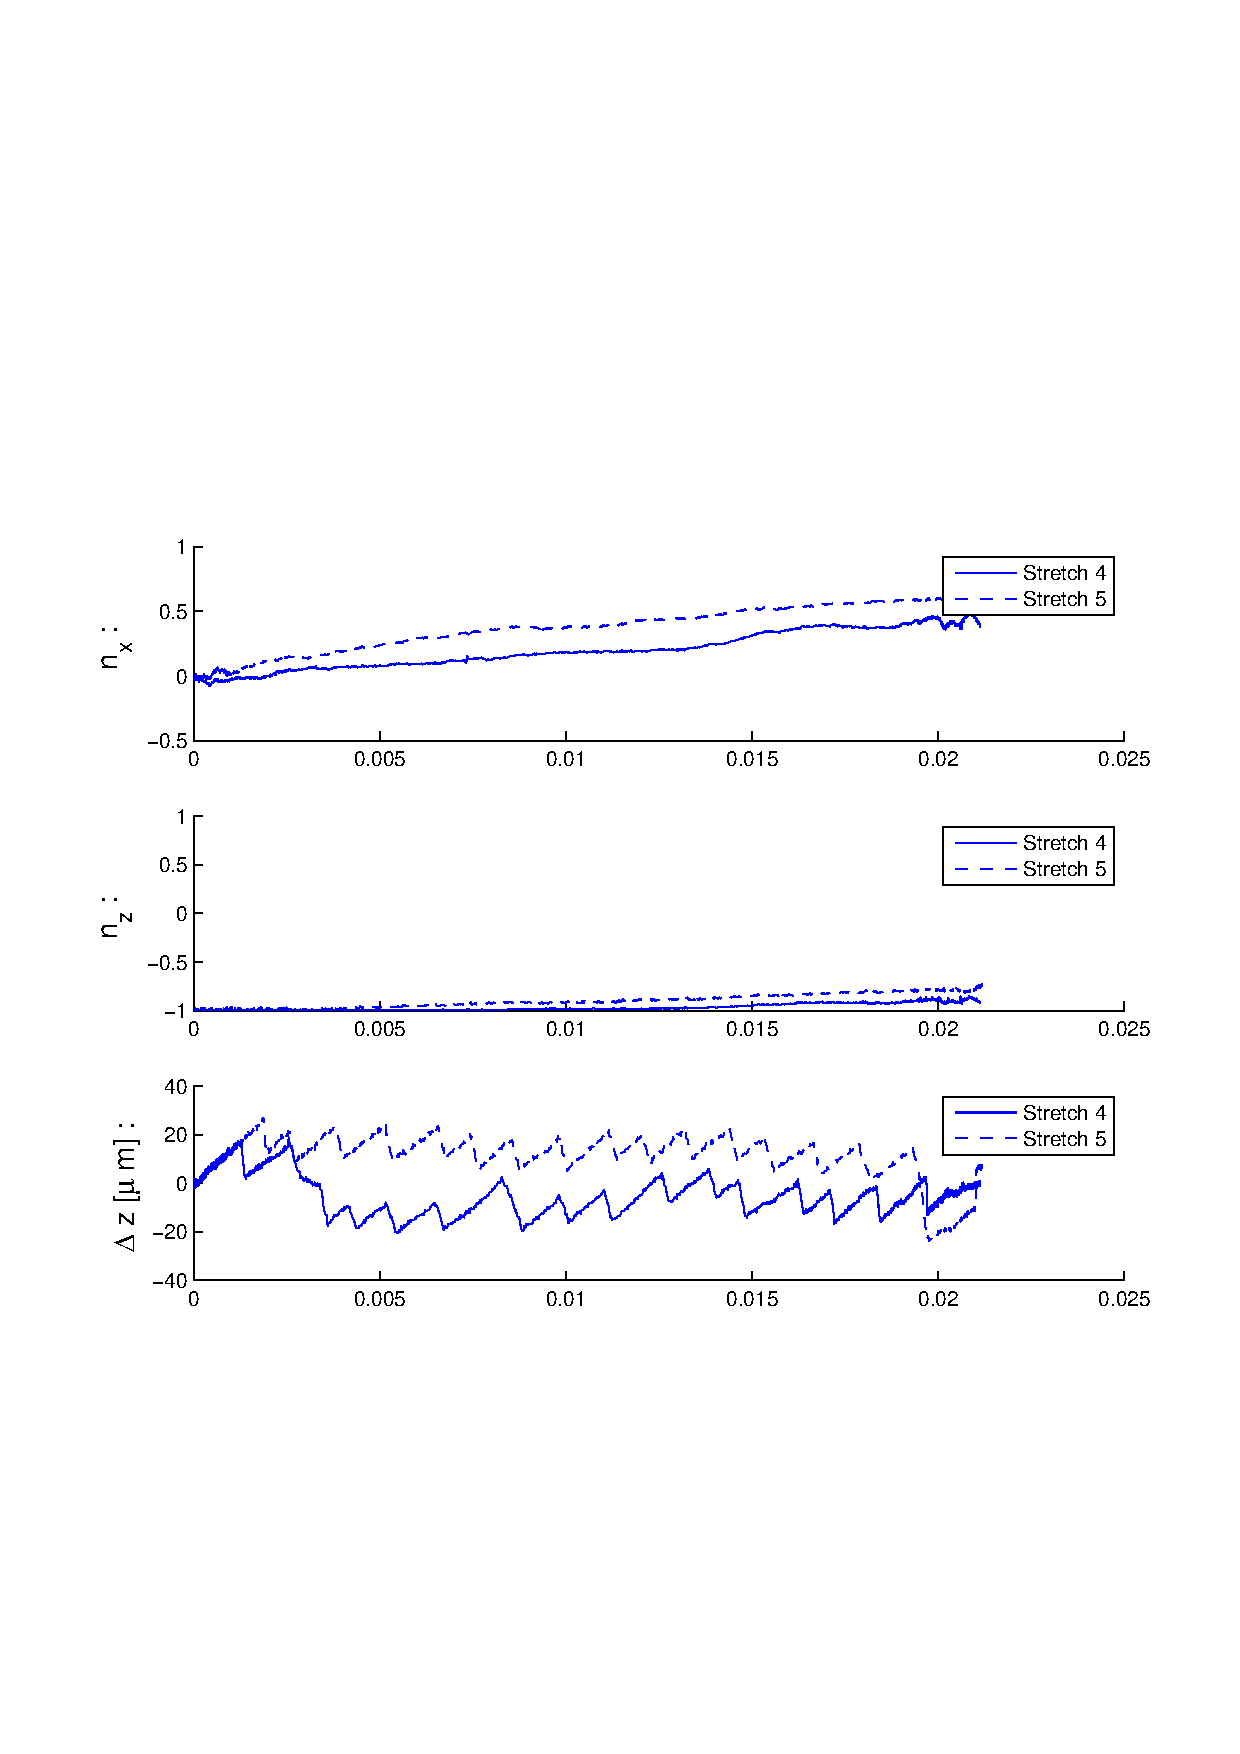
\includegraphics[width=0.8\textwidth]{Images/Particle 2/Stretch4.pdf}

\end{figure}

\begin{figure}[ H]

\centering

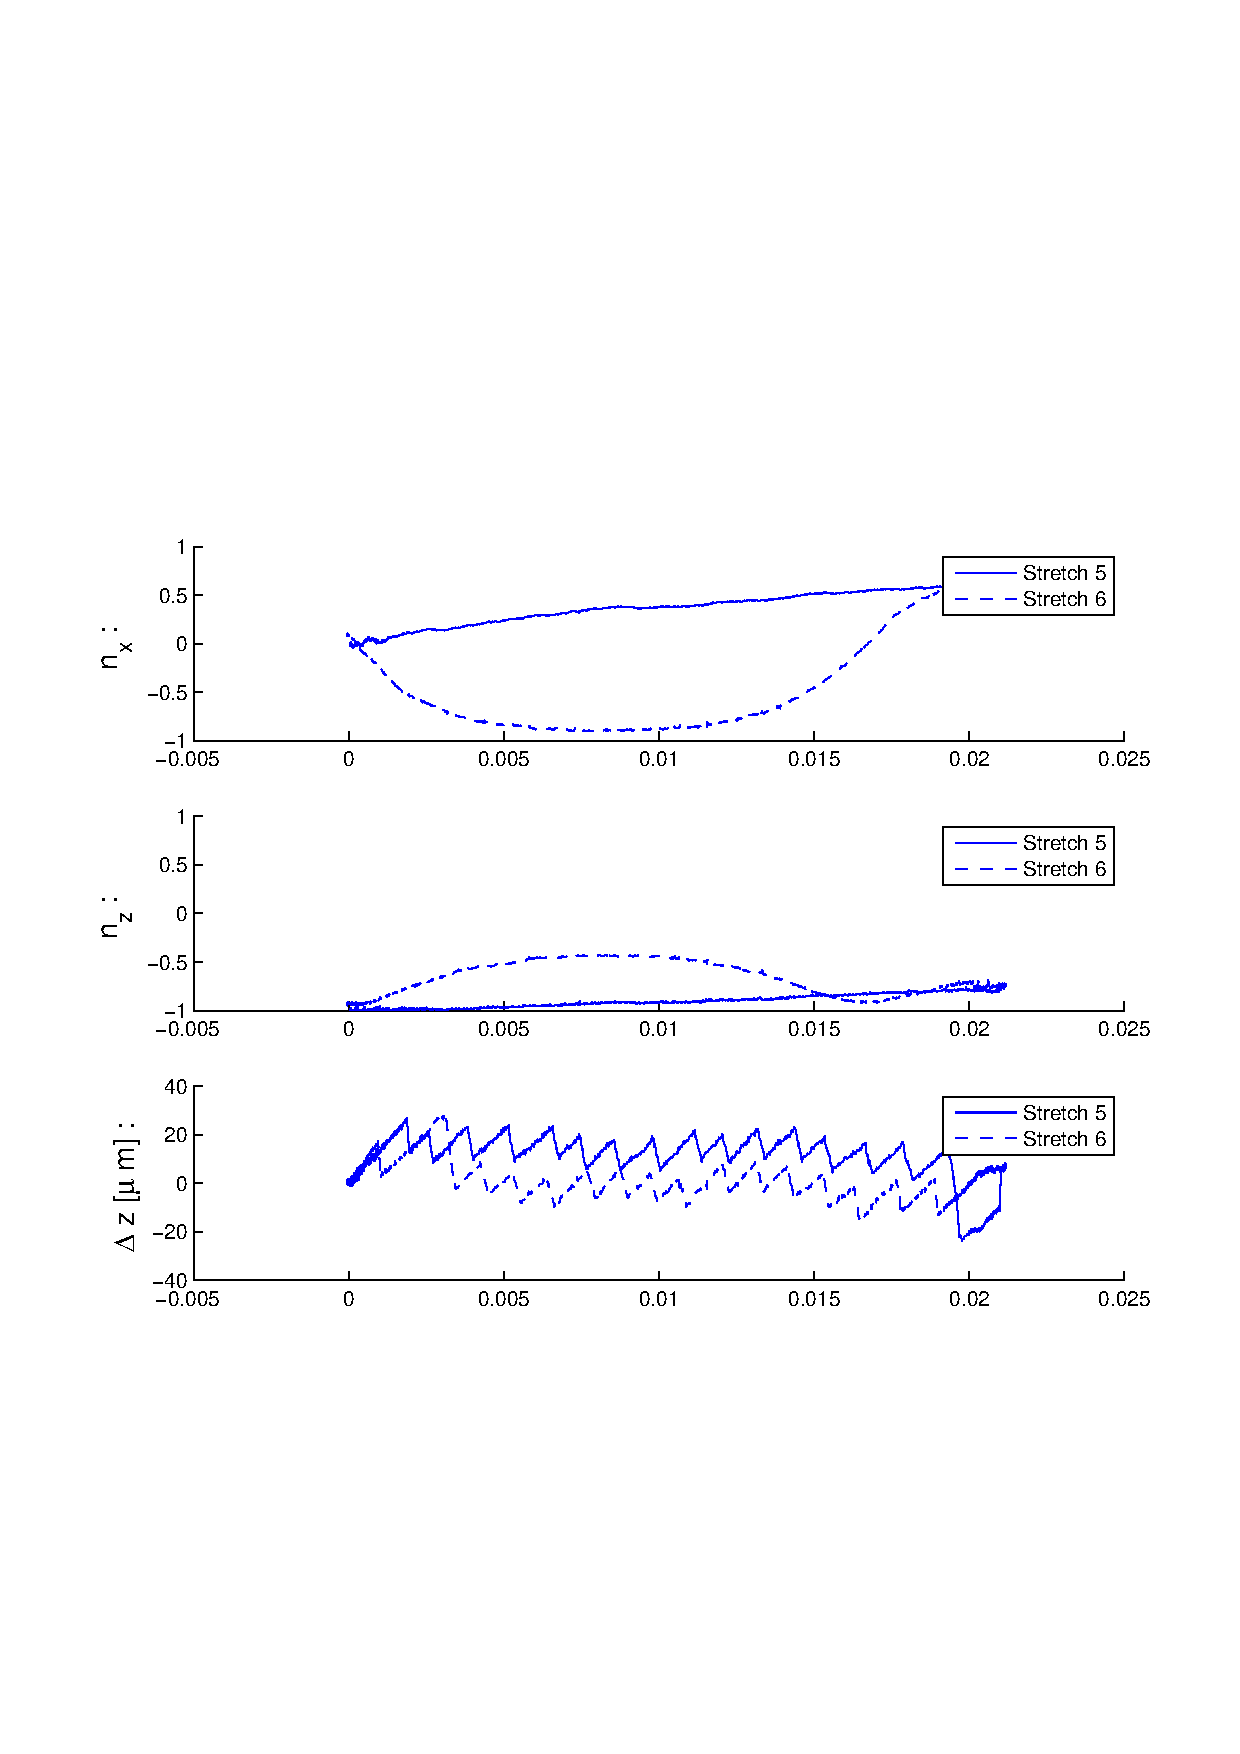
\includegraphics[width=0.8\textwidth]{Images/Particle 2/Stretch5.pdf}

\end{figure}

\begin{figure}[ H]

\centering

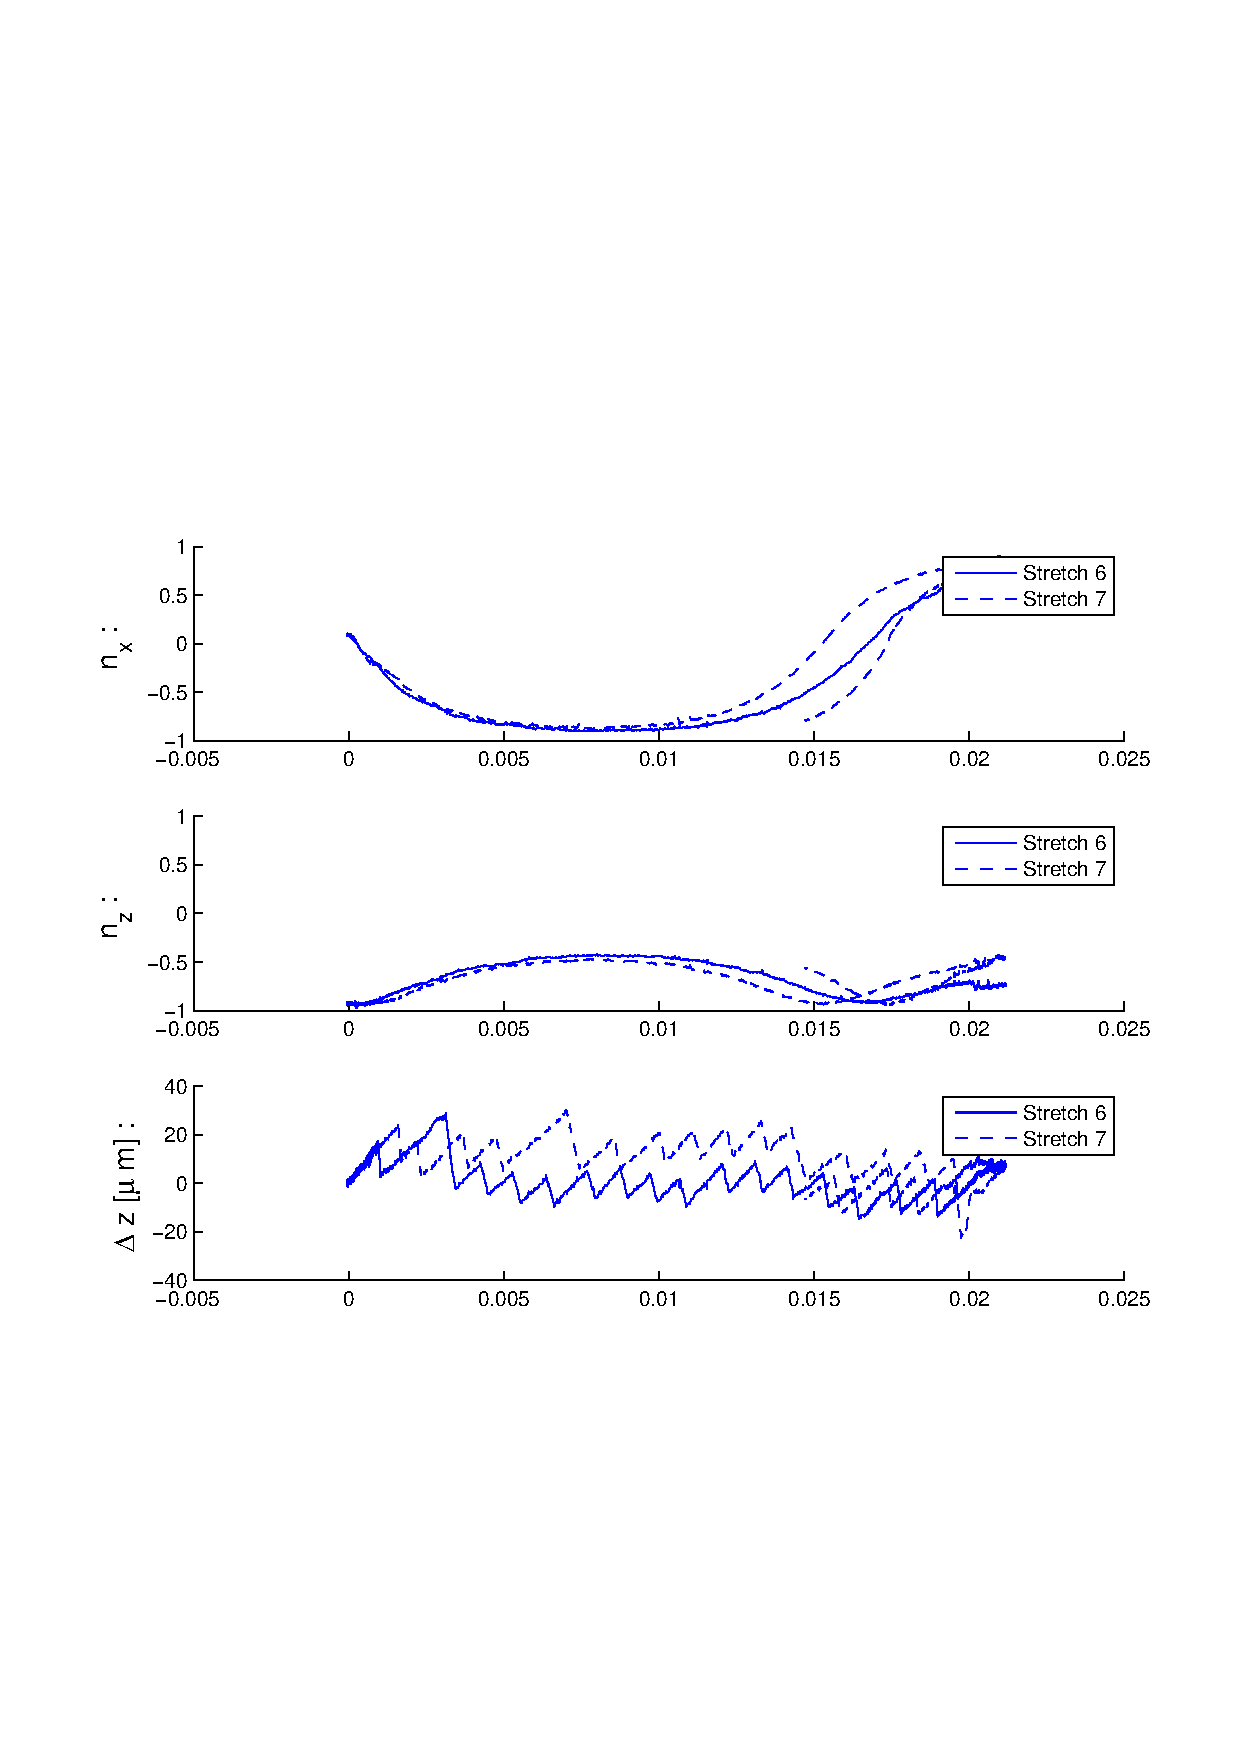
\includegraphics[width=0.8\textwidth]{Images/Particle 2/Stretch6.pdf}

\end{figure}


\subsection{Particle 7}

\begin{figure}[ H]

\caption{Particle 7: $ \lambda: 27.4694$Depth: 20 out of $200 \mu $ m}

\centering

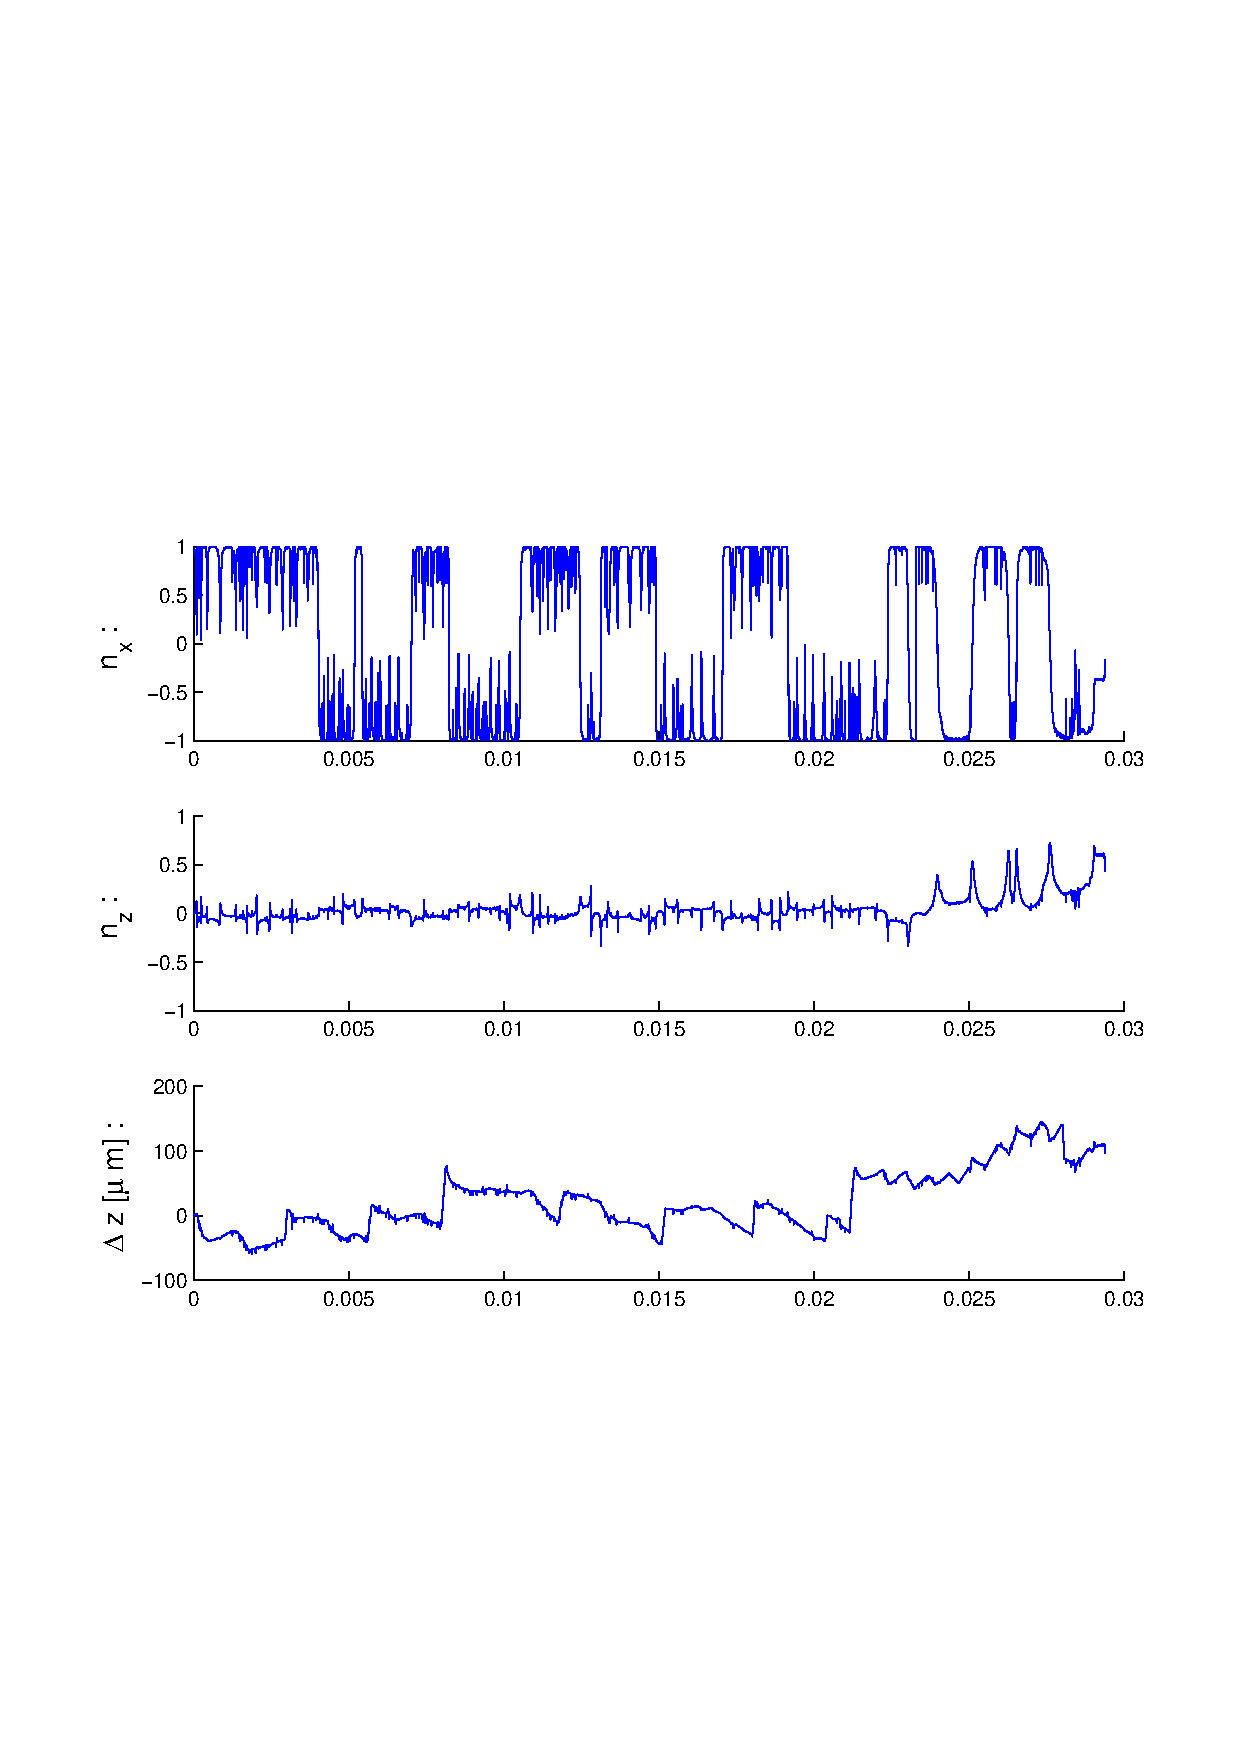
\includegraphics[width=0.8\textwidth]{Images/Particle 7/Particle7.pdf}

\end{figure}


\subsection{Particle 18}

\begin{figure}[ H]

\caption{Particle 18: Unclear. There are several possible interactions around 6 minutes but neither is all too clear. Also the second turn is overall quite jumpy$ \lambda: 14.3568$Depth: 20 out of $200 \mu $ m}

\centering

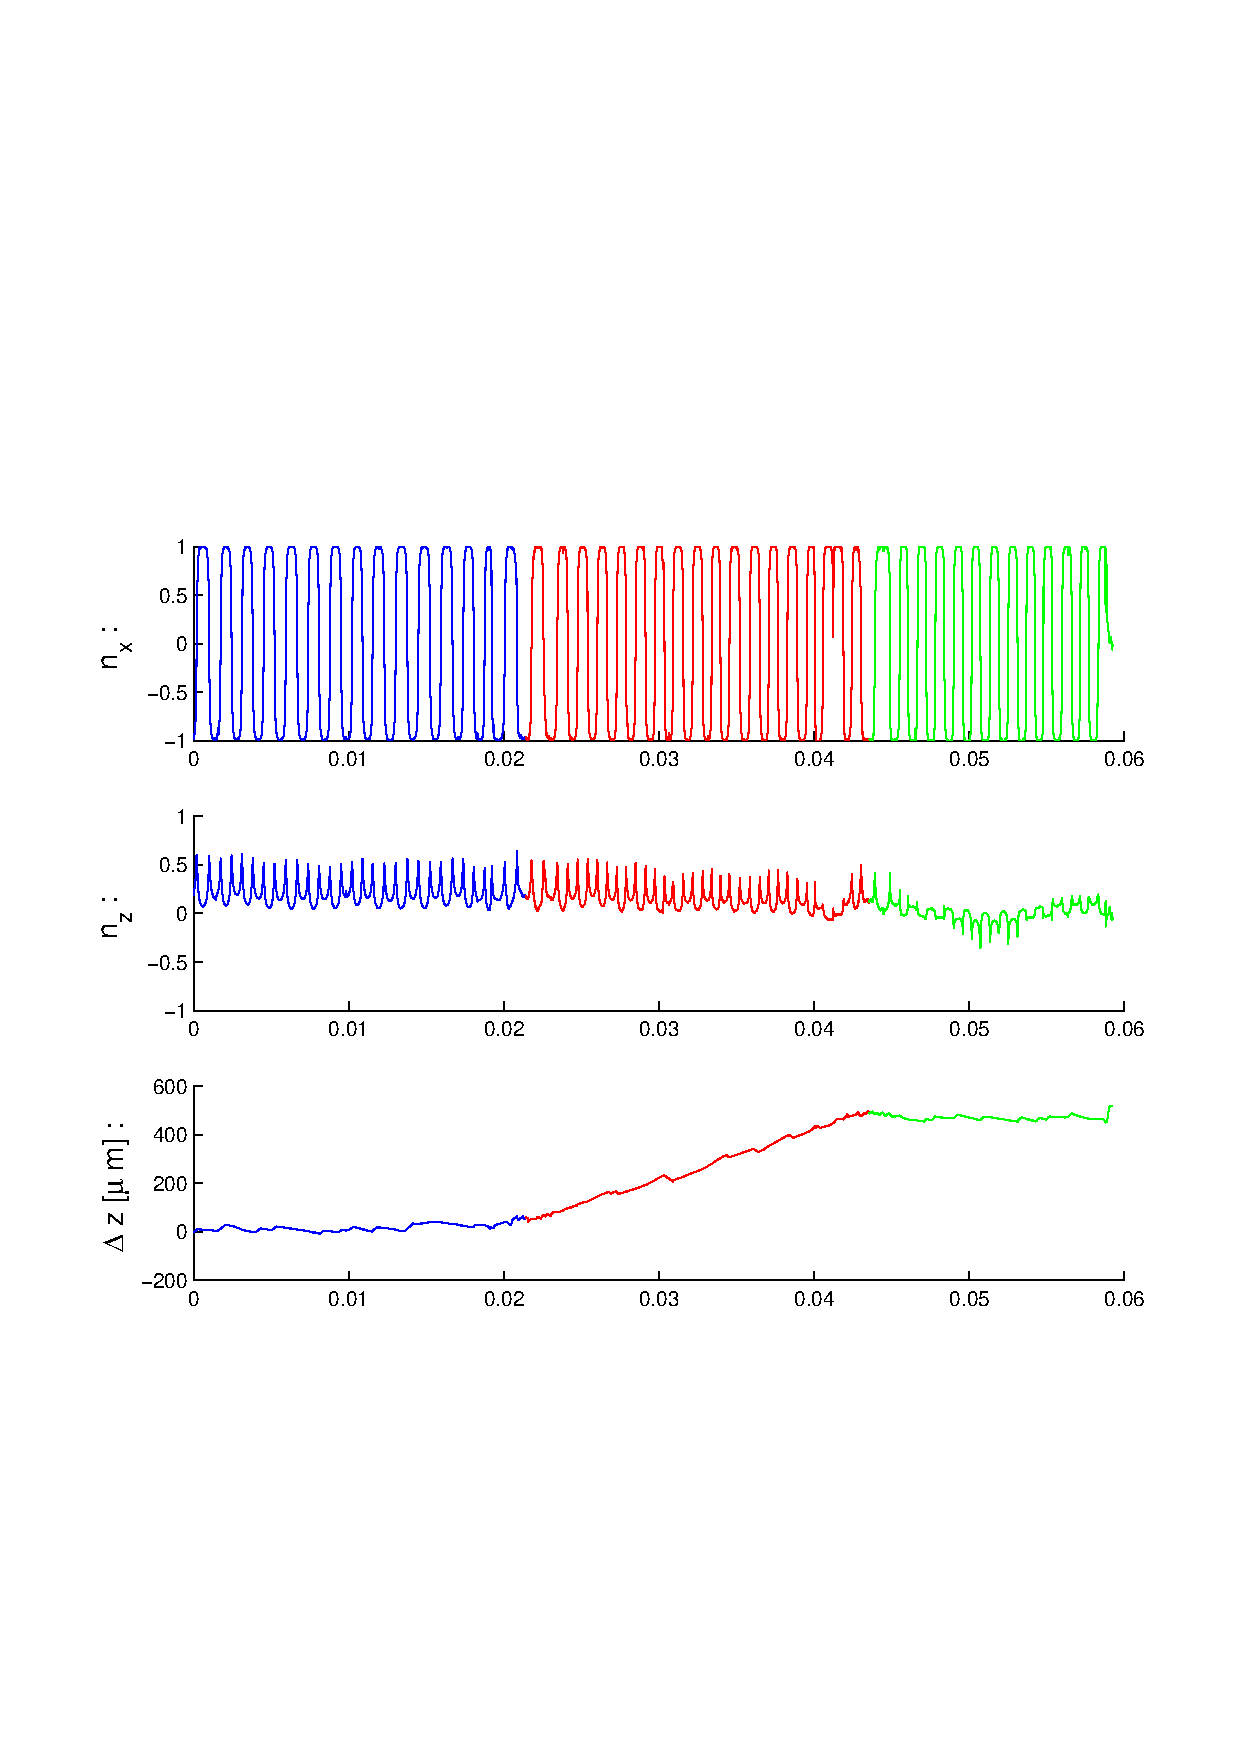
\includegraphics[width=0.8\textwidth]{Images/Particle 18/Particle18.pdf}

\end{figure}

\begin{figure}[ H]

\centering

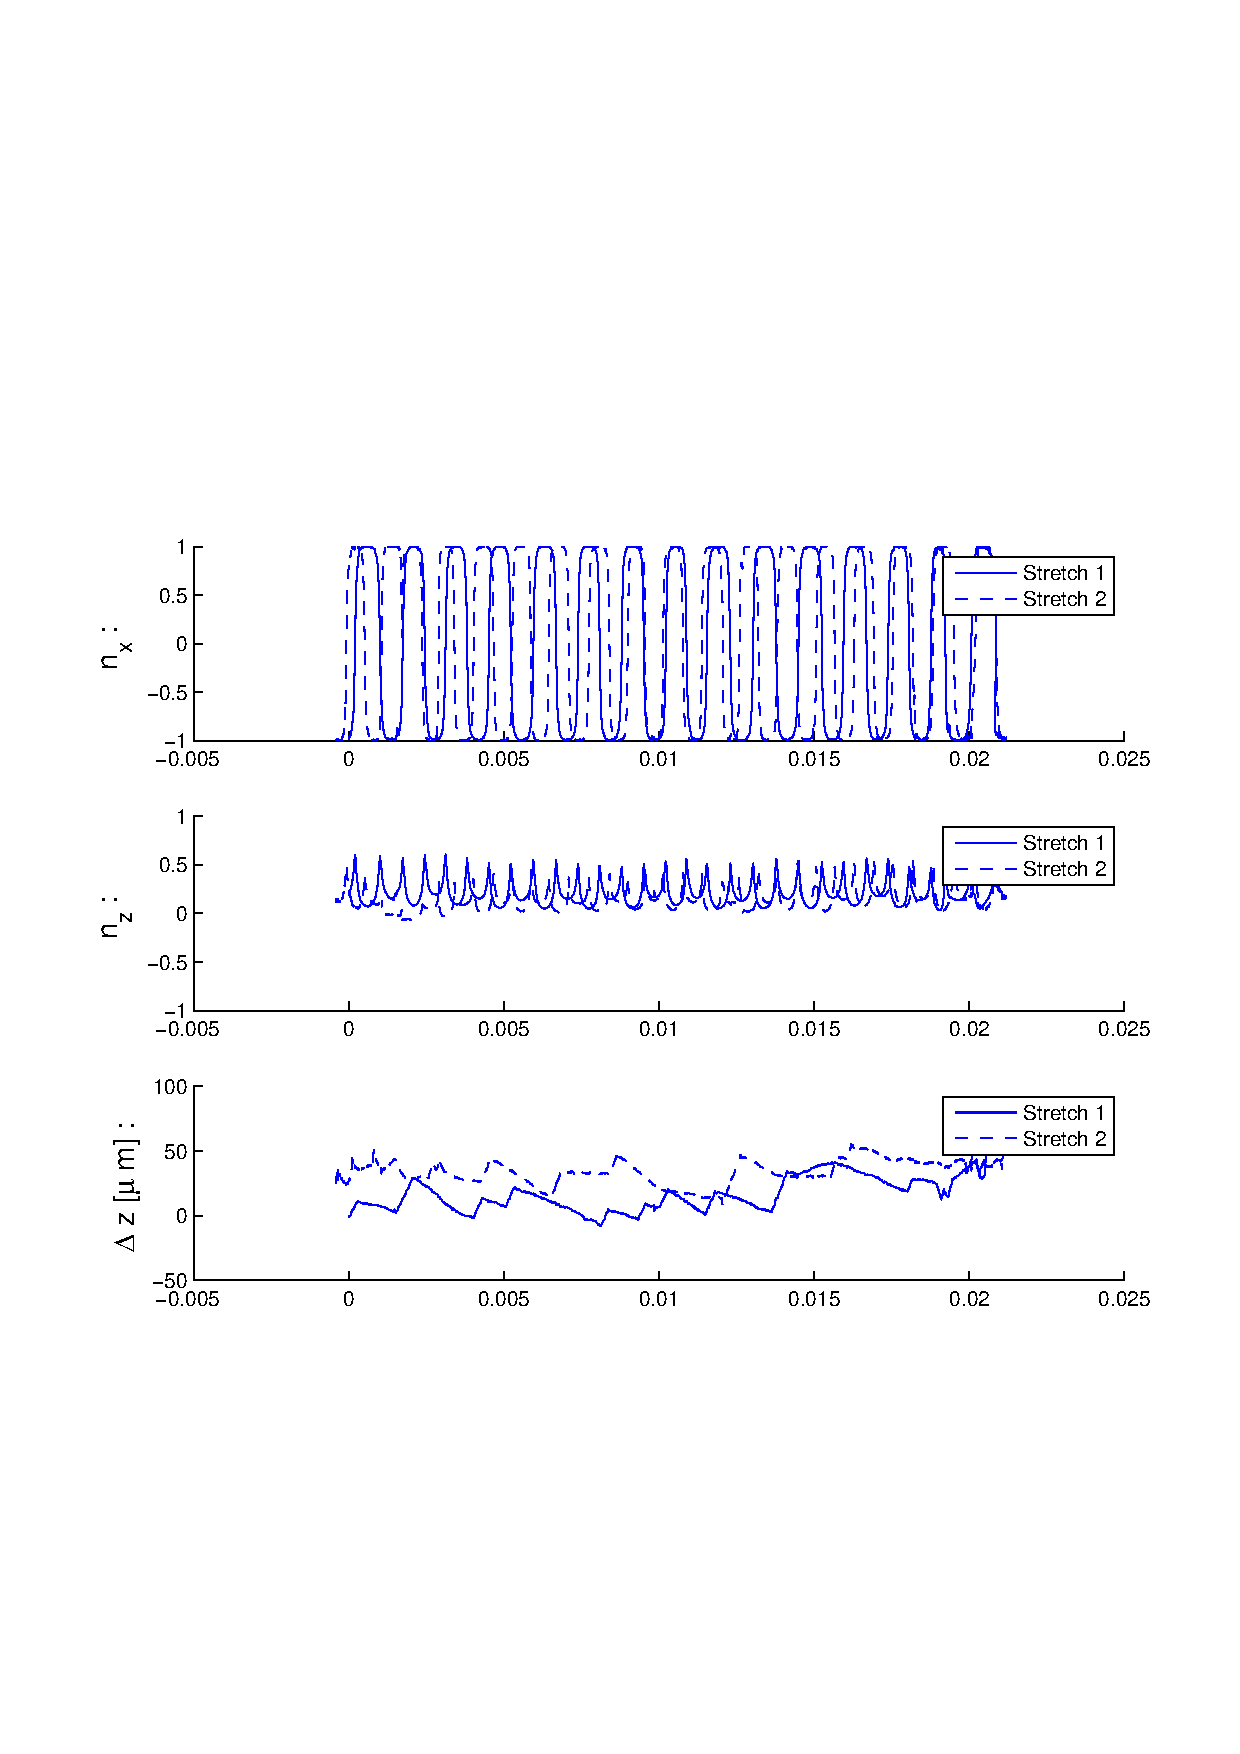
\includegraphics[width=0.8\textwidth]{Images/Particle 18/Stretch1.pdf}

\end{figure}

\begin{figure}[ H]

\centering

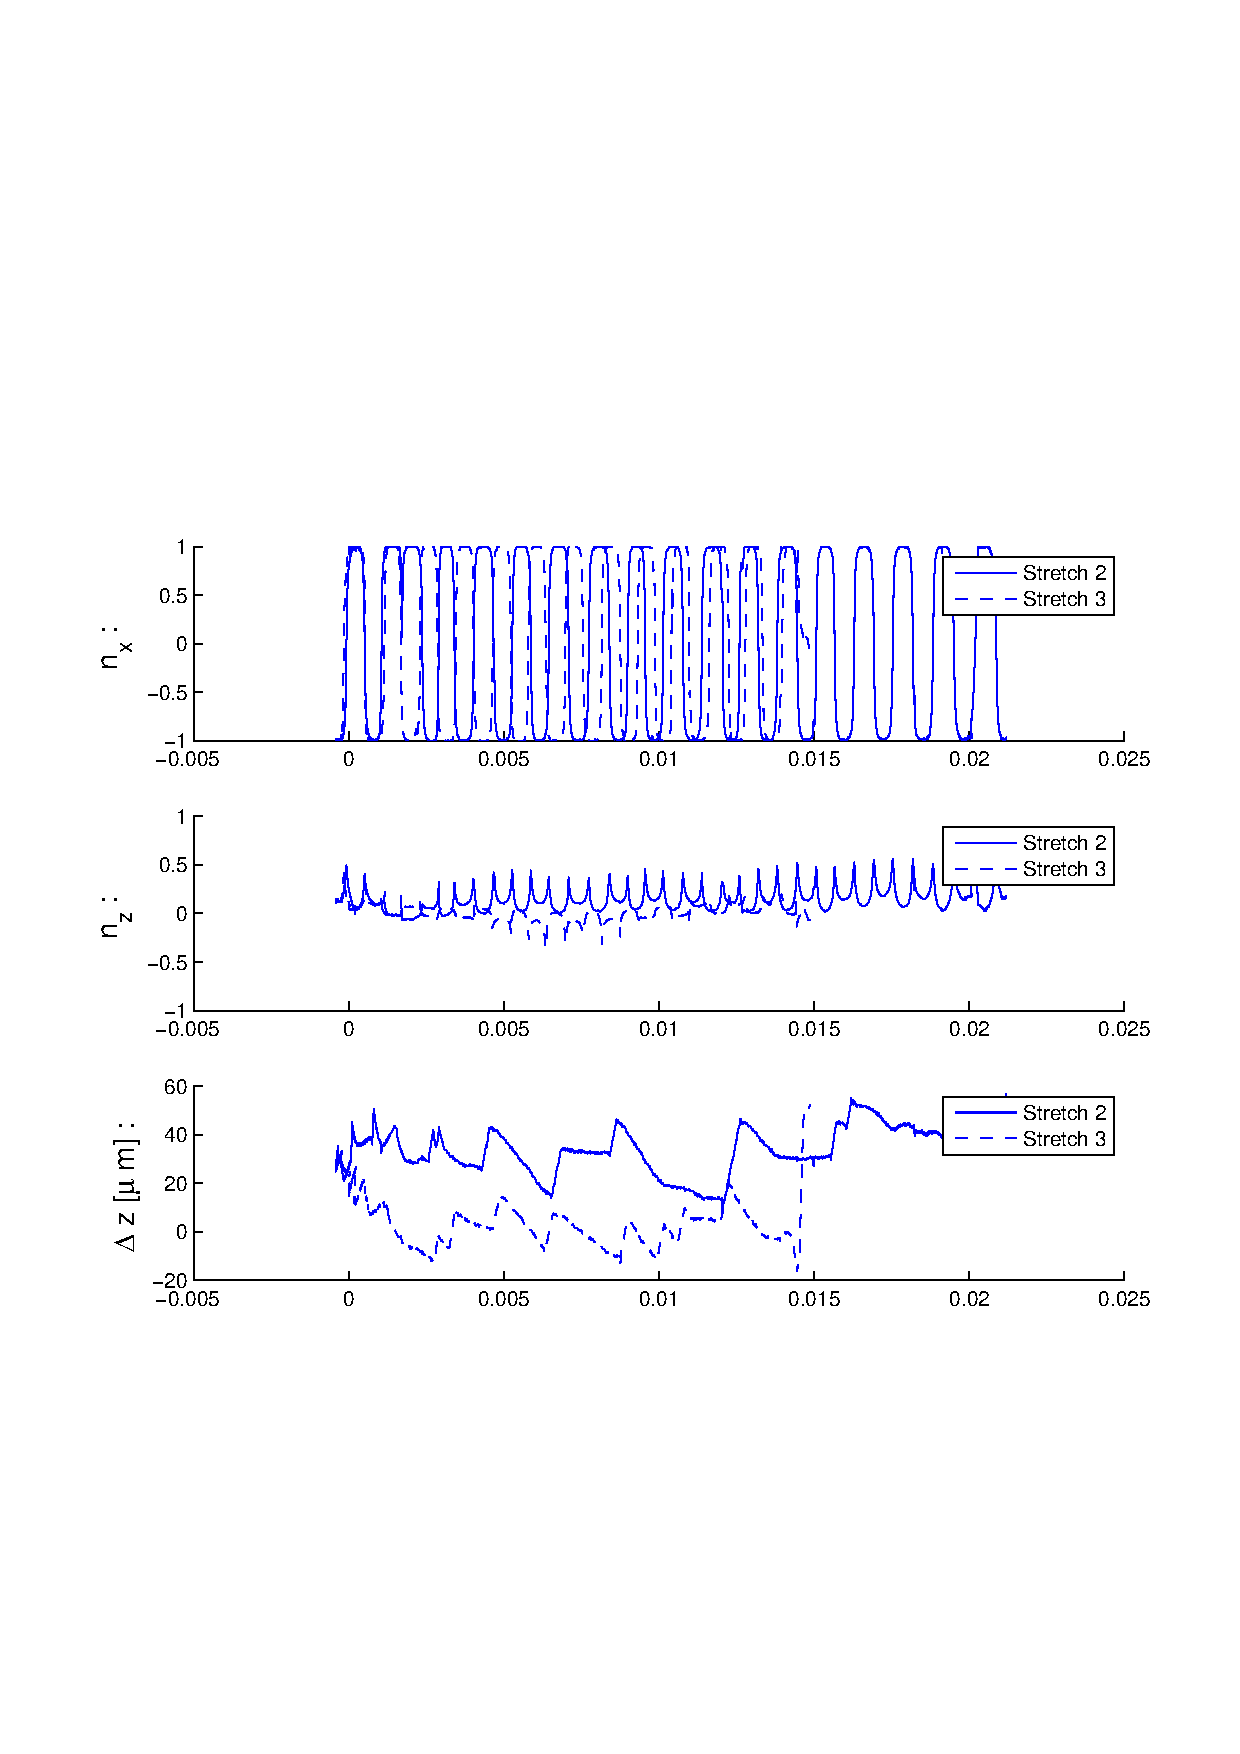
\includegraphics[width=0.8\textwidth]{Images/Particle 18/Stretch2.pdf}

\end{figure}


\subsection{Particle 19}

\begin{figure}[ H]

\caption{Particle 19: At around 0:50 there is an uneven vertical flow "surging" the particle down. $ \lambda: 13.795$Depth: 120 out of $200 \mu $ m}

\centering

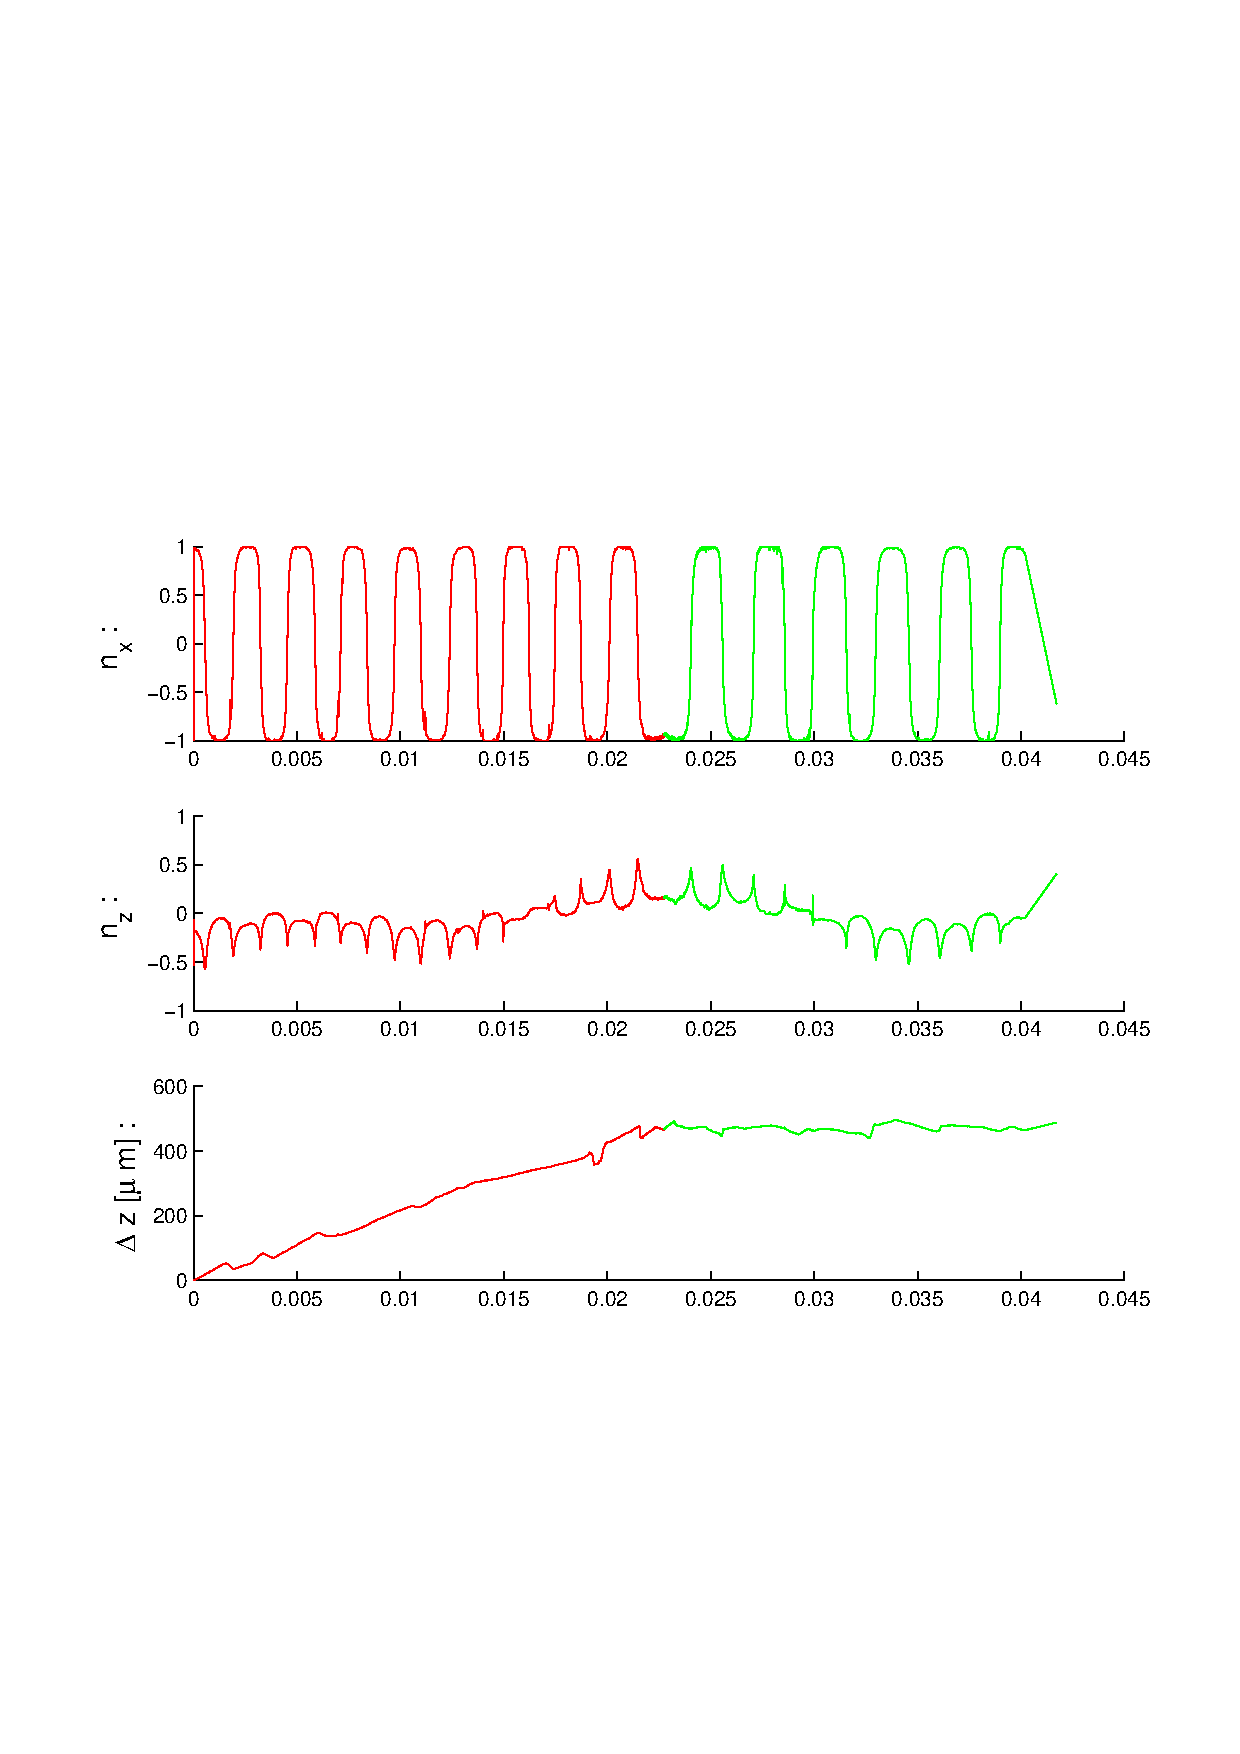
\includegraphics[width=0.8\textwidth]{Images/Particle 19/Particle19.pdf}

\end{figure}

\begin{figure}[ H]

\centering

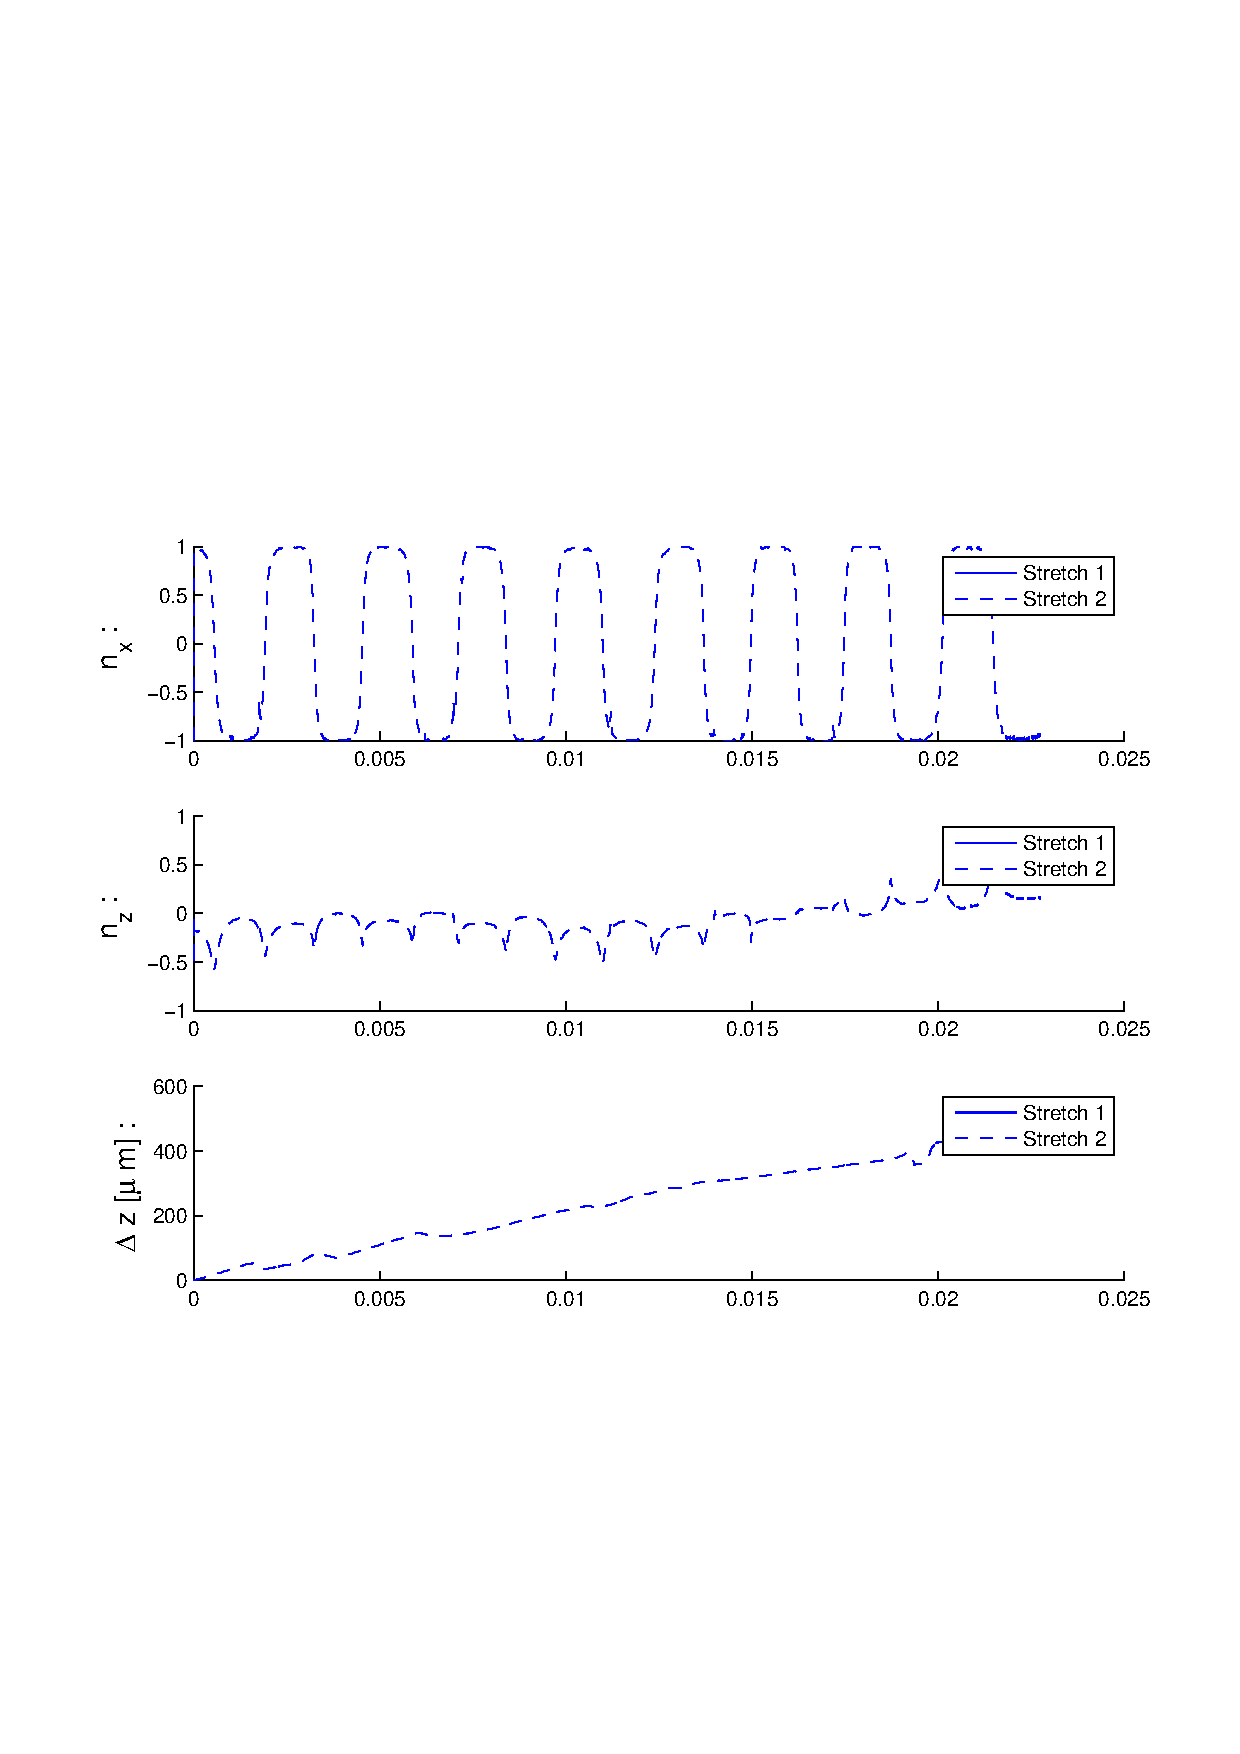
\includegraphics[width=0.8\textwidth]{Images/Particle 19/Stretch1.pdf}

\end{figure}

\begin{figure}[ H]

\centering

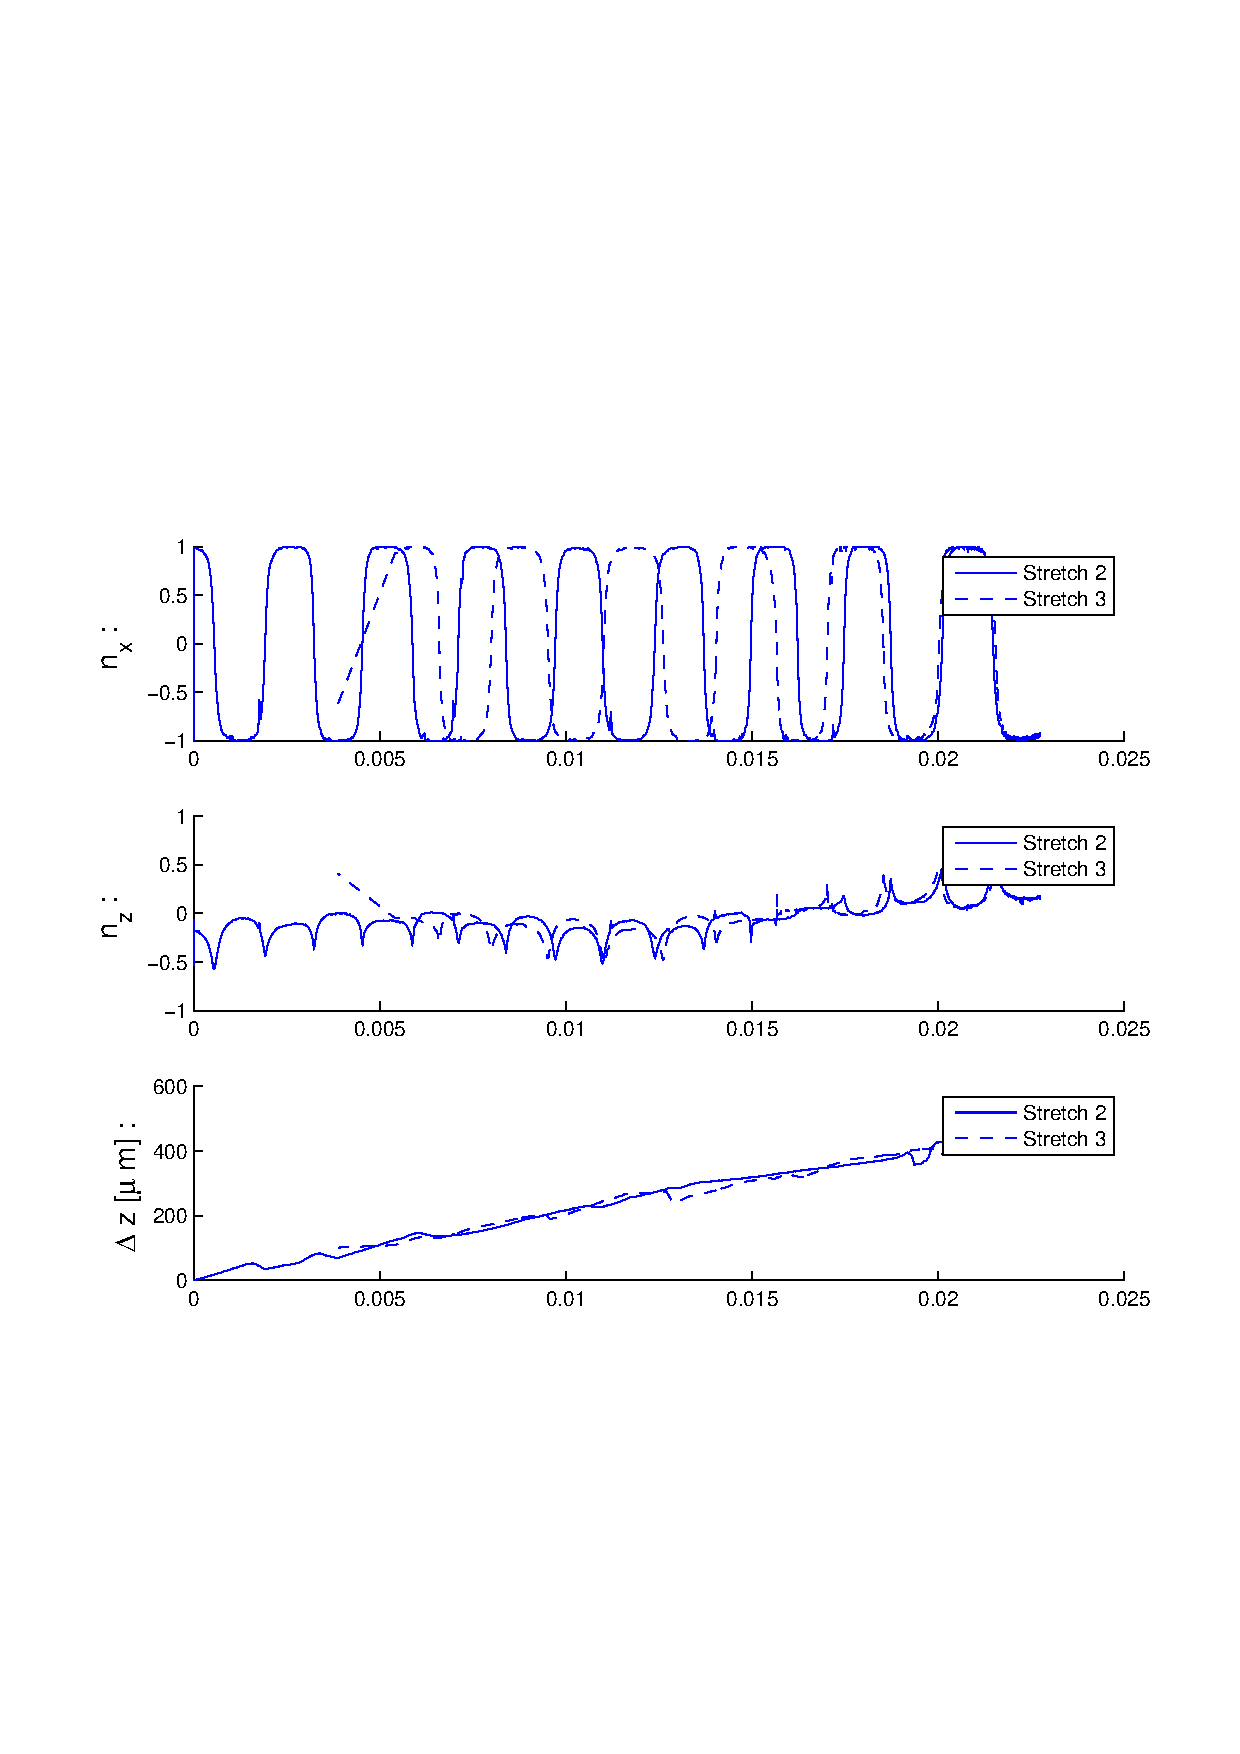
\includegraphics[width=0.8\textwidth]{Images/Particle 19/Stretch2.pdf}

\end{figure}



 


\subsection{Particle 20}

\begin{figure}[ H]

\caption{Particle 20: At 5:22 collides with large "debris" on channel floor. $ \lambda: 13.5864$Depth: 150 out of $200 \mu $ m}

\centering

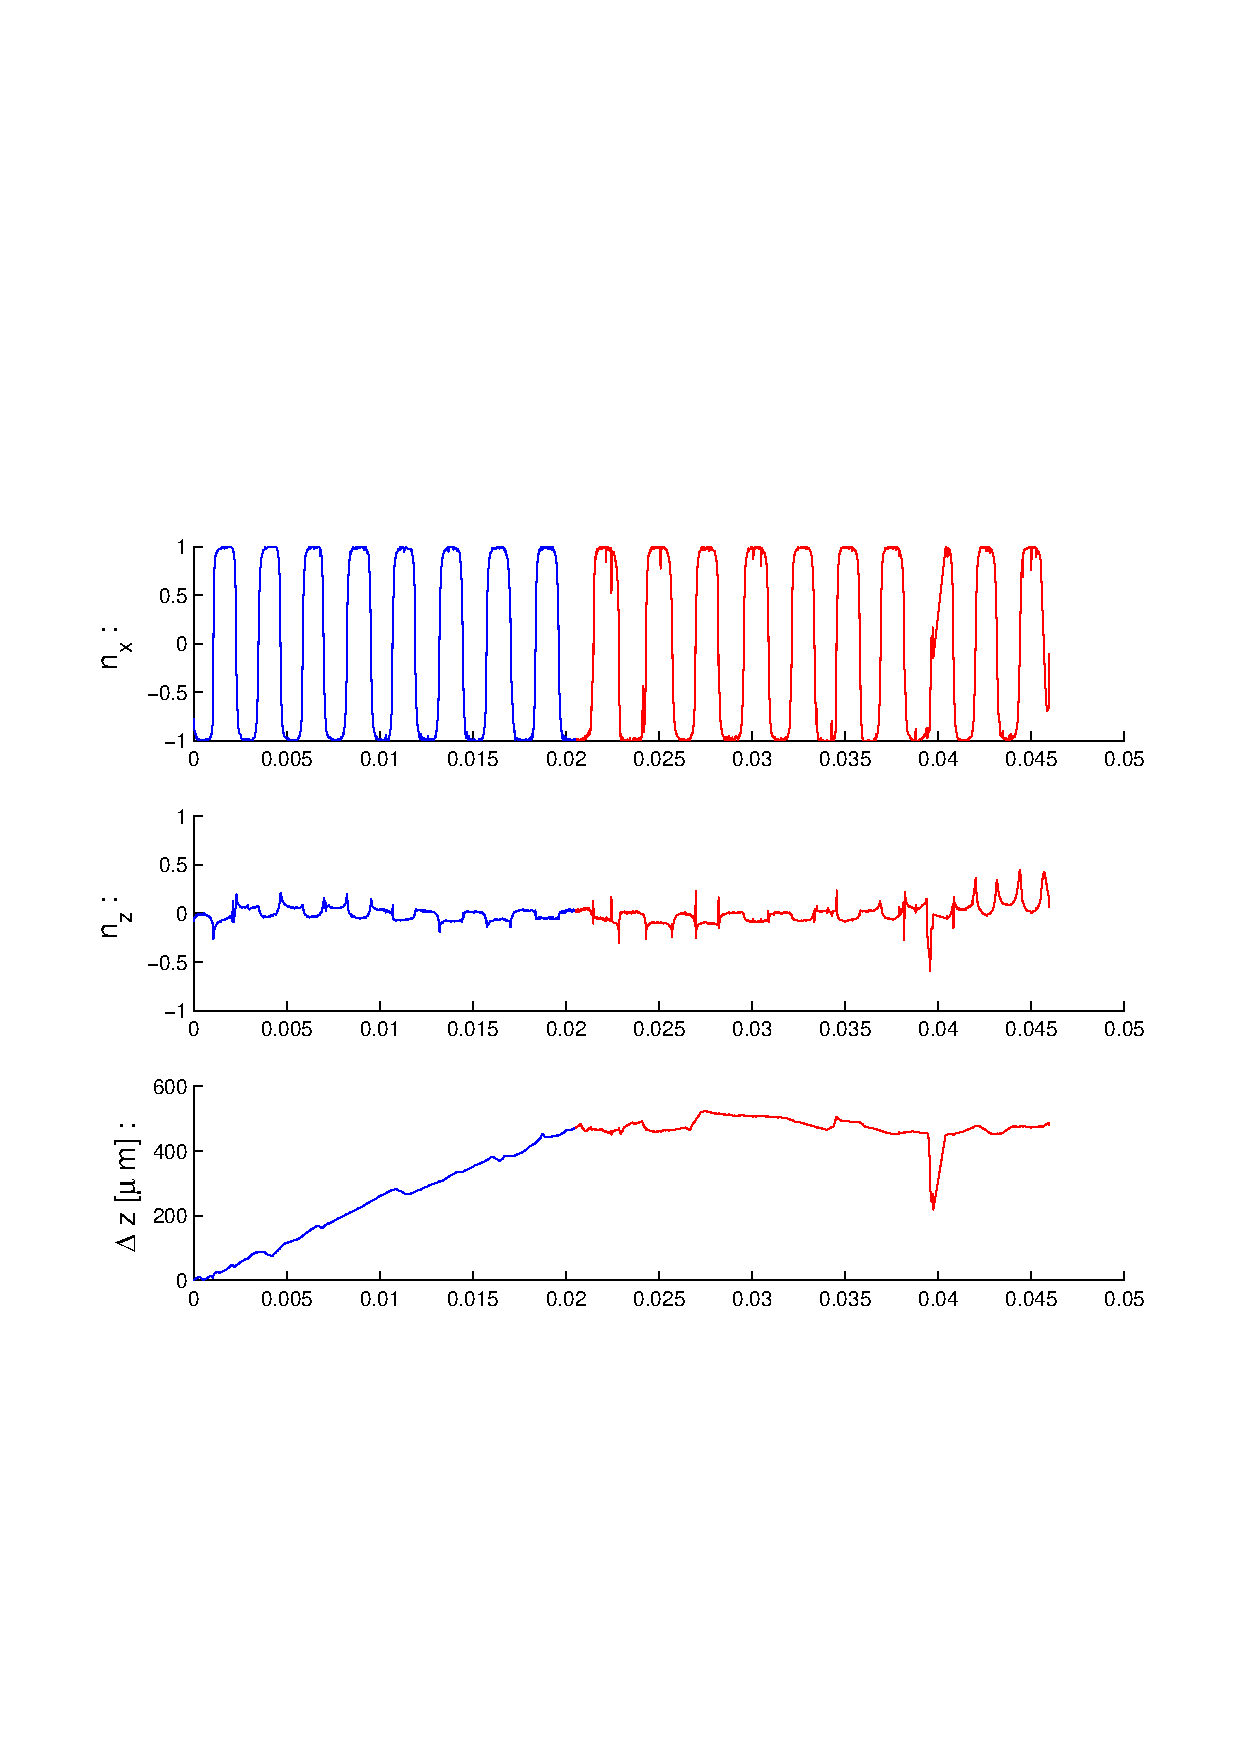
\includegraphics[width=0.8\textwidth]{Images/Particle 20/Particle20.pdf}

\end{figure}

\begin{figure}[ H]

\centering

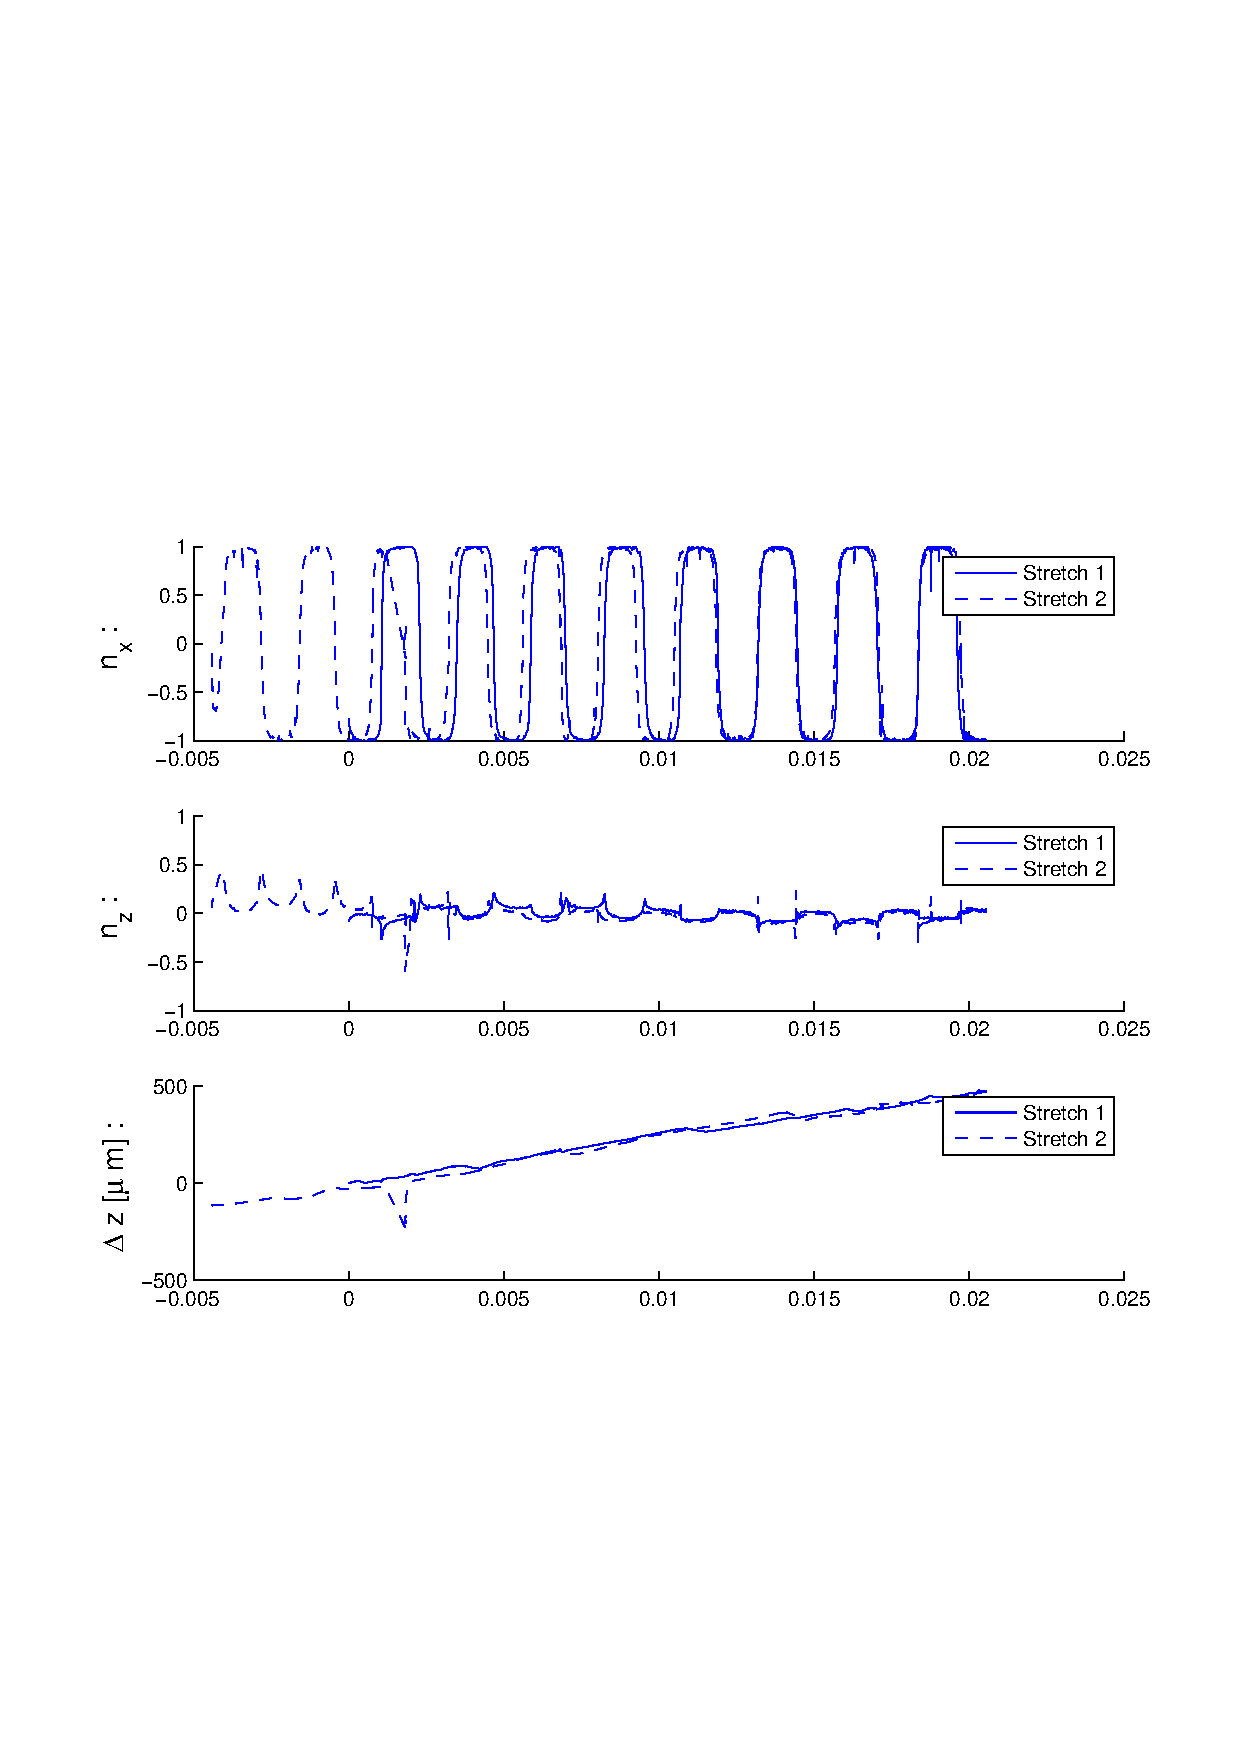
\includegraphics[width=0.8\textwidth]{Images/Particle 20/Stretch1.pdf}

\end{figure}



\subsection{Particle 24}

\begin{figure}[ H]

\caption{Particle 24: $ \lambda: 14.3715$Depth: 60 out of $200 \mu $ m}

\centering

\includegraphics[width=0.8\textwidth]{Images/Particle 24/Particle24.pdf}

\end{figure}

\begin{figure}[ H]

\centering

\includegraphics[width=0.8\textwidth]{Images/Particle 24/Stretch1.pdf}

\end{figure}

\begin{figure}[ H]

\centering

\includegraphics[width=0.8\textwidth]{Images/Particle 24/Stretch2.pdf}

\end{figure}

%
%\section{Other particles}
%\subsection{Particle 3}

\begin{figure}[H]

\includegraphics[width=0.8\textwidth]{Images/Particle 3/Particle3.pdf}

\caption{Particle 3:  $ \lambda: 19.5489$ Depth: 140 out of $200 \mu $ m}

\centering

\end{figure}

\begin{figure}[H]

\centering

\includegraphics[width=0.8\textwidth]{Images/Particle 3/Stretch1.pdf}

\end{figure}


\subsection{Particle 5}

\begin{figure}[H]

\includegraphics[width=0.8\textwidth]{Images/Particle 5/Particle5.pdf}

\caption{Particle 5:  $ \lambda: 15.2445$ Depth: 160 out of $200 \mu $ m}

\centering

\end{figure}

\begin{figure}[H]

\centering

\includegraphics[width=0.8\textwidth]{Images/Particle 5/Stretch1.pdf}

\end{figure}

\begin{figure}[H]

\centering

\includegraphics[width=0.8\textwidth]{Images/Particle 5/Stretch2.pdf}

\end{figure}


\subsection{Particle 6}

\begin{figure}[H]
\includegraphics[width=0.8\textwidth]{Images/Particle 6/Particle6.pdf}
\caption{Particle 6:  $ \lambda: 17.3351$ Depth: 150 out of $200 \mu $ m}
\centering

\end{figure}

\begin{figure}[H]

\centering

\includegraphics[width=0.8\textwidth]{Images/Particle 6/Stretch1.pdf}

\end{figure}

\begin{figure}[H]

\centering

\includegraphics[width=0.8\textwidth]{Images/Particle 6/Stretch2.pdf}

\end{figure}

\subsection{Particle 8}

\begin{figure}[H]

\includegraphics[width=0.8\textwidth]{Images/Particle 8/Particle8.pdf}

\caption{Particle 8:  $ \lambda: 36.1074$ Depth: 120 out of $200 \mu $ m}

\centering

\end{figure}

\subsection{Particle 9}

\begin{figure}[H]

\includegraphics[width=0.8\textwidth]{Images/Particle 9/Particle9.pdf}

\caption{Particle 9:  $ \lambda: 7.5902$ Depth: 160 out of $200 \mu $ m}

\centering

\end{figure}

\subsection{Particle 10}

\begin{figure}[H]

\includegraphics[width=0.8\textwidth]{Images/Particle 10/Particle10.pdf}

\caption{Particle 10:  $ \lambda: 8.6589$ Depth: 60 out of $200 \mu $ m}

\centering

\end{figure}

\begin{figure}[H]

\centering

\includegraphics[width=0.8\textwidth]{Images/Particle 10/Stretch1.pdf}

\end{figure}

\subsection{Particle 12}

\begin{figure}[H]

\includegraphics[width=0.8\textwidth]{Images/Particle 12/Particle12.pdf}

\caption{Particle 12:  $ \lambda: 8.1961$ Depth: 180 out of $200 \mu $ m}

\centering

\end{figure}

\begin{figure}[H]

\centering

\includegraphics[width=0.8\textwidth]{Images/Particle 12/Stretch1.pdf}

\end{figure}


\subsection{Particle 15}

\begin{figure}[H]

\includegraphics[width=0.8\textwidth]{Images/Particle 15/Particle15.pdf}

\caption{Particle 15:  $ \lambda: 7.7306$ Depth: 120 out of $200 \mu $ m}

\centering

\end{figure}

\begin{figure}[H]

\centering

\includegraphics[width=0.8\textwidth]{Images/Particle 15/Stretch1.pdf}

\end{figure}

\begin{figure}[H]

\centering

\includegraphics[width=0.8\textwidth]{Images/Particle 15/Stretch2.pdf}

\end{figure}


\subsection{Particle 17}

\begin{figure}[H]

\includegraphics[width=0.8\textwidth]{Images/Particle 17/Particle17.pdf}

\caption{Particle 17:  $ \lambda: 7.6562$ Depth: 180 out of $200 \mu $ m}

\centering

\end{figure}

\begin{figure}[H]

\centering

\includegraphics[width=0.8\textwidth]{Images/Particle 17/Stretch1.pdf}

\end{figure}

\begin{figure}[H]

\centering

\includegraphics[width=0.8\textwidth]{Images/Particle 17/Stretch2.pdf}

\end{figure}

\subsection{Particle 21}

\begin{figure}[H]

\includegraphics[width=0.8\textwidth]{Images/Particle 21/Particle21.pdf}

\caption{Particle 21:  $ \lambda: 9.6776$ Depth: 60 out of $200 \mu $ m}

\centering

\end{figure}

\begin{figure}[H]

\centering

\includegraphics[width=0.8\textwidth]{Images/Particle 21/Stretch1.pdf}

\end{figure}

\begin{figure}[H]

\centering

\includegraphics[width=0.8\textwidth]{Images/Particle 21/Stretch2.pdf}

\end{figure}

\bibliography{bibliography}
\bibliographystyle{plain}
\end{document}     
